\documentclass[a4paper]{book}
\usepackage{a4wide}
\usepackage{makeidx}
\usepackage{fancyhdr}
\usepackage{graphicx}
\usepackage{multicol}
\usepackage{float}
\usepackage{textcomp}
\usepackage{alltt}
\usepackage[utf8]{inputenc}
\usepackage{doxygen}
\makeindex
\setcounter{tocdepth}{3}
\renewcommand{\footrulewidth}{0.4pt}
\begin{document}
\begin{titlepage}
\vspace*{7cm}
\begin{center}
{\Large NeuroLab }\\
\vspace*{1cm}
{\large Generated by Doxygen 1.5.6}\\
\vspace*{0.5cm}
{\small Sun Dec 7 19:36:57 2008}\\
\end{center}
\end{titlepage}
\clearemptydoublepage
\pagenumbering{roman}
\tableofcontents
\clearemptydoublepage
\pagenumbering{arabic}
\chapter{Main Page}
\label{index}\section{Introduction}\label{main_Introduction}
NeuroLab is a class library which offers simulation of stochastic differential (integral) equations, as well as recording and display of data. Its main use is intended to be in the neuroscience field.\section{Principles}\label{main_General}
Stochastic Variables (\doxyref{StochasticVariable}{p.}{classStochasticVariable}), such as stochastic differential equations (\doxyref{DifferentialEquation}{p.}{classDifferentialEquation}), produce data. This data can be recorded (\doxyref{Matrix}{p.}{classMatrix}) by various estimators, which look for mean, variance and/or higher moments. Using a display (\doxyref{Display}{p.}{classDisplay}) the data can then be displayed, compared to analytical functions (\doxyref{Function}{p.}{classFunction}), and saved as data (gnuplot format), or postscript file, ready to be included in your paper.

Stochastic differential equations can be interpreted in the Ito or in the Stratonovich sense. The \doxyref{DifferentialEquation}{p.}{classDifferentialEquation} class lets you switch between these two versions, even at runtime.

Data can be recorded conditionally. This means the mean (or any other moment) of a process as function of the time distance to an observed event can be taken. This is done by a \doxyref{ConditionalEstimator}{p.}{classConditionalEstimator}, which records the time course of a stochastic variable (\doxyref{StochasticVariable}{p.}{classStochasticVariable}) before and after an observed event (Event).\section{Simulations}\label{main_Neural}
A leaky integrate-and-fire neuron is implemented (\doxyref{IfNeuron}{p.}{classIfNeuron}), which can be calibrated automatically to give a certain response rate (\doxyref{IfNeuron::calibrate()}{p.}{classIfNeuron_60f709212179b39774a1553463cd1b3a}). A neuron is also a SDE, so you may set up small neural networks, having a system of inter-dependent SDEs, where mutual dependencies are allowed as well. Since a neuron produces events (spikes), you can also do spike-triggered averaging.

A neuron may receive its stimulus via three different ways:

An independent stochastic process. These are objects of the classes \doxyref{Poisson}{p.}{classPoisson}, \doxyref{Wiener}{p.}{classWiener}, \doxyref{WienerCpp}{p.}{classWienerCpp}. They can be linked to a neuron with the \doxyref{IfNeuron::addStimulus()}{p.}{classIfNeuron_331ac02cfc9e7692bed845359db487ca} method. Each such object may drive one or many neurons.

A dependent stochastic process. A Noises object produces \doxyref{NoiseSource}{p.}{classNoiseSource} objects which resemble poisson and wiener processes, and which may be correlated. It is even possible to correlate a wiener and a poisson process.

Another neuron. In this case a synapse has to be built, which connects the neurons. Possible classes are \doxyref{Synapse}{p.}{classSynapse} (a simple synapse which transforms the spike events of the pre-synaptic neuron into Zeros and Ones [multiplied by a weight factor]), or \doxyref{SimpleSynapse}{p.}{classSimpleSynapse} (a more complex synapse, which is driven by a differential equation).\section{Quality}\label{main_Quality}
For a short quality check the equations \[dX_t = aX_tdt + bX_tdW_t\] (Ito) and \[dX_t = aX_tdt + bX_t\circ dW_t\] (Stratonovich) with $a=-8.0$ and $b=0.8$ are simulated using the \doxyref{DifferentialEquation}{p.}{classDifferentialEquation} class. This equation has an explicit solution, which was used to calculate the error (which is just the difference simulation - explicit solution in the following displays).

{\bf Step size = 0.1:} Above: Ito and Stratonovich equations plotted on top of their explicit solutions at a time step of 0.1ms.  Above: the error of the Ito and Stratonovich equations at a time step of 0.1ms.

{\bf  Step-size=0.01:}  Above: Ito and Stratonovich equations plotted on top of their explicit solutions at a time step of 0.01ms.  Above: the error of the Ito and Stratonovich equations at a time step of 0.01ms.

{\bf  Step-size=0.001:}  Above: Ito and Stratonovich equations plotted on top of their explicit solutions at a time step of 0.001ms.  Above: the error of the Ito and Stratonovich equations at a time step of 0.001ms. 
\chapter{Todo List}
\label{todo}
\label{todo__todo000001}
 \begin{description}
\item[Class \doxyref{Graph}{p.}{classGraph} ]Only two-dimensional graphs are implemented yet. Change this. \end{description}


\label{todo__todo000002}
 \begin{description}
\item[Class \doxyref{Matrix}{p.}{classMatrix} ]Implement \doxyref{Matrix}{p.}{classMatrix} multiplication and the (Matlab-known) functions cumsum, cummult and convolve for n-dimensional matrixes. \end{description}


\label{todo__todo000003}
 \begin{description}
\item[Class \doxyref{Noise}{p.}{classNoise} ]Finish implementing the noise class. \end{description}

\chapter{Class Index}
\section{Class Hierarchy}
This inheritance list is sorted roughly, but not completely, alphabetically:\begin{CompactList}
\item \contentsline{section}{DataCollector}{\pageref{classDataCollector}}{}
\item \contentsline{section}{Display}{\pageref{classDisplay}}{}
\item \contentsline{section}{DisplayAction}{\pageref{classDisplayAction}}{}
\item \contentsline{section}{IfNeuron}{\pageref{classIfNeuron}}{}
\item \contentsline{section}{Neuron}{\pageref{classNeuron}}{}
\item \contentsline{section}{NullStream}{\pageref{classNullStream}}{}
\item \contentsline{section}{Parametric}{\pageref{classParametric}}{}
\begin{CompactList}
\item \contentsline{section}{Estimator}{\pageref{classEstimator}}{}
\begin{CompactList}
\item \contentsline{section}{ConditionalEstimator}{\pageref{classConditionalEstimator}}{}
\item \contentsline{section}{ProcessEstimator}{\pageref{classProcessEstimator}}{}
\item \contentsline{section}{ScalarEstimator}{\pageref{classScalarEstimator}}{}
\begin{CompactList}
\item \contentsline{section}{IntervalEstimator}{\pageref{classIntervalEstimator}}{}
\end{CompactList}
\end{CompactList}
\item \contentsline{section}{StochasticProcess}{\pageref{classStochasticProcess}}{}
\begin{CompactList}
\item \contentsline{section}{Covariation}{\pageref{classCovariation}}{}
\item \contentsline{section}{NoiseSource}{\pageref{classNoiseSource}}{}
\item \contentsline{section}{StochasticFunction}{\pageref{classStochasticFunction}}{}
\begin{CompactList}
\item \contentsline{section}{Conductance}{\pageref{classConductance}}{}
\item \contentsline{section}{Product}{\pageref{classProduct}}{}
\begin{CompactList}
\item \contentsline{section}{Square}{\pageref{classSquare}}{}
\end{CompactList}
\item \contentsline{section}{Scalar}{\pageref{classScalar}}{}
\item \contentsline{section}{Synapse}{\pageref{classSynapse}}{}
\begin{CompactList}
\item \contentsline{section}{SimpleSynapse}{\pageref{classSimpleSynapse}}{}
\end{CompactList}
\item \contentsline{section}{ThetaMembrane}{\pageref{classThetaMembrane}}{}
\item \contentsline{section}{ThetaStimulus}{\pageref{classThetaStimulus}}{}
\end{CompactList}
\item \contentsline{section}{StochasticVariable}{\pageref{classStochasticVariable}}{}
\begin{CompactList}
\item \contentsline{section}{DifferentialEquation}{\pageref{classDifferentialEquation}}{}
\item \contentsline{section}{Noise}{\pageref{classNoise}}{}
\begin{CompactList}
\item \contentsline{section}{PoissonNoise}{\pageref{classPoissonNoise}}{}
\item \contentsline{section}{WienerNoise}{\pageref{classWienerNoise}}{}
\end{CompactList}
\item \contentsline{section}{StochasticEventGenerator}{\pageref{classStochasticEventGenerator}}{}
\begin{CompactList}
\item \contentsline{section}{Poisson}{\pageref{classPoisson}}{}
\end{CompactList}
\item \contentsline{section}{Wiener}{\pageref{classWiener}}{}
\begin{CompactList}
\item \contentsline{section}{WienerCpp}{\pageref{classWienerCpp}}{}
\end{CompactList}
\end{CompactList}
\end{CompactList}
\end{CompactList}
\item \contentsline{section}{Physical}{\pageref{classPhysical}}{}
\begin{CompactList}
\item \contentsline{section}{Function}{\pageref{classFunction}}{}
\item \contentsline{section}{Matrix}{\pageref{classMatrix}}{}
\begin{CompactList}
\item \contentsline{section}{Graph}{\pageref{classGraph}}{}
\end{CompactList}
\item \contentsline{section}{StochasticProcess}{\pageref{classStochasticProcess}}{}
\item \contentsline{section}{Time}{\pageref{classTime}}{}
\end{CompactList}
\item \contentsline{section}{Plot}{\pageref{classPlot}}{}
\item \contentsline{section}{Queue$<$ T $>$}{\pageref{classQueue}}{}
\item \contentsline{section}{RandN}{\pageref{classRandN}}{}
\begin{CompactList}
\item \contentsline{section}{NoiseSource}{\pageref{classNoiseSource}}{}
\item \contentsline{section}{Wiener}{\pageref{classWiener}}{}
\end{CompactList}
\item \contentsline{section}{ThetaNeuron}{\pageref{classThetaNeuron}}{}
\item \contentsline{section}{TimeDependent}{\pageref{classTimeDependent}}{}
\begin{CompactList}
\item \contentsline{section}{StochasticProcess}{\pageref{classStochasticProcess}}{}
\end{CompactList}
\item \contentsline{section}{Unit}{\pageref{classUnit}}{}
\end{CompactList}

\chapter{Class Index}
\section{Class List}
Here are the classes, structs, unions and interfaces with brief descriptions:\begin{CompactList}
\item\contentsline{section}{{\bf ConditionalEstimator} (Estimates conditional mean, var, etc. of a stochastic process )}{\pageref{classConditionalEstimator}}{}
\item\contentsline{section}{{\bf Conductance} (Returns a product of a difference of Xt )}{\pageref{classConductance}}{}
\item\contentsline{section}{{\bf Covariation} (\doxyref{Covariation}{p.}{classCovariation} process )}{\pageref{classCovariation}}{}
\item\contentsline{section}{{\bf DataCollector} (Class used to do user defined data collection in nested runs )}{\pageref{classDataCollector}}{}
\item\contentsline{section}{{\bf DifferentialEquation} (A stochastic differential equation )}{\pageref{classDifferentialEquation}}{}
\item\contentsline{section}{{\bf Display} (Class for displaying matrix data and analytical functions )}{\pageref{classDisplay}}{}
\item\contentsline{section}{{\bf DisplayAction} (An action object )}{\pageref{classDisplayAction}}{}
\item\contentsline{section}{{\bf Estimator} (Base class for estimation of various stochastic properties )}{\pageref{classEstimator}}{}
\item\contentsline{section}{{\bf Function} (Class for mathematical functions )}{\pageref{classFunction}}{}
\item\contentsline{section}{{\bf Graph} (The graph of a function )}{\pageref{classGraph}}{}
\item\contentsline{section}{{\bf IfNeuron} (Class implementing a simple integrate-and-fire neuron )}{\pageref{classIfNeuron}}{}
\item\contentsline{section}{{\bf IntervalEstimator} (Estimates interval distribution, mean, var, etc. of a time series )}{\pageref{classIntervalEstimator}}{}
\item\contentsline{section}{{\bf Matrix} (\doxyref{Matrix}{p.}{classMatrix} class )}{\pageref{classMatrix}}{}
\item\contentsline{section}{{\bf Neuron} (Class implementing a simple integrate-and-fire neuron )}{\pageref{classNeuron}}{}
\item\contentsline{section}{{\bf Noise} (A correlated noise source )}{\pageref{classNoise}}{}
\item\contentsline{section}{{\bf NoiseSource} (A set of mutually correlated noise sources (\doxyref{Wiener}{p.}{classWiener}, \doxyref{Poisson}{p.}{classPoisson} and Ornstein-Uhlenbeck processes) )}{\pageref{classNoiseSource}}{}
\item\contentsline{section}{{\bf NullStream} (Class used for piping output into nothingness )}{\pageref{classNullStream}}{}
\item\contentsline{section}{{\bf Parametric} (Class describing objects which can be parametrized )}{\pageref{classParametric}}{}
\item\contentsline{section}{{\bf Physical} (A physical value )}{\pageref{classPhysical}}{}
\item\contentsline{section}{{\bf Plot} (A plot descriptor used by the \doxyref{Display}{p.}{classDisplay} class )}{\pageref{classPlot}}{}
\item\contentsline{section}{{\bf Poisson} (Returns delta peaks with a static rate )}{\pageref{classPoisson}}{}
\item\contentsline{section}{{\bf PoissonNoise} (A poisson noise source )}{\pageref{classPoissonNoise}}{}
\item\contentsline{section}{{\bf ProcessEstimator} (Estimates mean, var, etc. of a stochastic process )}{\pageref{classProcessEstimator}}{}
\item\contentsline{section}{{\bf Product} (A product of the function input and a scalar )}{\pageref{classProduct}}{}
\item\contentsline{section}{{\bf Queue$<$ T $>$} (Small queue )}{\pageref{classQueue}}{}
\item\contentsline{section}{{\bf RandN} (An object which uses the randn function )}{\pageref{classRandN}}{}
\item\contentsline{section}{{\bf Scalar} (Returns a scalar )}{\pageref{classScalar}}{}
\item\contentsline{section}{{\bf ScalarEstimator} (Estimates mean, variance, etc. of a scalar stochastic variable )}{\pageref{classScalarEstimator}}{}
\item\contentsline{section}{{\bf SimpleSynapse} (A synapse )}{\pageref{classSimpleSynapse}}{}
\item\contentsline{section}{{\bf Square} (Returns the product of Xt$\ast$Xt and a scalar )}{\pageref{classSquare}}{}
\item\contentsline{section}{{\bf StochasticEventGenerator} (An object which generates events )}{\pageref{classStochasticEventGenerator}}{}
\item\contentsline{section}{{\bf StochasticFunction} (A parametrized stochastic variable )}{\pageref{classStochasticFunction}}{}
\item\contentsline{section}{{\bf StochasticProcess} (A stochastic variable )}{\pageref{classStochasticProcess}}{}
\item\contentsline{section}{{\bf StochasticVariable} (A simple stochastic variable )}{\pageref{classStochasticVariable}}{}
\item\contentsline{section}{{\bf Synapse} (A synapse )}{\pageref{classSynapse}}{}
\item\contentsline{section}{{\bf ThetaMembrane} (Theta neuron membranedecay term )}{\pageref{classThetaMembrane}}{}
\item\contentsline{section}{{\bf ThetaNeuron} (A Theta \doxyref{Neuron}{p.}{classNeuron} )}{\pageref{classThetaNeuron}}{}
\item\contentsline{section}{{\bf ThetaStimulus} (Theta neuron stimulus term )}{\pageref{classThetaStimulus}}{}
\item\contentsline{section}{{\bf Time} (The time )}{\pageref{classTime}}{}
\item\contentsline{section}{{\bf TimeDependent} (\doxyref{Time}{p.}{classTime} dependent objects )}{\pageref{classTimeDependent}}{}
\item\contentsline{section}{{\bf Unit} (A physical unit )}{\pageref{classUnit}}{}
\item\contentsline{section}{{\bf Wiener} (Properties for all \doxyref{Wiener}{p.}{classWiener} processes )}{\pageref{classWiener}}{}
\item\contentsline{section}{{\bf WienerCpp} (Condensed \doxyref{Poisson}{p.}{classPoisson} Process )}{\pageref{classWienerCpp}}{}
\item\contentsline{section}{{\bf WienerNoise} (A \doxyref{Wiener}{p.}{classWiener} process (white) noise source )}{\pageref{classWienerNoise}}{}
\end{CompactList}

\chapter{Class Documentation}
\section{ConditionalEstimator Class Reference}
\label{classConditionalEstimator}\index{ConditionalEstimator@{ConditionalEstimator}}
Inheritance diagram for ConditionalEstimator::\begin{figure}[H]
\begin{center}
\leavevmode
\includegraphics[height=3cm]{classConditionalEstimator}
\end{center}
\end{figure}


\subsection{Detailed Description}
estimates conditional mean, var, etc. of a stochastic process 

The conditional estimator records conditional probabilities. It links to a stochastic variable, and an event (both of which are given in the constructor). The variable and the state of the event are recorded each time prepareNextState() is called. If the event is true at a timestep, then the object will go on recording for a number of time steps, and then take all the properties. This enables you to take for instance the mean of a process at 20 time steps before to 10 time step after the occurance of a special event. In that case the 20 time steps would be given as 'pre', the 10 time steps as 'post' to the constructor. The main purpose of this class (at the time it was written) was the recording of spike-triggered averages in neurons. \subsection*{Public Member Functions}
\begin{CompactItemize}
\item 
{\bf ConditionalEstimator} (const Property \&property, {\bf StochasticProcess} $\ast$stochvar, {\bf StochasticEventGenerator} $\ast$condition, {\bf Time} $\ast$time, int pre, int post, int updateCorrection=0)
\begin{CompactList}\small\item\em Construct. \item\end{CompactList}\item 
{\bf ConditionalEstimator} (const Property \&property, {\bf StochasticProcess} $\ast$stochvar, {\bf StochasticProcess} $\ast$condition, {\bf Time} $\ast$time, int pre, int post, int updateCorrection=0)
\begin{CompactList}\small\item\em Construct. \item\end{CompactList}\item 
void {\bf setRejection} (int pre, int post)
\begin{CompactList}\small\item\em Add rejection interval. \item\end{CompactList}\item 
void {\bf removeRejection} ()
\begin{CompactList}\small\item\em Remove rejection. \item\end{CompactList}\item 
virtual void {\bf setParameter} (const Property \&p, double value)\label{classConditionalEstimator_f5f771f7cff9026af7109d76ccbd9159}

\begin{CompactList}\small\item\em set parameter value \item\end{CompactList}\item 
virtual void {\bf collect} ()\label{classConditionalEstimator_230301262ea04440adc4ce23ce682ace}

\begin{CompactList}\small\item\em receive next data point \item\end{CompactList}\item 
virtual {\bf Matrix} {\bf mResult} (const Property \&)\label{classConditionalEstimator_e9c71060bb7cd8504cfc3b509a82269c}

\begin{CompactList}\small\item\em get some property \item\end{CompactList}\item 
void {\bf init} ()\label{classConditionalEstimator_e3bb88958785255249e009c753387b53}

\begin{CompactList}\small\item\em initialize \item\end{CompactList}\item 
virtual {\bf $\sim$ConditionalEstimator} ()\label{classConditionalEstimator_db29e5b6cc1b148323ff3a95229d3a77}

\begin{CompactList}\small\item\em destruct \item\end{CompactList}\end{CompactItemize}


\subsection{Constructor \& Destructor Documentation}
\index{ConditionalEstimator@{ConditionalEstimator}!ConditionalEstimator@{ConditionalEstimator}}
\index{ConditionalEstimator@{ConditionalEstimator}!ConditionalEstimator@{ConditionalEstimator}}
\subsubsection[ConditionalEstimator]{\setlength{\rightskip}{0pt plus 5cm}ConditionalEstimator::ConditionalEstimator (const Property \& {\em property}, \/  {\bf StochasticProcess} $\ast$ {\em stochvar}, \/  {\bf StochasticEventGenerator} $\ast$ {\em condition}, \/  {\bf Time} $\ast$ {\em time}, \/  int {\em pre}, \/  int {\em post}, \/  int {\em updateCorrection} = {\tt 0})}\label{classConditionalEstimator_0e02d1b3e93f64249a3c93e4e57098ca}


Construct. 

This version constructs an object which records (and adds) samples of a stochastic process, depending on whether an event has occured: result = \{ stochvar(t), t in [pre,post] $|$ condition(0) \}. \begin{Desc}
\item[Parameters: ]\par
\begin{description}
\item[{\em 
property}]a collection of things to record \item[{\em 
stochvar}]the address of the stochastic variable to record \item[{\em 
condition}]the address of the event on which the recording is conditioned \item[{\em 
time}]the global time object \item[{\em 
pre}]number of time steps before the event \item[{\em 
post}]number of time steps after the event \item[{\em 
updateCorrection}]optional; defaults to 0. number of time steps to shift the result; this is to correct different update cascades \end{description}
\end{Desc}
\index{ConditionalEstimator@{ConditionalEstimator}!ConditionalEstimator@{ConditionalEstimator}}
\index{ConditionalEstimator@{ConditionalEstimator}!ConditionalEstimator@{ConditionalEstimator}}
\subsubsection[ConditionalEstimator]{\setlength{\rightskip}{0pt plus 5cm}ConditionalEstimator::ConditionalEstimator (const Property \& {\em property}, \/  {\bf StochasticProcess} $\ast$ {\em stochvar}, \/  {\bf StochasticProcess} $\ast$ {\em condition}, \/  {\bf Time} $\ast$ {\em time}, \/  int {\em pre}, \/  int {\em post}, \/  int {\em updateCorrection} = {\tt 0})}\label{classConditionalEstimator_a0efd957ebc4618af04d94a8b1c4e1c1}


Construct. 

This version constructs an object which records (and adds) samples of a stochastic process, multiplied with the value of another process: result = \{ stochvar(t)$\ast$condition(0), t in [pre,post] \}. \begin{Desc}
\item[Parameters: ]\par
\begin{description}
\item[{\em 
property}]a collection of things to record \item[{\em 
stochvar}]the address of the stochastic variable to record \item[{\em 
condition}]the address of the process on which the recording is conditioned \item[{\em 
time}]the global time object \item[{\em 
pre}]number of time steps before the event \item[{\em 
post}]number of time steps after the event \item[{\em 
updateCorrection}]optional; defaults to 0. number of time steps to shift the result; this is to correct different update cascades \end{description}
\end{Desc}


\subsection{Member Function Documentation}
\index{ConditionalEstimator@{ConditionalEstimator}!setRejection@{setRejection}}
\index{setRejection@{setRejection}!ConditionalEstimator@{ConditionalEstimator}}
\subsubsection[setRejection]{\setlength{\rightskip}{0pt plus 5cm}void ConditionalEstimator::setRejection (int {\em pre}, \/  int {\em post})}\label{classConditionalEstimator_293d7b5c39d64262cab391db5c92b09b}


Add rejection interval. 

Special. You will hardly ever need this. If a rejection interval is set, traces of the process where additional events fall into the interval -pre - post are rejected. (this changes the meausured process \[X_t\] to \[ Y_\tau = \{ X_{t+\tau} | c(t+\tau) \hat \not c(t+s), s \in [-pre,post]/0\}\] \begin{Desc}
\item[Parameters: ]\par
\begin{description}
\item[{\em 
pre}]start of rejection interval, counted from the event (t=0) \item[{\em 
post}]end of rejection interval, counted from the event (t=0) \end{description}
\end{Desc}
\index{ConditionalEstimator@{ConditionalEstimator}!removeRejection@{removeRejection}}
\index{removeRejection@{removeRejection}!ConditionalEstimator@{ConditionalEstimator}}
\subsubsection[removeRejection]{\setlength{\rightskip}{0pt plus 5cm}void ConditionalEstimator::removeRejection ()}\label{classConditionalEstimator_59b847386798c7910ab8ad2fc7a1bb9f}


Remove rejection. 

Sets the estimator to normal mode again. See \doxyref{setRejection()}{p.}{classConditionalEstimator_293d7b5c39d64262cab391db5c92b09b}. 
\section{Conductance Class Reference}
\label{classConductance}\index{Conductance@{Conductance}}
Inheritance diagram for Conductance::\begin{figure}[H]
\begin{center}
\leavevmode
\includegraphics[height=4cm]{classConductance}
\end{center}
\end{figure}


\subsection{Detailed Description}
returns a product of a difference of Xt 

A functional which implements a$\ast$(b - X\_\-t) \subsection*{Public Member Functions}
\begin{CompactItemize}
\item 
string {\bf getParameter} (const string \&)
\begin{CompactList}\small\item\em Get parameter. \item\end{CompactList}\item 
void {\bf setParameter} (const string \&name, const string \&value)
\begin{CompactList}\small\item\em Set parameter. \item\end{CompactList}\item 
virtual double {\bf calculateCurrentValue} ()\label{classConductance_d7eb693134d3a42da38527f6a2f0f941}

\begin{CompactList}\small\item\em Calculates the current value based on the current input. \item\end{CompactList}\item 
virtual double {\bf calculateNextValue} ()\label{classConductance_bbd40406c29e59f64c7d8f6e8c373199}

\begin{CompactList}\small\item\em Calculates the next value based on the current input. \item\end{CompactList}\end{CompactItemize}


\subsection{Member Function Documentation}
\index{Conductance@{Conductance}!getParameter@{getParameter}}
\index{getParameter@{getParameter}!Conductance@{Conductance}}
\subsubsection[getParameter]{\setlength{\rightskip}{0pt plus 5cm}string Conductance::getParameter (const string \& {\em name})\hspace{0.3cm}{\tt  [virtual]}}\label{classConductance_e7a8b09fa5096cbf0cb4fd2e08696a63}


Get parameter. 

In a derived class, override this to handle every parameter you implement. If a parameter is described using multiple strings separated by space, this indicates a parameter of a parameter. 

Reimplemented from {\bf Parametric} \doxyref{}{p.}{classParametric_3c39188e1750b8e5d442b9dfa079b1c8}.\index{Conductance@{Conductance}!setParameter@{setParameter}}
\index{setParameter@{setParameter}!Conductance@{Conductance}}
\subsubsection[setParameter]{\setlength{\rightskip}{0pt plus 5cm}void Conductance::setParameter (const string \& {\em name}, \/  const string \& {\em value})\hspace{0.3cm}{\tt  [virtual]}}\label{classConductance_f554e9cb35c3204747b1ce14a1024893}


Set parameter. 

Sets the value of a parameter using strings. If a parameter is described using multiple strings separated by space, this indicates a parameter of a parameter (not implemented yet). 

Reimplemented from {\bf Parametric} \doxyref{}{p.}{classParametric_bba36dc4545219658541ab55251e02e6}.
\section{Covariation Class Reference}
\label{classCovariation}\index{Covariation@{Covariation}}
Inheritance diagram for Covariation::\begin{figure}[H]
\begin{center}
\leavevmode
\includegraphics[height=3cm]{classCovariation}
\end{center}
\end{figure}


\subsection{Detailed Description}
\doxyref{Covariation}{p.}{classCovariation} process. 

The covariation process of two stochastic processes $X_t$ and $Y_t$ is defined as \[ \left[X,Y\right]_t = \int X_t dY_t + \int Y_t dX_t - X_tY_t. \] For deterministic processes this equals zero. The mean of this process is zero, if both processes $X_t$ and $Y_t$ are uncorrelated. The mean can be tested using a \doxyref{ProcessEstimator}{p.}{classProcessEstimator}. A covariation process can be used as integrator in differential equations. The \doxyref{Covariation}{p.}{classCovariation} class estimates the covariation process numerically, by using $\left[X,Y\right]_t = \int dX_t dY_t $. \subsection*{Public Member Functions}
\begin{CompactItemize}
\item 
{\bf Covariation} ({\bf StochasticProcess} $\ast$x, {\bf StochasticProcess} $\ast$y, string name=\char`\"{}\char`\"{}, const string \&type=\char`\"{}covariation\_\-process\char`\"{})
\begin{CompactList}\small\item\em Construct. \item\end{CompactList}\item 
{\bf $\sim$Covariation} ()\label{classCovariation_e054afdb4b91e25a30151b08c833601d}

\begin{CompactList}\small\item\em Destruct. \item\end{CompactList}\item 
void {\bf prepareNextState} ()
\begin{CompactList}\small\item\em Calculate next value. \item\end{CompactList}\end{CompactItemize}


\subsection{Constructor \& Destructor Documentation}
\index{Covariation@{Covariation}!Covariation@{Covariation}}
\index{Covariation@{Covariation}!Covariation@{Covariation}}
\subsubsection[Covariation]{\setlength{\rightskip}{0pt plus 5cm}Covariation::Covariation ({\bf StochasticProcess} $\ast$ {\em x}, \/  {\bf StochasticProcess} $\ast$ {\em y}, \/  string {\em name} = {\tt \char`\"{}\char`\"{}}, \/  const string \& {\em type} = {\tt \char`\"{}covariation\_\-process\char`\"{}})\hspace{0.3cm}{\tt  [inline]}}\label{classCovariation_7fdc96e02c656ffa70356995e0692d48}


Construct. 

This constructs a covariation prcoess of thwo stochastic processes. The resulting process is active by default, but can be set passive. 

\subsection{Member Function Documentation}
\index{Covariation@{Covariation}!prepareNextState@{prepareNextState}}
\index{prepareNextState@{prepareNextState}!Covariation@{Covariation}}
\subsubsection[prepareNextState]{\setlength{\rightskip}{0pt plus 5cm}void Covariation::prepareNextState ()\hspace{0.3cm}{\tt  [inline, virtual]}}\label{classCovariation_44472092d0752fb1c485012b46f4d47e}


Calculate next value. 

If the process is active, this is called automatically. If it is passive, call \doxyref{proceedToNextState()}{p.}{classStochasticProcess_c79b6846db19a8de5025a2e36b6f6901} first, and then \doxyref{prepareNextState()}{p.}{classCovariation_44472092d0752fb1c485012b46f4d47e}, to complete a full step.. 

Reimplemented from {\bf StochasticProcess} \doxyref{}{p.}{classStochasticProcess_b4c11ea89fa2d41a9f61df1ebdf04f78}.
\section{DataCollector Class Reference}
\label{classDataCollector}\index{DataCollector@{DataCollector}}


\subsection{Detailed Description}
Class used to do user defined data collection in nested runs. \subsection*{Public Member Functions}
\begin{CompactItemize}
\item 
virtual void {\bf beforeRun} (const vector$<$ unsigned long long int $>$ \&step)=0\label{classDataCollector_0f9ab7094ea0a6b0bfbec4cb8522b4ed}

\begin{CompactList}\small\item\em Will be executed before each run. \item\end{CompactList}\item 
virtual void {\bf afterRun} (const vector$<$ unsigned long long int $>$ \&step)=0\label{classDataCollector_fa23a704c60999eeb9344d87f7b2edf0}

\begin{CompactList}\small\item\em Will be executed after each run. \item\end{CompactList}\end{CompactItemize}

\section{DifferentialEquation Class Reference}
\label{classDifferentialEquation}\index{DifferentialEquation@{DifferentialEquation}}
Inheritance diagram for DifferentialEquation::\begin{figure}[H]
\begin{center}
\leavevmode
\includegraphics[height=4cm]{classDifferentialEquation}
\end{center}
\end{figure}


\subsection{Detailed Description}
A stochastic differential equation. 

Class implementing stochastic differential equations (SDEs). Ito- and Stratonovich integrals can be chosen, integrators and integrands can be added at runtime.

This class implements stochastic differential equations (SDEs) of the form \[ dX = \sum_i f_i(X) dY_i \] (using It$\backslash$$^\wedge$o integrals), or \[ dX = \sum_i f_i(X) \circ dY_i \] (using Stratonovich integrals). The sum goes over multiple different functions $f_i$. These should be intepreted as integral equations of the form \[ X - X_0 = \sum_i \intop f_i(X) dY_i \] (Ito), or \[ X - X_0 = \sum_i \intop f_i(X) \circ dY_i \] (Stratonovich). It$\backslash$$^\wedge$o mode can be set by calling \doxyref{setIto()}{p.}{classDifferentialEquation_66d03f1596bf45447470584d926b315e}, Stratonovich mode can be set by calling \doxyref{setStrat()}{p.}{classDifferentialEquation_9780bdc8678ef3ee087a677009355248}. Which mode is used can be tested by querying \doxyref{bIsIto()}{p.}{classDifferentialEquation_a7a176d030187ecf334b9bf3299fd140} (true if Ito mode) or \doxyref{bIsStrat()}{p.}{classDifferentialEquation_c0a680c1486cac02b048cbdf475b5d61} (true if Stratonovich integrals are used). At the moment there is only the 0.5-strong-order Euler scheme implemented, but Milstein and Taylor of higher order are planned for the future. See the main page for display of the error made when integrating. Here is a short example of the difference of Ito and Stratonovich integration (the equation is $dX_t = aX_tdt + bX_tdW_t$ or $dX_t = aX_tdt + bX_t\circ dW_t$ with $a=-8.0$ and $b=0.8$.):

The integrands $f_i(X_t)$ are objects of the type Integrand, and the integrators $dY_i$ are objects of the type Integrator. They are stored in arrays of function objects, and their Integrand::operator()(double) or Integrator::operator()() are called each time \doxyref{proceedToNextState()}{p.}{classStochasticProcess_c79b6846db19a8de5025a2e36b6f6901} is called. Use dGetValue() (from StochVar) or operator(double) to get the current value of the integral. The function \doxyref{proceedToNextState()}{p.}{classStochasticProcess_c79b6846db19a8de5025a2e36b6f6901} must be used to calculate the values of the next time step, the function \doxyref{prepareNextState()}{p.}{classDifferentialEquation_439f935ee6aac295651739607795b3f2} must be used to update the object. New integrators and integrands may be added easily by calling nAddIntegrator() or nAddIntegrand().

\doxyref{DifferentialEquation}{p.}{classDifferentialEquation} itself is of type Integrator and of type Integrand, so complex cascades of differential equations may be implemented. If you have a complex network of interdependent SDEs, you must first call the \doxyref{proceedToNextState()}{p.}{classStochasticProcess_c79b6846db19a8de5025a2e36b6f6901} function of all objects, then the \doxyref{prepareNextState()}{p.}{classDifferentialEquation_439f935ee6aac295651739607795b3f2} function of all objects. Otherwise circular dependencies will not get updated correctly. \subsection*{Ito/Stratonovich mode}
\begin{CompactItemize}
\item 
void(DifferentialEquation::$\ast$ {\bf eqnMethodPtr} )()\label{classDifferentialEquation_0be894b3b8606b82be65a2e8ca05f59b}

\begin{CompactList}\small\item\em member pointer to one of the privat fcns. \item\end{CompactList}\item 
bool {\bf bIsIto} ()\label{classDifferentialEquation_a7a176d030187ecf334b9bf3299fd140}

\begin{CompactList}\small\item\em ito integrating mode? \item\end{CompactList}\item 
bool {\bf bIsStrat} ()\label{classDifferentialEquation_c0a680c1486cac02b048cbdf475b5d61}

\begin{CompactList}\small\item\em stratonovich integrating mode? \item\end{CompactList}\item 
void {\bf setIto} ()\label{classDifferentialEquation_66d03f1596bf45447470584d926b315e}

\begin{CompactList}\small\item\em set integrating mode to ito \item\end{CompactList}\item 
void {\bf setStrat} ()\label{classDifferentialEquation_9780bdc8678ef3ee087a677009355248}

\begin{CompactList}\small\item\em set integrating mode to stratonovich \item\end{CompactList}\end{CompactItemize}
\subsection*{Public Member Functions}
\begin{CompactItemize}
\item 
{\bf DifferentialEquation} (double x0, double dx0, const string \&name=\char`\"{}\char`\"{}, const string \&type=\char`\"{}differential\_\-equation\char`\"{})
\begin{CompactList}\small\item\em starting value \item\end{CompactList}\item 
{\bf DifferentialEquation} ({\bf Time} $\ast$time, double x0, double dx0, const string \&name=\char`\"{}\char`\"{}, const string \&type=\char`\"{}differential\_\-equation\char`\"{})
\begin{CompactList}\small\item\em Constructor. \item\end{CompactList}\item 
{\bf DifferentialEquation} (const string \&name=\char`\"{}\char`\"{}, const string \&type=\char`\"{}differential\_\-equation\char`\"{})
\begin{CompactList}\small\item\em Construct. \item\end{CompactList}\item 
virtual {\bf $\sim$DifferentialEquation} ()\label{classDifferentialEquation_10ec69c81f274c4efa28272bb2d90fd0}

\begin{CompactList}\small\item\em Destructor. \item\end{CompactList}\item 
virtual void {\bf prepareNextState} ()
\begin{CompactList}\small\item\em Calculate value for next time step. \item\end{CompactList}\item 
virtual void {\bf init} (double x0)\label{classDifferentialEquation_b57ce9c7abd5afbe1ffc3e56d8f8d1b9}

\begin{CompactList}\small\item\em Sets value to a starting value. \item\end{CompactList}\item 
virtual void {\bf init} ()\label{classDifferentialEquation_69375f9237ad9af5b2c25715b98e3337}

\begin{CompactList}\small\item\em Sets value to starting value. \item\end{CompactList}\item 
double {\bf getStartingValue} ()\label{classDifferentialEquation_576049bb5a2b986ada3771fe10c8c108}

\begin{CompactList}\small\item\em Get the starting value. \item\end{CompactList}\item 
int {\bf addTerm} ({\bf StochasticFunction} $\ast$integrand, {\bf StochasticVariable} $\ast$integrator)\label{classDifferentialEquation_1bef85199f80682b84a9f9645a65d0bf}

\begin{CompactList}\small\item\em Add term. \item\end{CompactList}\item 
void {\bf rmTerm} (int n)\label{classDifferentialEquation_00c79559c2436f9b09efe619fc578ff7}

\begin{CompactList}\small\item\em Remove term. \item\end{CompactList}\item 
void {\bf setTerm} (int n, {\bf StochasticFunction} $\ast$integrand, {\bf StochasticVariable} $\ast$integrator)\label{classDifferentialEquation_bacb88e73ac01d5b1046a46d758e0292}

\begin{CompactList}\small\item\em Set term. \item\end{CompactList}\item 
{\bf StochasticFunction} $\ast$ {\bf getIntegrand} (int)\label{classDifferentialEquation_d9770baa4710ee0135a1b0542726b935}

\begin{CompactList}\small\item\em get integrand \item\end{CompactList}\item 
{\bf StochasticVariable} $\ast$ {\bf getIntegrator} (int)\label{classDifferentialEquation_828d89a67bf32e8e4406586e826fa9b5}

\begin{CompactList}\small\item\em get integrator \item\end{CompactList}\item 
virtual string {\bf getParameter} (const string \&name)
\begin{CompactList}\small\item\em Get parameter. \item\end{CompactList}\end{CompactItemize}


\subsection{Constructor \& Destructor Documentation}
\index{DifferentialEquation@{DifferentialEquation}!DifferentialEquation@{DifferentialEquation}}
\index{DifferentialEquation@{DifferentialEquation}!DifferentialEquation@{DifferentialEquation}}
\subsubsection[DifferentialEquation]{\setlength{\rightskip}{0pt plus 5cm}DifferentialEquation::DifferentialEquation (double {\em x0}, \/  double {\em dx0}, \/  const string \& {\em name} = {\tt \char`\"{}\char`\"{}}, \/  const string \& {\em type} = {\tt \char`\"{}differential\_\-equation\char`\"{}})}\label{classDifferentialEquation_f690efd96c3aeee8d957e93d8be3129c}


starting value 

Constructor. \begin{Desc}
\item[Parameters:]
\begin{description}
\item[{\em x0}]Starting value \item[{\em dx0}]Starting increment \end{description}
\end{Desc}
\index{DifferentialEquation@{DifferentialEquation}!DifferentialEquation@{DifferentialEquation}}
\index{DifferentialEquation@{DifferentialEquation}!DifferentialEquation@{DifferentialEquation}}
\subsubsection[DifferentialEquation]{\setlength{\rightskip}{0pt plus 5cm}DifferentialEquation::DifferentialEquation ({\bf Time} $\ast$ {\em time}, \/  double {\em x0}, \/  double {\em dx0}, \/  const string \& {\em name} = {\tt \char`\"{}\char`\"{}}, \/  const string \& {\em type} = {\tt \char`\"{}differential\_\-equation\char`\"{}})}\label{classDifferentialEquation_d812fc6333f3899719220652b94514b6}


Constructor. 

\begin{Desc}
\item[Parameters:]
\begin{description}
\item[{\em x0}]Starting value \item[{\em dx0}]Starting increment \end{description}
\end{Desc}
\index{DifferentialEquation@{DifferentialEquation}!DifferentialEquation@{DifferentialEquation}}
\index{DifferentialEquation@{DifferentialEquation}!DifferentialEquation@{DifferentialEquation}}
\subsubsection[DifferentialEquation]{\setlength{\rightskip}{0pt plus 5cm}DifferentialEquation::DifferentialEquation (const string \& {\em name} = {\tt \char`\"{}\char`\"{}}, \/  const string \& {\em type} = {\tt \char`\"{}differential\_\-equation\char`\"{}})\hspace{0.3cm}{\tt  [inline]}}\label{classDifferentialEquation_ba36a02def7ec519975e057b70298480}


Construct. 

The same as using \doxyref{DifferentialEquation}{p.}{classDifferentialEquation}(0.0, 0.0). 

\subsection{Member Function Documentation}
\index{DifferentialEquation@{DifferentialEquation}!prepareNextState@{prepareNextState}}
\index{prepareNextState@{prepareNextState}!DifferentialEquation@{DifferentialEquation}}
\subsubsection[prepareNextState]{\setlength{\rightskip}{0pt plus 5cm}virtual void DifferentialEquation::prepareNextState ()\hspace{0.3cm}{\tt  [virtual]}}\label{classDifferentialEquation_439f935ee6aac295651739607795b3f2}


Calculate value for next time step. 

This just calculates the next value. Nothing is changed before \doxyref{proceedToNextState()}{p.}{classStochasticProcess_c79b6846db19a8de5025a2e36b6f6901} is called. 

Reimplemented from {\bf StochasticProcess} \doxyref{}{p.}{classStochasticProcess_b4c11ea89fa2d41a9f61df1ebdf04f78}.\index{DifferentialEquation@{DifferentialEquation}!getParameter@{getParameter}}
\index{getParameter@{getParameter}!DifferentialEquation@{DifferentialEquation}}
\subsubsection[getParameter]{\setlength{\rightskip}{0pt plus 5cm}virtual string DifferentialEquation::getParameter (const string \& {\em name})\hspace{0.3cm}{\tt  [virtual]}}\label{classDifferentialEquation_8edfa603b974d803268a604dff8ff964}


Get parameter. 

In a derived class, override this to handle every parameter you implement. If a parameter is described using multiple strings separated by space, this indicates a parameter of a parameter. \begin{Desc}
\item[Parameters: ]\par
\begin{description}
\item[{\em 
name}]name of parameter \end{description}
\end{Desc}


Reimplemented from {\bf Parametric} \doxyref{}{p.}{classParametric_3c39188e1750b8e5d442b9dfa079b1c8}.
\section{Display Class Reference}
\label{classDisplay}\index{Display@{Display}}


\subsection{Detailed Description}
Class for displaying matrix data and analytical functions. 

\doxyref{Display}{p.}{classDisplay} data given as Matrixes or as strings describing functions in various forms. Currently there is only an interface to gnuplot implemented, others shall follow (qwt, grace, qplotter). \subsection*{Public Member Functions}
\begin{CompactItemize}
\item 
{\bf Display} (const char $\ast$filebase)
\begin{CompactList}\small\item\em constructor \item\end{CompactList}\item 
{\bf $\sim$Display} ()\label{classDisplay_c2607a6bb236c55547a4223d40d85d1f}

\begin{CompactList}\small\item\em destructor \item\end{CompactList}\item 
void {\bf show} ()
\begin{CompactList}\small\item\em Show data as plot. \item\end{CompactList}\item 
void {\bf save} ()
\begin{CompactList}\small\item\em Save data to postscript file. \item\end{CompactList}\item 
void {\bf setMode} (const int \&mode)
\begin{CompactList}\small\item\em Set mode. \item\end{CompactList}\item 
void {\bf setLineStyle} (const int \&style)
\begin{CompactList}\small\item\em Set line style. \item\end{CompactList}\item 
void {\bf addMode} (const int \&mode)\label{classDisplay_49fe2c2526dbdd0d465776f1bdaf8fdc}

\begin{CompactList}\small\item\em Add mode. \item\end{CompactList}\item 
void {\bf rmMode} (const int \&mode)\label{classDisplay_0b89ea9df85b7bd1dd36492bdd3a6cb0}

\begin{CompactList}\small\item\em Remove mode. \item\end{CompactList}\item 
void {\bf setTitle} (string title)
\begin{CompactList}\small\item\em Set title. \item\end{CompactList}\item 
void {\bf addUserSetting} (string s)
\begin{CompactList}\small\item\em Add user setting. \item\end{CompactList}\item 
void {\bf clearUserSettings} ()\label{classDisplay_35da8930e26c0cc6c80b84cb3e913d13}

\begin{CompactList}\small\item\em Clears all user settings. \item\end{CompactList}\item 
{\bf Display} \& {\bf operator$<$$<$} ({\bf Matrix} m)
\begin{CompactList}\small\item\em Insert matrix data. \item\end{CompactList}\item 
{\bf Display} \& {\bf operator$<$$<$} ({\bf Function} \&f)
\begin{CompactList}\small\item\em Insert function. \item\end{CompactList}\item 
{\bf Display} \& {\bf operator$<$$<$} (const class {\bf DisplayAction} \&a)
\begin{CompactList}\small\item\em Execute modification or action. \item\end{CompactList}\end{CompactItemize}


\subsection{Constructor \& Destructor Documentation}
\index{Display@{Display}!Display@{Display}}
\index{Display@{Display}!Display@{Display}}
\subsubsection[Display]{\setlength{\rightskip}{0pt plus 5cm}Display::Display (const char $\ast$ {\em filebase})}\label{classDisplay_5fee2391c213e91cca7920dd6267cf53}


constructor 

\begin{Desc}
\item[Parameters:]
\begin{description}
\item[{\em filebase}]A string which will be used to construct the filenames, which will be called [filebase]000.dat, [filebase]001.dat, ... for the data files, and [filebase].gnuplot for the gnuplot instruction file. Constructs a display. The input argument file is used to create files in which to store data for gnuplot / grace. The will be named filebase.xxx.data, where xxx is a decimal integer running from 000 to 999 (depending on the number of files). After destruction these will not be deleted. \end{description}
\end{Desc}


\subsection{Member Function Documentation}
\index{Display@{Display}!show@{show}}
\index{show@{show}!Display@{Display}}
\subsubsection[show]{\setlength{\rightskip}{0pt plus 5cm}void Display::show ()}\label{classDisplay_8f37df54881eebc4eba88190f77b854b}


Show data as plot. 

This displays the data. It opens a terminal with a gnuplot-session, with the data already plotted. The user may close the terminal and/or gnuplot window, or use the terminal to add more plots to the gnuplot window. \index{Display@{Display}!save@{save}}
\index{save@{save}!Display@{Display}}
\subsubsection[save]{\setlength{\rightskip}{0pt plus 5cm}void Display::save ()}\label{classDisplay_44a6a950b4495917cdb4ba80f085b084}


Save data to postscript file. 

This saves the data. The raw data is saved anyway, this function saves the postscript file which you want to include in your paper. \index{Display@{Display}!setMode@{setMode}}
\index{setMode@{setMode}!Display@{Display}}
\subsubsection[setMode]{\setlength{\rightskip}{0pt plus 5cm}void Display::setMode (const int \& {\em mode})}\label{classDisplay_1ddc351f26a035765f4a52ed67eae9fe}


Set mode. 

Sets the display mode. A mode is an $|$-list of values. This must be done $\ast$before$\ast$ the first data is inserted using the $<$$<$ operator. Current values are DSP\_\-3D, DSP\_\-2D, DSP\_\-INCLUDE\_\-START, DSP\_\-INCLUDE\_\-END \index{Display@{Display}!setLineStyle@{setLineStyle}}
\index{setLineStyle@{setLineStyle}!Display@{Display}}
\subsubsection[setLineStyle]{\setlength{\rightskip}{0pt plus 5cm}void Display::setLineStyle (const int \& {\em style})}\label{classDisplay_9550c9ce06b93e8b57c4d99c8bca2a3e}


Set line style. 

Sets the line style of the last plot. Style is an integer $>$= 0. In gnuplot, if many plots are executed, each plot gets a different colour (if in colour mode), or line style like dottet, dashed, etc. (if in monochrome mode). Using the setLineStyle function you can override this for the plot added last, and can specify a certain value (if you want multiple lines in the same color, for instance). If style==0, gnuplot defaults are used. \index{Display@{Display}!setTitle@{setTitle}}
\index{setTitle@{setTitle}!Display@{Display}}
\subsubsection[setTitle]{\setlength{\rightskip}{0pt plus 5cm}void Display::setTitle (string {\em title})}\label{classDisplay_dacf8d34743086bd18fae31e2fddd0b6}


Set title. 

\begin{Desc}
\item[Parameters:]
\begin{description}
\item[{\em title}]The title. This is the title of the plot, written abouve the actual plot in gnuplot. \end{description}
\end{Desc}
\index{Display@{Display}!addUserSetting@{addUserSetting}}
\index{addUserSetting@{addUserSetting}!Display@{Display}}
\subsubsection[addUserSetting]{\setlength{\rightskip}{0pt plus 5cm}void Display::addUserSetting (string {\em s})}\label{classDisplay_c863fc7294fcf78ddd9b62eeb98a08c4}


Add user setting. 

This adds a user setting. The given string will be handed over to gnuplot before the first plot data is made. Example: dsp.addUserSetting(\char`\"{}set yrange [-20:20]\char`\"{}); will set the y range to the given interval. It is also possible to add a comment here, which will then appear in the gnuplot file (handy if you want to understand what's in that file you've produced three months ago); Example: dsp.addUserSetting(\char`\"{}\# this contains the simulated output of an integrate-and-fire neuron with firing rate of 10Hz\char`\"{});. \index{Display@{Display}!operator$<$$<$@{operator$<$$<$}}
\index{operator$<$$<$@{operator$<$$<$}!Display@{Display}}
\subsubsection[operator$<$$<$]{\setlength{\rightskip}{0pt plus 5cm}{\bf Display}\& Display::operator$<$$<$ ({\bf Matrix} {\em m})}\label{classDisplay_a865ea3e4f642e62c2f5fedc161fc62b}


Insert matrix data. 

This appends some data to the current display. Use \doxyref{show()}{p.}{classDisplay_8f37df54881eebc4eba88190f77b854b} to display all data. \index{Display@{Display}!operator$<$$<$@{operator$<$$<$}}
\index{operator$<$$<$@{operator$<$$<$}!Display@{Display}}
\subsubsection[operator$<$$<$]{\setlength{\rightskip}{0pt plus 5cm}{\bf Display}\& Display::operator$<$$<$ ({\bf Function} \& {\em f})}\label{classDisplay_521d04ca7b322c2e210a5c73b7696398}


Insert function. 

This appends a function to plot to the current display. The stream must describe a string string which evaluates in gnuplot. Use \doxyref{show()}{p.}{classDisplay_8f37df54881eebc4eba88190f77b854b} to display all data and functions which have been inserted. \index{Display@{Display}!operator$<$$<$@{operator$<$$<$}}
\index{operator$<$$<$@{operator$<$$<$}!Display@{Display}}
\subsubsection[operator$<$$<$]{\setlength{\rightskip}{0pt plus 5cm}{\bf Display}\& Display::operator$<$$<$ (const class {\bf DisplayAction} \& {\em a})}\label{classDisplay_9c8c25a0862e708d75cc1da19198d709}


Execute modification or action. 

This executes a modification (like dsp $<$$<$ set3d;) or an action (like dsp $<$$<$ show;). See the documentation for \doxyref{DisplayAction}{p.}{classDisplayAction} objects. 
\section{DisplayAction Class Reference}
\label{classDisplayAction}\index{DisplayAction@{DisplayAction}}


\subsection{Detailed Description}
An action object. 

This object can be appended to modify a \doxyref{Display}{p.}{classDisplay} object, or to execute an action. \subsection*{Public Member Functions}
\begin{CompactItemize}
\item 
void {\bf execute} ({\bf Display} $\ast$d) const \label{classDisplayAction_4d1f5efc9682f759b67b5a72670c3116}

\begin{CompactList}\small\item\em Execute one of my members. \item\end{CompactList}\end{CompactItemize}

\section{Estimator Class Reference}
\label{classEstimator}\index{Estimator@{Estimator}}
Inheritance diagram for Estimator::\begin{figure}[H]
\begin{center}
\leavevmode
\includegraphics[height=4cm]{classEstimator}
\end{center}
\end{figure}


\subsection{Detailed Description}
Base class for estimation of various stochastic properties. 

Estimates various properties of stochastic variables (like mean, variance, density). An estimator receives a source of the type \doxyref{StochasticProcess}{p.}{classStochasticProcess}, of which it receives the data during every step (every time proceedToNextState() is called). \subsection*{Public Member Functions}
\begin{CompactItemize}
\item 
{\bf Estimator} ({\bf StochasticProcess} $\ast$src, {\bf Time} $\ast$time, const string \&name=\char`\"{}\char`\"{}, const string \&type=\char`\"{}estimator\char`\"{})
\begin{CompactList}\small\item\em Construct. \item\end{CompactList}\item 
virtual void {\bf init} ()=0\label{classEstimator_02466dbd2cd9dd016c9d34e6ddfe0500}

\begin{CompactList}\small\item\em Reset all estimation dependent values. \item\end{CompactList}\item 
virtual {\bf $\sim$Estimator} ()
\begin{CompactList}\small\item\em Destroy. \item\end{CompactList}\item 
virtual void {\bf collect} ()=0\label{classEstimator_412c13e686e39bbabdc6d1a2405f35dd}

\begin{CompactList}\small\item\em Eat the next data point. \item\end{CompactList}\item 
virtual {\bf Matrix} {\bf mResult} (const Property \&)=0\label{classEstimator_ff1c3031eea5b7c93c2d3efd23550eda}

\begin{CompactList}\small\item\em Return an estimation. \item\end{CompactList}\end{CompactItemize}
\subsection*{Protected Attributes}
\begin{CompactItemize}
\item 
Property {\bf nEstimate}\label{classEstimator_295e284fbc86aaca93e9c0a05a7ff80d}

\begin{CompactList}\small\item\em what to record \item\end{CompactList}\item 
{\bf StochasticProcess} $\ast$ {\bf pSource}\label{classEstimator_536a0926982bbe5d01fdb0d54f258523}

\begin{CompactList}\small\item\em the source of data \item\end{CompactList}\item 
uint {\bf nSamples}\label{classEstimator_1da705bea2733f5ade41b487e2a449dd}

\begin{CompactList}\small\item\em number of samples recorded \item\end{CompactList}\item 
{\bf Time} $\ast$ {\bf estimatorTime}\label{classEstimator_53aed902d3be7985bcc13ce6d10f1e8a}

\begin{CompactList}\small\item\em \doxyref{Time}{p.}{classTime} process for registering and running. \item\end{CompactList}\end{CompactItemize}


\subsection{Constructor \& Destructor Documentation}
\index{Estimator@{Estimator}!Estimator@{Estimator}}
\index{Estimator@{Estimator}!Estimator@{Estimator}}
\subsubsection[Estimator]{\setlength{\rightskip}{0pt plus 5cm}Estimator::Estimator ({\bf StochasticProcess} $\ast$ {\em src}, \/  {\bf Time} $\ast$ {\em time}, \/  const string \& {\em name} = {\tt \char`\"{}\char`\"{}}, \/  const string \& {\em type} = {\tt \char`\"{}estimator\char`\"{}})}\label{classEstimator_97ed6bfc0537ff146b66d558c6a91e7f}


Construct. 

Registers the class with the \doxyref{Time}{p.}{classTime} class for automatic running. \index{Estimator@{Estimator}!$\sim$Estimator@{$\sim$Estimator}}
\index{$\sim$Estimator@{$\sim$Estimator}!Estimator@{Estimator}}
\subsubsection[$\sim$Estimator]{\setlength{\rightskip}{0pt plus 5cm}virtual Estimator::$\sim$Estimator ()\hspace{0.3cm}{\tt  [virtual]}}\label{classEstimator_7bc891ec48c2defac30742ff8abf9ef6}


Destroy. 

Un-Registers the class with the \doxyref{Time}{p.}{classTime} class for automatic running. 
\section{Function Class Reference}
\label{classFunction}\index{Function@{Function}}
Inheritance diagram for Function::\begin{figure}[H]
\begin{center}
\leavevmode
\includegraphics[height=2cm]{classFunction}
\end{center}
\end{figure}


\subsection{Detailed Description}
Class for mathematical functions. 

This class implements mathematical functions for use with the \doxyref{Display}{p.}{classDisplay} class (which supports only gnuplot output at the moment. Functions are created from Variables using +, -, $\ast$, /, exp, ln, sqrt, square, sqrt, power, or root. Note the special variables X and Y. Functions use referencing, and form an execution tree. When any variable in the function changes, the function output changes. Appending a function to a \doxyref{Display}{p.}{classDisplay} (using $<$$<$) will append the output with the current variable setting. That way you can append the same function to the same display, with different values of its variables, and the result will be different curves on top of each other. The function can be appended to any string using the $<$$<$ operator. \subsection*{Public Member Functions}
\begin{CompactItemize}
\item 
{\bf Function} (const {\bf Function} \&)\label{classFunction_a67985378d13c39d0a9fee4107ed346d}

\begin{CompactList}\small\item\em Copy. \item\end{CompactList}\item 
{\bf Function} (double d)
\begin{CompactList}\small\item\em Double to \doxyref{Function}{p.}{classFunction}. \item\end{CompactList}\item 
virtual {\bf $\sim$Function} ()\label{classFunction_8697b2e490a4314a7ccbb17aea8ce537}

\begin{CompactList}\small\item\em Destructor. \item\end{CompactList}\item 
virtual string {\bf getName} () const 
\begin{CompactList}\small\item\em Returns the name. \item\end{CompactList}\item 
{\bf Function} \& {\bf setVerbose} (bool verbose=true, ostream $\ast$log=\&cout)
\begin{CompactList}\small\item\em Set function to be verbose. \item\end{CompactList}\item 
virtual double {\bf getValue} () const 
\begin{CompactList}\small\item\em Returns the value. \item\end{CompactList}\item 
double {\bf operator()} (double x)
\begin{CompactList}\small\item\em Returns the value at a point. \item\end{CompactList}\item 
double {\bf operator()} (double x, double y)
\begin{CompactList}\small\item\em Returns the value at a point. \item\end{CompactList}\item 
void {\bf setXInput} (double)
\begin{CompactList}\small\item\em Set x input. \item\end{CompactList}\item 
void {\bf setYInput} (double)
\begin{CompactList}\small\item\em Set y input. \item\end{CompactList}\item 
double {\bf getXInput} ()
\begin{CompactList}\small\item\em Get x input. \item\end{CompactList}\item 
double {\bf getYInput} ()
\begin{CompactList}\small\item\em Get y input. \item\end{CompactList}\item 
virtual double {\bf getLastValue} () const 
\begin{CompactList}\small\item\em Returns the value. \item\end{CompactList}\item 
{\bf Function} \& {\bf setPhysical} (string s, {\bf Unit} u)
\begin{CompactList}\small\item\em Returns the function graph. \item\end{CompactList}\item 
virtual {\bf Function} \& {\bf setXRange} (double min, double max, double stepsize)
\begin{CompactList}\small\item\em Set the x range. \item\end{CompactList}\item 
virtual {\bf Function} \& {\bf setYRange} (double min, double max, double stepsize)
\begin{CompactList}\small\item\em Set the y range. \item\end{CompactList}\item 
string {\bf getXInputName} ()
\begin{CompactList}\small\item\em Get input name. \item\end{CompactList}\item 
string {\bf getYInputName} ()
\begin{CompactList}\small\item\em Get input name. \item\end{CompactList}\item 
{\bf Function} \& {\bf setName} (string s)
\begin{CompactList}\small\item\em Sets the name. \item\end{CompactList}\item 
void {\bf operator+=} ({\bf Function} \&function)
\begin{CompactList}\small\item\em Add. \item\end{CompactList}\item 
void {\bf operator-=} ({\bf Function} \&function)
\begin{CompactList}\small\item\em Subtract. \item\end{CompactList}\item 
void {\bf operator$\ast$=} ({\bf Function} \&function)
\begin{CompactList}\small\item\em Multiply. \item\end{CompactList}\item 
void {\bf operator/=} ({\bf Function} \&function)
\begin{CompactList}\small\item\em Divide. \item\end{CompactList}\end{CompactItemize}
\subsection*{Protected Member Functions}
\begin{CompactItemize}
\item 
{\bf Function} ()
\begin{CompactList}\small\item\em Default Constructor. \item\end{CompactList}\item 
void {\bf unvalidate} ()
\begin{CompactList}\small\item\em Set unvalid. \item\end{CompactList}\end{CompactItemize}
\subsection*{Protected Attributes}
\begin{CompactItemize}
\item 
int {\bf nRefs}\label{classFunction_666c742742a8e5d4ec9e8a7233ec8070}

\begin{CompactList}\small\item\em we do reference counting \item\end{CompactList}\item 
vector$<$ {\bf Function} $\ast$ $>$ {\bf vParents}\label{classFunction_eea1b04b45e7df26a23f7bc2c7f22cc2}

\begin{CompactList}\small\item\em parents, for ref counting \item\end{CompactList}\end{CompactItemize}
\subsection*{Friends}
\begin{CompactItemize}
\item 
{\bf Function} \& {\bf operator/} ({\bf Function} \&left, {\bf Function} \&right)
\begin{CompactList}\small\item\em Divide. \item\end{CompactList}\item 
{\bf Function} \& {\bf exp} ({\bf Function} \&right)
\begin{CompactList}\small\item\em Exponential. \item\end{CompactList}\item 
{\bf Function} \& {\bf ln} ({\bf Function} \&right)
\begin{CompactList}\small\item\em Logarithm. \item\end{CompactList}\item 
{\bf Function} \& {\bf sin} ({\bf Function} \&right)
\begin{CompactList}\small\item\em Sine. \item\end{CompactList}\item 
{\bf Function} \& {\bf cos} ({\bf Function} \&right)
\begin{CompactList}\small\item\em Cosine. \item\end{CompactList}\item 
{\bf Function} \& {\bf sqrt} ({\bf Function} \&right)
\begin{CompactList}\small\item\em \doxyref{Square}{p.}{classSquare} root. \item\end{CompactList}\item 
{\bf Function} \& {\bf square} ({\bf Function} \&right)
\begin{CompactList}\small\item\em \doxyref{Square}{p.}{classSquare}. \item\end{CompactList}\item 
{\bf Function} \& {\bf root} ({\bf Function} \&left, {\bf Function} \&n)
\begin{CompactList}\small\item\em Root. \item\end{CompactList}\item 
{\bf Function} \& {\bf power} ({\bf Function} \&left, {\bf Function} \&n)
\begin{CompactList}\small\item\em Power. \item\end{CompactList}\item 
{\bf Function} \& {\bf integral} ({\bf Function} \&integrand, {\bf Function} \&integrator)
\begin{CompactList}\small\item\em Integral.. \item\end{CompactList}\item 
{\bf Function} \& {\bf increments} ({\bf Function} \&right)
\begin{CompactList}\small\item\em Increments. \item\end{CompactList}\item 
{\bf Function} \& {\bf greater} ({\bf Function} \&left, {\bf Function} \&right)
\begin{CompactList}\small\item\em Comparison. \item\end{CompactList}\item 
{\bf Function} \& {\bf smaller} ({\bf Function} \&left, {\bf Function} \&right)
\begin{CompactList}\small\item\em Comparison. \item\end{CompactList}\item 
{\bf Function} \& {\bf operator$>$} ({\bf Function} \&left, {\bf Function} \&right)
\begin{CompactList}\small\item\em Comparison. \item\end{CompactList}\item 
{\bf Function} \& {\bf operator$<$} ({\bf Function} \&left, {\bf Function} \&right)
\begin{CompactList}\small\item\em Comparison. \item\end{CompactList}\item 
{\bf Function} \& {\bf operator$<$=} ({\bf Function} \&left, {\bf Function} \&right)
\begin{CompactList}\small\item\em Comparison. \item\end{CompactList}\item 
{\bf Function} \& {\bf operator$>$=} ({\bf Function} \&left, {\bf Function} \&right)
\begin{CompactList}\small\item\em Comparison. \item\end{CompactList}\item 
{\bf Function} \& {\bf sign} ({\bf Function} \&right)\label{classFunction_df655fce3b180e7806ee0d18fe23d860}

\begin{CompactList}\small\item\em Sign of a number. \item\end{CompactList}\item 
ostream \& {\bf operator$<$$<$} (ostream \&os, {\bf Function} \&f)
\begin{CompactList}\small\item\em Special function. \item\end{CompactList}\item 
{\bf Function} \& {\bf input} (string)
\begin{CompactList}\small\item\em Create input. \item\end{CompactList}\item 
{\bf Function} \& {\bf cnst} (double)\label{classFunction_2f453abcf4b2dbba550b6a0554870a71}

\begin{CompactList}\small\item\em Create a function from a constant. \item\end{CompactList}\item 
{\bf Function} \& {\bf cnst} (double, string)\label{classFunction_9df54b1e3e773a2fb406fc53d8fca72d}

\begin{CompactList}\small\item\em Create a function from a constant and a name. \item\end{CompactList}\item 
{\bf Function} \& {\bf xtable} ({\bf Matrix} \&, {\bf Function} \&right)\label{classFunction_ba4441b9c4511c5b91652619fbf42842}

\begin{CompactList}\small\item\em Create a function from a matrix. \item\end{CompactList}\item 
{\bf Function} \& {\bf empty} ()\label{classFunction_d3cbd0ad309882be27c65606dad834f3}

\begin{CompactList}\small\item\em An empty function. \item\end{CompactList}\end{CompactItemize}


\subsection{Constructor \& Destructor Documentation}
\index{Function@{Function}!Function@{Function}}
\index{Function@{Function}!Function@{Function}}
\subsubsection[Function]{\setlength{\rightskip}{0pt plus 5cm}Function::Function ()\hspace{0.3cm}{\tt  [inline, protected]}}\label{classFunction_e206568fd4fd4c885e3ccff76345c4e6}


Default Constructor. 

Constructs an empty function. This is mainly for use in the derived classes X and Y. \index{Function@{Function}!Function@{Function}}
\index{Function@{Function}!Function@{Function}}
\subsubsection[Function]{\setlength{\rightskip}{0pt plus 5cm}Function::Function (double {\em d})}\label{classFunction_c635791a85db1c996e7f5c61fbb85a4a}


Double to \doxyref{Function}{p.}{classFunction}. 

Constructs a constant from a double. Same as \doxyref{cnst(double)}{p.}{classFunction_2f453abcf4b2dbba550b6a0554870a71}. 

\subsection{Member Function Documentation}
\index{Function@{Function}!unvalidate@{unvalidate}}
\index{unvalidate@{unvalidate}!Function@{Function}}
\subsubsection[unvalidate]{\setlength{\rightskip}{0pt plus 5cm}void Function::unvalidate ()\hspace{0.3cm}{\tt  [protected]}}\label{classFunction_e6e675f3b15268c4b7b6cf8d1a414b46}


Set unvalid. 

After this, the function will perform a full computation, if \doxyref{getValue()}{p.}{classFunction_4b9a4768f2376dee3b454a6a515adb4f} is called. Otherwise just the last value is return. This function needs to be called if some input has changed lower down in the execution tree. \index{Function@{Function}!getName@{getName}}
\index{getName@{getName}!Function@{Function}}
\subsubsection[getName]{\setlength{\rightskip}{0pt plus 5cm}virtual string Function::getName () const\hspace{0.3cm}{\tt  [virtual]}}\label{classFunction_ef952b6da4ffbf889132dced1154ae2c}


Returns the name. 

\begin{Desc}
\item[Returns:]The name of the \doxyref{Function}{p.}{classFunction}. This is the string which has been set with \doxyref{setName()}{p.}{classFunction_b468f53ea4f187d1db23cdc6246b49c3}, and which will appear as a gnuplot lable when this function is appended to a gnuplot display. \end{Desc}
\index{Function@{Function}!setVerbose@{setVerbose}}
\index{setVerbose@{setVerbose}!Function@{Function}}
\subsubsection[setVerbose]{\setlength{\rightskip}{0pt plus 5cm}{\bf Function}\& Function::setVerbose (bool {\em verbose} = {\tt true}, \/  ostream $\ast$ {\em log} = {\tt \&cout})}\label{classFunction_ed47fdc9ac3a18c684d5ebc8afcb0326}


Set function to be verbose. 

If this is set, the function will append its current value and its name to a stream, each time \doxyref{getValue()}{p.}{classFunction_4b9a4768f2376dee3b454a6a515adb4f} is called. \doxyref{setVerbose()}{p.}{classFunction_ed47fdc9ac3a18c684d5ebc8afcb0326} will set all subfunctions to be verbose as well. This way a log of the whole calculation will be appended to a stream. \begin{Desc}
\item[Parameters: ]\par
\begin{description}
\item[{\em 
verbose}]whether the function is verbose (sends state log-messages to a stream) \item[{\em 
log}]the stream receiving the log messages \end{description}
\end{Desc}
\index{Function@{Function}!getValue@{getValue}}
\index{getValue@{getValue}!Function@{Function}}
\subsubsection[getValue]{\setlength{\rightskip}{0pt plus 5cm}virtual double Function::getValue () const\hspace{0.3cm}{\tt  [virtual]}}\label{classFunction_4b9a4768f2376dee3b454a6a515adb4f}


Returns the value. 

Computes the current value of the function. This is dependent on variables and input. \index{Function@{Function}!operator()@{operator()}}
\index{operator()@{operator()}!Function@{Function}}
\subsubsection[operator()]{\setlength{\rightskip}{0pt plus 5cm}double Function::operator() (double {\em x})\hspace{0.3cm}{\tt  [inline]}}\label{classFunction_5e0ef850e9dbb03992a1519a457bb65a}


Returns the value at a point. 

Computes the current value of the function. This is dependent on variables and input. \index{Function@{Function}!operator()@{operator()}}
\index{operator()@{operator()}!Function@{Function}}
\subsubsection[operator()]{\setlength{\rightskip}{0pt plus 5cm}double Function::operator() (double {\em x}, \/  double {\em y})\hspace{0.3cm}{\tt  [inline]}}\label{classFunction_6eae1c5aec4d57092f766f8882a2a4d3}


Returns the value at a point. 

Computes the current value of the function. This is dependent on variables and input. \index{Function@{Function}!setXInput@{setXInput}}
\index{setXInput@{setXInput}!Function@{Function}}
\subsubsection[setXInput]{\setlength{\rightskip}{0pt plus 5cm}void Function::setXInput (double)}\label{classFunction_43e1241ed50a3be57e6d080bee9d81dc}


Set x input. 

This sets the x input of the whole tree to the given value. \index{Function@{Function}!setYInput@{setYInput}}
\index{setYInput@{setYInput}!Function@{Function}}
\subsubsection[setYInput]{\setlength{\rightskip}{0pt plus 5cm}void Function::setYInput (double)}\label{classFunction_1dac64645492d7d3978bdb1f5c35c11c}


Set y input. 

This sets the y input of the whole tree to the given value. \index{Function@{Function}!getXInput@{getXInput}}
\index{getXInput@{getXInput}!Function@{Function}}
\subsubsection[getXInput]{\setlength{\rightskip}{0pt plus 5cm}double Function::getXInput ()}\label{classFunction_bb74c41cbcae22938cb968a21b6a6193}


Get x input. 

This gets the x input of the whole tree. If input values are different at different branches, the first which is encountered will be returned. \index{Function@{Function}!getYInput@{getYInput}}
\index{getYInput@{getYInput}!Function@{Function}}
\subsubsection[getYInput]{\setlength{\rightskip}{0pt plus 5cm}double Function::getYInput ()}\label{classFunction_e5653bf7957c6ff0e1b055baa0589a23}


Get y input. 

This gets the y input of the whole tree. If input values are different at different branches, the first which is encountered will be returned. \index{Function@{Function}!getLastValue@{getLastValue}}
\index{getLastValue@{getLastValue}!Function@{Function}}
\subsubsection[getLastValue]{\setlength{\rightskip}{0pt plus 5cm}virtual double Function::getLastValue () const\hspace{0.3cm}{\tt  [virtual]}}\label{classFunction_26304dab8171cfac8a05ed7cbcefeb26}


Returns the value. 

Returns the last value of the function. This is the value which was produced by the last \doxyref{getValue()}{p.}{classFunction_4b9a4768f2376dee3b454a6a515adb4f} call. No recomputation is executed. \index{Function@{Function}!setPhysical@{setPhysical}}
\index{setPhysical@{setPhysical}!Function@{Function}}
\subsubsection[setPhysical]{\setlength{\rightskip}{0pt plus 5cm}{\bf Function}\& Function::setPhysical (string {\em s}, \/  {\bf Unit} {\em u})}\label{classFunction_7f9cfd7346ff78a78d5a45cdf5f261dc}


Returns the function graph. 

Returns the function graph. This is dependent on variables and input range. Sets the physical type. This sets a physical name (like 'voltage'), and a unit (like mV). \index{Function@{Function}!setXRange@{setXRange}}
\index{setXRange@{setXRange}!Function@{Function}}
\subsubsection[setXRange]{\setlength{\rightskip}{0pt plus 5cm}virtual {\bf Function}\& Function::setXRange (double {\em min}, \/  double {\em max}, \/  double {\em stepsize})\hspace{0.3cm}{\tt  [virtual]}}\label{classFunction_0f2cafa6b421dc98f3fbd4b3faee863b}


Set the x range. 

Sets the x range of the function, i.e. the function will be plotted in a range from minimum to maximum, with the given step size. \begin{Desc}
\item[Parameters: ]\par
\begin{description}
\item[{\em 
min}]minimum \item[{\em 
max}]maximum \item[{\em 
stepsize}]step size \end{description}
\end{Desc}
\index{Function@{Function}!setYRange@{setYRange}}
\index{setYRange@{setYRange}!Function@{Function}}
\subsubsection[setYRange]{\setlength{\rightskip}{0pt plus 5cm}virtual {\bf Function}\& Function::setYRange (double {\em min}, \/  double {\em max}, \/  double {\em stepsize})\hspace{0.3cm}{\tt  [virtual]}}\label{classFunction_938e23a7397589b0720f996866a839ed}


Set the y range. 

Sets the y range of the function, i.e. the function will be plotted in a range from minimum to maximum, with the given step size. \begin{Desc}
\item[Parameters: ]\par
\begin{description}
\item[{\em 
min}]minimum \item[{\em 
max}]maximum \item[{\em 
stepsize}]step size \end{description}
\end{Desc}
\index{Function@{Function}!getXInputName@{getXInputName}}
\index{getXInputName@{getXInputName}!Function@{Function}}
\subsubsection[getXInputName]{\setlength{\rightskip}{0pt plus 5cm}string Function::getXInputName ()}\label{classFunction_d8e6e7e39497be6f988d4f06f3d9a17b}


Get input name. 

Returns the name of the first input, for instance 't' or 'x'. \index{Function@{Function}!getYInputName@{getYInputName}}
\index{getYInputName@{getYInputName}!Function@{Function}}
\subsubsection[getYInputName]{\setlength{\rightskip}{0pt plus 5cm}string Function::getYInputName ()}\label{classFunction_5c85c2c4f610df2c2dd902a6903546bf}


Get input name. 

Returns the name of the second input, for instance 't' or 'x'. \index{Function@{Function}!setName@{setName}}
\index{setName@{setName}!Function@{Function}}
\subsubsection[setName]{\setlength{\rightskip}{0pt plus 5cm}{\bf Function}\& Function::setName (string {\em s})}\label{classFunction_b468f53ea4f187d1db23cdc6246b49c3}


Sets the name. 

This function returns a reference to its object for convenience. \index{Function@{Function}!operator+=@{operator+=}}
\index{operator+=@{operator+=}!Function@{Function}}
\subsubsection[operator+=]{\setlength{\rightskip}{0pt plus 5cm}void Function::operator+= ({\bf Function} \& {\em function})}\label{classFunction_db974205a94ef77cbf6937d743bbd089}


Add. 

Adds the given function to this function object. \index{Function@{Function}!operator-=@{operator-=}}
\index{operator-=@{operator-=}!Function@{Function}}
\subsubsection[operator-=]{\setlength{\rightskip}{0pt plus 5cm}void Function::operator-= ({\bf Function} \& {\em function})}\label{classFunction_2198a75a34afd3432e60344d8ea4310f}


Subtract. 

Subtracts the given function from the object.. \index{Function@{Function}!operator$\ast$=@{operator$\ast$=}}
\index{operator$\ast$=@{operator$\ast$=}!Function@{Function}}
\subsubsection[operator$\ast$=]{\setlength{\rightskip}{0pt plus 5cm}void Function::operator$\ast$= ({\bf Function} \& {\em function})}\label{classFunction_21781e0c171d70b1c22ed90395f38c1f}


Multiply. 

Multiplies the given function to this function object. \index{Function@{Function}!operator/=@{operator/=}}
\index{operator/=@{operator/=}!Function@{Function}}
\subsubsection[operator/=]{\setlength{\rightskip}{0pt plus 5cm}void Function::operator/= ({\bf Function} \& {\em function})}\label{classFunction_a0e1c1dc0faf02d18b1e62306f3f8cdd}


Divide. 

Divides the given function to this function object. 

\subsection{Friends And Related Function Documentation}
\index{Function@{Function}!operator/@{operator/}}
\index{operator/@{operator/}!Function@{Function}}
\subsubsection[operator/]{\setlength{\rightskip}{0pt plus 5cm}{\bf Function}\& operator/ ({\bf Function} \& {\em left}, \/  {\bf Function} \& {\em right})\hspace{0.3cm}{\tt  [friend]}}\label{classFunction_8fbd5147acbca4240c33791ebc491b8c}


Divide. 

Creates a \doxyref{Function}{p.}{classFunction} which is the quotient of the two input functions. \index{Function@{Function}!exp@{exp}}
\index{exp@{exp}!Function@{Function}}
\subsubsection[exp]{\setlength{\rightskip}{0pt plus 5cm}{\bf Function}\& exp ({\bf Function} \& {\em right})\hspace{0.3cm}{\tt  [friend]}}\label{classFunction_3ab71b52094f77d2252b82c3be320d83}


Exponential. 

Creates a \doxyref{Function}{p.}{classFunction} which is the exponential of the input function. \index{Function@{Function}!ln@{ln}}
\index{ln@{ln}!Function@{Function}}
\subsubsection[ln]{\setlength{\rightskip}{0pt plus 5cm}{\bf Function}\& ln ({\bf Function} \& {\em right})\hspace{0.3cm}{\tt  [friend]}}\label{classFunction_7eccf0453dfd8b915002fe95dbb369ec}


Logarithm. 

Creates a \doxyref{Function}{p.}{classFunction} which is the logarithm of the input function. \index{Function@{Function}!sin@{sin}}
\index{sin@{sin}!Function@{Function}}
\subsubsection[sin]{\setlength{\rightskip}{0pt plus 5cm}{\bf Function}\& sin ({\bf Function} \& {\em right})\hspace{0.3cm}{\tt  [friend]}}\label{classFunction_b950ca7b3cf75e6ccaa417ce276e05f3}


Sine. 

Creates a \doxyref{Function}{p.}{classFunction} which is the logarithm of the input function. \index{Function@{Function}!cos@{cos}}
\index{cos@{cos}!Function@{Function}}
\subsubsection[cos]{\setlength{\rightskip}{0pt plus 5cm}{\bf Function}\& cos ({\bf Function} \& {\em right})\hspace{0.3cm}{\tt  [friend]}}\label{classFunction_85d924f624b9765af1b6d998ff779860}


Cosine. 

Creates a \doxyref{Function}{p.}{classFunction} which is the logarithm of the input function. \index{Function@{Function}!sqrt@{sqrt}}
\index{sqrt@{sqrt}!Function@{Function}}
\subsubsection[sqrt]{\setlength{\rightskip}{0pt plus 5cm}{\bf Function}\& sqrt ({\bf Function} \& {\em right})\hspace{0.3cm}{\tt  [friend]}}\label{classFunction_8b38fdefcd4d2d8462fb1d26de07e67e}


\doxyref{Square}{p.}{classSquare} root. 

Creates a \doxyref{Function}{p.}{classFunction} which is the sqare root of the input function. \index{Function@{Function}!square@{square}}
\index{square@{square}!Function@{Function}}
\subsubsection[square]{\setlength{\rightskip}{0pt plus 5cm}{\bf Function}\& square ({\bf Function} \& {\em right})\hspace{0.3cm}{\tt  [friend]}}\label{classFunction_ed81f59420f6f1851cc29696ce5d26a5}


\doxyref{Square}{p.}{classSquare}. 

Creates a \doxyref{Function}{p.}{classFunction} which is the sqare of the input function. \index{Function@{Function}!root@{root}}
\index{root@{root}!Function@{Function}}
\subsubsection[root]{\setlength{\rightskip}{0pt plus 5cm}{\bf Function}\& root ({\bf Function} \& {\em left}, \/  {\bf Function} \& {\em n})\hspace{0.3cm}{\tt  [friend]}}\label{classFunction_a86b67eab5bb117b185e38ed20e05f1b}


Root. 

\begin{Desc}
\item[Parameters:]
\begin{description}
\item[{\em left}]Input function. \item[{\em n}]Base function. \end{description}
\end{Desc}
\begin{Desc}
\item[Returns:]A \doxyref{Function}{p.}{classFunction} which is the nth root of the input.. \end{Desc}
\index{Function@{Function}!power@{power}}
\index{power@{power}!Function@{Function}}
\subsubsection[power]{\setlength{\rightskip}{0pt plus 5cm}{\bf Function}\& power ({\bf Function} \& {\em left}, \/  {\bf Function} \& {\em n})\hspace{0.3cm}{\tt  [friend]}}\label{classFunction_23d56856ed2015e9634ea7dd09f17e60}


Power. 

\begin{Desc}
\item[Parameters:]
\begin{description}
\item[{\em left}]Input function. \item[{\em n}]Exponent function. \end{description}
\end{Desc}
\begin{Desc}
\item[Returns:]A \doxyref{Function}{p.}{classFunction} which is the nth power of the input.. \end{Desc}
\index{Function@{Function}!integral@{integral}}
\index{integral@{integral}!Function@{Function}}
\subsubsection[integral]{\setlength{\rightskip}{0pt plus 5cm}{\bf Function}\& integral ({\bf Function} \& {\em integrand}, \/  {\bf Function} \& {\em integrator})\hspace{0.3cm}{\tt  [friend]}}\label{classFunction_c5df9616a73031139f34c8febafa0caa}


Integral.. 

\begin{Desc}
\item[Parameters:]
\begin{description}
\item[{\em right}]Integrand. Creates the undefinite integral of the given integrand. If plotted, you will see the function \[ \mbox{Function(t)} = \int_0^t f(x) dx\]. \end{description}
\end{Desc}
\index{Function@{Function}!increments@{increments}}
\index{increments@{increments}!Function@{Function}}
\subsubsection[increments]{\setlength{\rightskip}{0pt plus 5cm}{\bf Function}\& increments ({\bf Function} \& {\em right})\hspace{0.3cm}{\tt  [friend]}}\label{classFunction_c46cdc95818eae7662056a5164d3b847}


Increments. 

Creates the differential df(x) of a given integrand f(x). If plotted, you will see the function \[ \mbox{Function(t)} = d f(x) \]. \index{Function@{Function}!greater@{greater}}
\index{greater@{greater}!Function@{Function}}
\subsubsection[greater]{\setlength{\rightskip}{0pt plus 5cm}{\bf Function}\& greater ({\bf Function} \& {\em left}, \/  {\bf Function} \& {\em right})\hspace{0.3cm}{\tt  [friend]}}\label{classFunction_4590e10d0612588f7424ae6e5d615088}


Comparison. 

Returns 1.0 at places where the comparison is true, and 0.0 at places where the comparison is false. \index{Function@{Function}!smaller@{smaller}}
\index{smaller@{smaller}!Function@{Function}}
\subsubsection[smaller]{\setlength{\rightskip}{0pt plus 5cm}{\bf Function}\& smaller ({\bf Function} \& {\em left}, \/  {\bf Function} \& {\em right})\hspace{0.3cm}{\tt  [friend]}}\label{classFunction_39fde0fa03ffbfe168542d8ecac599f1}


Comparison. 

Returns 1.0 at places where the comparison is true, and 0.0 at places where the comparison is false. \index{Function@{Function}!operator$>$@{operator$>$}}
\index{operator$>$@{operator$>$}!Function@{Function}}
\subsubsection[operator$>$]{\setlength{\rightskip}{0pt plus 5cm}{\bf Function}\& operator$>$ ({\bf Function} \& {\em left}, \/  {\bf Function} \& {\em right})\hspace{0.3cm}{\tt  [friend]}}\label{classFunction_68ed472b18023ba4f7623bd9153f3584}


Comparison. 

Returns 1.0 at places where the comparison is true, and 0.0 at places where the comparison is false. \index{Function@{Function}!operator$<$@{operator$<$}}
\index{operator$<$@{operator$<$}!Function@{Function}}
\subsubsection[operator$<$]{\setlength{\rightskip}{0pt plus 5cm}{\bf Function}\& operator$<$ ({\bf Function} \& {\em left}, \/  {\bf Function} \& {\em right})\hspace{0.3cm}{\tt  [friend]}}\label{classFunction_8fea19529411fd50713d6f9e50d1eae8}


Comparison. 

Returns 1.0 at places where the comparison is true, and 0.0 at places where the comparison is false. \index{Function@{Function}!operator$<$=@{operator$<$=}}
\index{operator$<$=@{operator$<$=}!Function@{Function}}
\subsubsection[operator$<$=]{\setlength{\rightskip}{0pt plus 5cm}{\bf Function}\& operator$<$= ({\bf Function} \& {\em left}, \/  {\bf Function} \& {\em right})\hspace{0.3cm}{\tt  [friend]}}\label{classFunction_2c54e43858616cfbc63d6610778e9280}


Comparison. 

Returns 1.0 at places where the comparison is true, and 0.0 at places where the comparison is false. \index{Function@{Function}!operator$>$=@{operator$>$=}}
\index{operator$>$=@{operator$>$=}!Function@{Function}}
\subsubsection[operator$>$=]{\setlength{\rightskip}{0pt plus 5cm}{\bf Function}\& operator$>$= ({\bf Function} \& {\em left}, \/  {\bf Function} \& {\em right})\hspace{0.3cm}{\tt  [friend]}}\label{classFunction_d50376b664208bfb759d79c886493897}


Comparison. 

Returns 1.0 at places where the comparison is true, and 0.0 at places where the comparison is false. \index{Function@{Function}!operator$<$$<$@{operator$<$$<$}}
\index{operator$<$$<$@{operator$<$$<$}!Function@{Function}}
\subsubsection[operator$<$$<$]{\setlength{\rightskip}{0pt plus 5cm}ostream\& operator$<$$<$ (ostream \& {\em os}, \/  {\bf Function} \& {\em f})\hspace{0.3cm}{\tt  [friend]}}\label{classFunction_4024a393e7ec74d7f907b00c0af58fae}


Special function. 

\begin{Desc}
\item[Parameters:]
\begin{description}
\item[{\em s}]Specification. Creates a function from a gnuplot string s. Appends the function specification string to a stream. The appended string is gnuplot readable, and may contain lots of parentheses, depending on the complexity of the function. \end{description}
\end{Desc}
\index{Function@{Function}!input@{input}}
\index{input@{input}!Function@{Function}}
\subsubsection[input]{\setlength{\rightskip}{0pt plus 5cm}{\bf Function}\& input (string)\hspace{0.3cm}{\tt  [friend]}}\label{classFunction_dc57460f30bd58b6185a841569876ce7}


Create input. 

Creates a function which serves as input for other functions. 
\section{Graph Class Reference}
\label{classGraph}\index{Graph@{Graph}}
Inheritance diagram for Graph::\begin{figure}[H]
\begin{center}
\leavevmode
\includegraphics[height=3cm]{classGraph}
\end{center}
\end{figure}


\subsection{Detailed Description}
The graph of a function. 

A graph is the set of points p, with p = f(a), a element A, where A is the domain of f. This class is a matrix (containing a numerical representation of the graph) with dimension n+1, where n is the number of inputs to f. It is organized so that file $<$$<$ graph appends gnuplot-plottable matrix notation to 'file'. If used as a matrix, you have (for a function with one parameter) graph[i] is the i'th data point, and graph[i][0] is the input a\_\-i, and graph[i][1] is the output f(a\_\-i). The main difference to the normal matrix class is that all mathematical operations (integrate, differentiate, multiply, etc.) only work on the output values (i.e. on graph[..][1]). \begin{Desc}
\item[{\bf Todo}]Only two-dimensional graphs are implemented yet. Change this. \end{Desc}
\subsection*{Public Member Functions}
\begin{CompactItemize}
\item 
virtual double {\bf getSum} ()
\begin{CompactList}\small\item\em Sum of elements. \item\end{CompactList}\item 
{\bf Graph} \& {\bf multiply} (double d)
\begin{CompactList}\small\item\em Multiply with a scalar. \item\end{CompactList}\item 
{\bf Graph} \& {\bf add} (double d)
\begin{CompactList}\small\item\em Add a scalar. \item\end{CompactList}\item 
{\bf Graph} \& {\bf exp} ()
\begin{CompactList}\small\item\em Exponential. \item\end{CompactList}\item 
{\bf Graph} \& {\bf sqrt} ()
\begin{CompactList}\small\item\em Sqare root for each element. \item\end{CompactList}\item 
{\bf Graph} \& {\bf integrate} ()
\begin{CompactList}\small\item\em Integrate. \item\end{CompactList}\item 
{\bf Graph} \& {\bf differentiate} ()
\begin{CompactList}\small\item\em Differentiate. \item\end{CompactList}\item 
{\bf Graph} \& {\bf inverse} ()
\begin{CompactList}\small\item\em Calculate the inverse. \item\end{CompactList}\item 
void {\bf sortX} (int start=0, int end=-1)
\begin{CompactList}\small\item\em Sort the points according to the x values. \item\end{CompactList}\end{CompactItemize}


\subsection{Member Function Documentation}
\index{Graph@{Graph}!getSum@{getSum}}
\index{getSum@{getSum}!Graph@{Graph}}
\subsubsection[getSum]{\setlength{\rightskip}{0pt plus 5cm}virtual double Graph::getSum ()\hspace{0.3cm}{\tt  [inline, virtual]}}\label{classGraph_ff25a2ec09f0a126f3c5a745aab3c05f}


Sum of elements. 

This returns a sum of all elements. 

Reimplemented from {\bf Matrix} \doxyref{}{p.}{classMatrix_ce7cb752186ce1e77c384c330b70da06}.\index{Graph@{Graph}!multiply@{multiply}}
\index{multiply@{multiply}!Graph@{Graph}}
\subsubsection[multiply]{\setlength{\rightskip}{0pt plus 5cm}{\bf Graph}\& Graph::multiply (double {\em d})\hspace{0.3cm}{\tt  [inline, virtual]}}\label{classGraph_5d43783cffc8b918bc369ef682f52ee3}


Multiply with a scalar. 

Multiplies the graph with a scalar. A reference to the graph itself is returned for convenience, so that you can write things like m.multipliy(3).add(4) 

Reimplemented from {\bf Matrix} \doxyref{}{p.}{classMatrix_7bd69f4b88ddc6dfd5baf8ff34e199ac}.\index{Graph@{Graph}!add@{add}}
\index{add@{add}!Graph@{Graph}}
\subsubsection[add]{\setlength{\rightskip}{0pt plus 5cm}{\bf Graph}\& Graph::add (double {\em d})\hspace{0.3cm}{\tt  [inline, virtual]}}\label{classGraph_0a425dc6c4bd5ca8285170eafdd6ac75}


Add a scalar. 

Adds a scalar to each element of the graph. A reference to the graph itself is returned for convenience, so that you can write things like m.add( a ).multiply( b ) 

Reimplemented from {\bf Matrix} \doxyref{}{p.}{classMatrix_706f980960a6568019dfc127d907769a}.\index{Graph@{Graph}!exp@{exp}}
\index{exp@{exp}!Graph@{Graph}}
\subsubsection[exp]{\setlength{\rightskip}{0pt plus 5cm}{\bf Graph}\& Graph::exp ()\hspace{0.3cm}{\tt  [inline, virtual]}}\label{classGraph_c6ea443dc99102ee72fd0ff267851600}


Exponential. 

Transforms each element into its exponential. A reference to the graph itself is returned for convenience, so that you can write things like m.exp().multipliy( a ).add( b ) 

Reimplemented from {\bf Matrix} \doxyref{}{p.}{classMatrix_5e6e75a6ae93018c6f00fae801e87470}.\index{Graph@{Graph}!sqrt@{sqrt}}
\index{sqrt@{sqrt}!Graph@{Graph}}
\subsubsection[sqrt]{\setlength{\rightskip}{0pt plus 5cm}{\bf Graph}\& Graph::sqrt ()\hspace{0.3cm}{\tt  [inline, virtual]}}\label{classGraph_1a696305ee5b94c04ad599af637bad5b}


Sqare root for each element. 

Transforms each element into its square root. A reference to the graph itself is returned for convenience, so that you can write things like m.sqrt().multipliy( a ).add( b ) 

Reimplemented from {\bf Matrix} \doxyref{}{p.}{classMatrix_0dcf9c12907a8ca31a4dac84c59d314c}.\index{Graph@{Graph}!integrate@{integrate}}
\index{integrate@{integrate}!Graph@{Graph}}
\subsubsection[integrate]{\setlength{\rightskip}{0pt plus 5cm}{\bf Graph}\& Graph::integrate ()\hspace{0.3cm}{\tt  [inline, virtual]}}\label{classGraph_2e7cbab8a86a9472647d28e6fa74d9bb}


Integrate. 

This function integrates over the last dimension of the graph. A cumulative sum is produced, where m'[0] = m[0], m'[1] = m[0]+m[1], m'[n] = m[0] + m[1] + ... + m[n]. Doing this on a differentiated graph, m.differentiate().\doxyref{integrate()}{p.}{classGraph_2e7cbab8a86a9472647d28e6fa74d9bb}, retrieves the original graph, shifted so that m[0] = 0.0, and adding the original m[0] restores the original graph. 

Reimplemented from {\bf Matrix} \doxyref{}{p.}{classMatrix_f2bd7e7a93e22420c8c16802681df0ab}.\index{Graph@{Graph}!differentiate@{differentiate}}
\index{differentiate@{differentiate}!Graph@{Graph}}
\subsubsection[differentiate]{\setlength{\rightskip}{0pt plus 5cm}{\bf Graph}\& Graph::differentiate ()\hspace{0.3cm}{\tt  [inline, virtual]}}\label{classGraph_3e5196c94e169602dc9846fa96ea7fef}


Differentiate. 

This function differentiates over the last dimension of the graph. A difference-graph is produced, where m'[0] = 0.0, m'[1] = m[1]-m[0], m'[n] = m[n]-m[n-1]. Doing this on an integrated graph, m.integrate().\doxyref{differentiate()}{p.}{classGraph_3e5196c94e169602dc9846fa96ea7fef}, restores the original graph, but m[0] will be lost (set to 0.0). 

Reimplemented from {\bf Matrix} \doxyref{}{p.}{classMatrix_25bd8d9f0a8e571e02612f2e199b3278}.\index{Graph@{Graph}!inverse@{inverse}}
\index{inverse@{inverse}!Graph@{Graph}}
\subsubsection[inverse]{\setlength{\rightskip}{0pt plus 5cm}{\bf Graph}\& Graph::inverse ()\hspace{0.3cm}{\tt  [inline]}}\label{classGraph_abab1421aba07044ece98faa3f5ac903}


Calculate the inverse. 

This function just swaps x and y of the graph, and calls \doxyref{sortX()}{p.}{classGraph_d103ae4b9938d4e0520d86c9b42cb615} so that all x values are in ascending order afterwards. \index{Graph@{Graph}!sortX@{sortX}}
\index{sortX@{sortX}!Graph@{Graph}}
\subsubsection[sortX]{\setlength{\rightskip}{0pt plus 5cm}void Graph::sortX (int {\em start} = {\tt 0}, \/  int {\em end} = {\tt -1})\hspace{0.3cm}{\tt  [inline]}}\label{classGraph_d103ae4b9938d4e0520d86c9b42cb615}


Sort the points according to the x values. 

This function is used by the \doxyref{inverse()}{p.}{classGraph_abab1421aba07044ece98faa3f5ac903} function, after swapping x and y. It sorts all points of the graph, so that the x values of all points will be in ascending order. The currently implemented method is merge sort. 
\section{IfNeuron Class Reference}
\label{classIfNeuron}\index{IfNeuron@{IfNeuron}}
Inherits SpikingNeuron.



\subsection{Detailed Description}
class implementing a simple integrate-and-fire neuron 

This class implements an integrate-and-fire neuron. The neuron can be used with conductances, synapses or simple stochastic input. Ito and Stratonovitch integrals may be used (use setIto() or setStrat() from \doxyref{DifferentialEquation}{p.}{classDifferentialEquation}), and can be used as a trigger for \doxyref{ConditionalEstimator}{p.}{classConditionalEstimator}. The function is \[ dV_t = \frac{1}{C} (v_L - V_t) g_L dt + \sum_i \frac{1}{C} w_i (v_i - V_t) dG^i_t \] when conductances are used, or \[ dV_t = \frac{1}{C} (v_L - V_t) g_L dt + \frac{1}{C} w dG^i_t \] when currents are used. $ V_t $ is the membrane voltage, $ C $ is the membrane capacity which is always set to $ 1 \mu F $, $ v_L $ is the leak reversal potential, $ g_L $ is the leak conductance. $ w_i, v_i, dG^i $ are weight, reversal potential and conductance of a stimulating synapse. \subsection*{Public Member Functions}
\begin{CompactItemize}
\item 
{\bf IfNeuron} ({\bf Time} $\ast$time, double v0, double theta, double spikeheight, double tau, double v\_\-rest, const string \&name=\char`\"{}\char`\"{}, const string \&type=\char`\"{}if\_\-neuron\char`\"{})
\begin{CompactList}\small\item\em Construct. \item\end{CompactList}\item 
{\bf $\sim$IfNeuron} ()\label{classIfNeuron_8c1d3f5d9c20cd133ed167198b4ac5d5}

\begin{CompactList}\small\item\em destruct \item\end{CompactList}\item 
void {\bf calibrate} (int isi, int runs, int maxtime, {\bf NoiseSource} $\ast$noises=0)
\begin{CompactList}\small\item\em Calibrate the neuron. \item\end{CompactList}\item 
virtual string {\bf getParameter} (const string \&name)
\begin{CompactList}\small\item\em Get parameter. \item\end{CompactList}\item 
virtual void {\bf setParameter} (const string \&name, const string \&value)
\begin{CompactList}\small\item\em Set parameter. \item\end{CompactList}\item 
int {\bf addStimulus} ({\bf StochasticVariable} $\ast$integrator)
\begin{CompactList}\small\item\em add a stimulus \item\end{CompactList}\item 
int {\bf addStimulus} ({\bf StochasticVariable} $\ast$integrator, double weight)
\begin{CompactList}\small\item\em add a stimulus \item\end{CompactList}\item 
int {\bf addStimulus} ({\bf StochasticVariable} $\ast$integrator, double weight, double revpot)
\begin{CompactList}\small\item\em add a stimulus \item\end{CompactList}\item 
virtual int {\bf addStimulus} ({\bf Synapse} $\ast$synapse)
\begin{CompactList}\small\item\em Add a synapse. \item\end{CompactList}\item 
virtual void {\bf removeStimulus} (int n)
\begin{CompactList}\small\item\em Remove a stimulus. \item\end{CompactList}\item 
virtual bool {\bf hasEvent} ()\label{classIfNeuron_e72bd8d0a0adef60f90da5af178f3fbf}

\begin{CompactList}\small\item\em Return whether a spike is happening. \item\end{CompactList}\item 
virtual void {\bf prepareNextState} ()\label{classIfNeuron_e511a2a61130bacf26be86fcc2dd7a91}

\begin{CompactList}\small\item\em step \item\end{CompactList}\item 
virtual void {\bf proceedToNextState} ()
\begin{CompactList}\small\item\em Proceed one time step. \item\end{CompactList}\end{CompactItemize}


\subsection{Constructor \& Destructor Documentation}
\index{IfNeuron@{IfNeuron}!IfNeuron@{IfNeuron}}
\index{IfNeuron@{IfNeuron}!IfNeuron@{IfNeuron}}
\subsubsection[IfNeuron]{\setlength{\rightskip}{0pt plus 5cm}IfNeuron::IfNeuron ({\bf Time} $\ast$ {\em time}, \/  double {\em v0}, \/  double {\em theta}, \/  double {\em spikeheight}, \/  double {\em tau}, \/  double {\em v\_\-rest}, \/  const string \& {\em name} = {\tt \char`\"{}\char`\"{}}, \/  const string \& {\em type} = {\tt \char`\"{}if\_\-neuron\char`\"{}})}\label{classIfNeuron_957ff40da313cd06dce90d638d83f385}


Construct. 

Default constructor only to be used by derived classes. construct Creates a neuron. \begin{Desc}
\item[Parameters: ]\par
\begin{description}
\item[{\em 
time}]Address of global ime object \item[{\em 
v0}]Reset potential \item[{\em 
theta}]Threshold potential \item[{\em 
spikeheight}]Hight of a spike in mV \item[{\em 
tau}]Membrane time constant \item[{\em 
v\_\-rest}]Resting potential \item[{\em 
name}]name of object \item[{\em 
type}]type of object, only use this when calling from a deriving class \end{description}
\end{Desc}


\subsection{Member Function Documentation}
\index{IfNeuron@{IfNeuron}!calibrate@{calibrate}}
\index{calibrate@{calibrate}!IfNeuron@{IfNeuron}}
\subsubsection[calibrate]{\setlength{\rightskip}{0pt plus 5cm}void IfNeuron::calibrate (int {\em isi}, \/  int {\em runs}, \/  int {\em maxtime}, \/  {\bf NoiseSource} $\ast$ {\em noises} = {\tt 0})}\label{classIfNeuron_60f709212179b39774a1553463cd1b3a}


Calibrate the neuron. 

Set the neuron to a specific reponse rate. This is achieved by internally adjusting the threshold. If you do not give a \doxyref{NoiseSource}{p.}{classNoiseSource} object, all inputs to the neuron must be active for this to work. If the neuron receives passive processes (like correlated noise from a \doxyref{NoiseSource}{p.}{classNoiseSource}), you $\ast$must$\ast$ give the address of the \doxyref{NoiseSource}{p.}{classNoiseSource} object driving them. \begin{Desc}
\item[Parameters: ]\par
\begin{description}
\item[{\em 
isi}]Desired inter-spike interval, given in time steps. \item[{\em 
runs}]Number of runs used to estimate threshold. 50 is a good compromise. \item[{\em 
maxtime}]Maximum time for one run to take. 2$\ast$isi is a good compromise \item[{\em 
noises}]Address of a \doxyref{NoiseSource}{p.}{classNoiseSource} object. \end{description}
\end{Desc}
\index{IfNeuron@{IfNeuron}!getParameter@{getParameter}}
\index{getParameter@{getParameter}!IfNeuron@{IfNeuron}}
\subsubsection[getParameter]{\setlength{\rightskip}{0pt plus 5cm}virtual string IfNeuron::getParameter (const string \& {\em name})\hspace{0.3cm}{\tt  [virtual]}}\label{classIfNeuron_a2491c69e51d8d2f93eacf6b2067b192}


Get parameter. 

In a derived class, override this to handle every parameter you implement. If a parameter is described using multiple strings separated by space, this indicates a parameter of a parameter. \begin{Desc}
\item[Parameters: ]\par
\begin{description}
\item[{\em 
name}]name of parameter \end{description}
\end{Desc}


Reimplemented from {\bf Parametric} \doxyref{}{p.}{classParametric_3c39188e1750b8e5d442b9dfa079b1c8}.\index{IfNeuron@{IfNeuron}!setParameter@{setParameter}}
\index{setParameter@{setParameter}!IfNeuron@{IfNeuron}}
\subsubsection[setParameter]{\setlength{\rightskip}{0pt plus 5cm}virtual void IfNeuron::setParameter (const string \& {\em name}, \/  const string \& {\em value})\hspace{0.3cm}{\tt  [virtual]}}\label{classIfNeuron_657741be3d616bd029ff1eab9136247a}


Set parameter. 

Sets the value of a parameter using strings. If a parameter is described using multiple strings separated by space, this indicates a parameter of a parameter. \begin{Desc}
\item[Parameters: ]\par
\begin{description}
\item[{\em 
name}]name of parameter \item[{\em 
value}]value of parameter (used with operator$<$$<$) \end{description}
\end{Desc}


Reimplemented from {\bf Parametric} \doxyref{}{p.}{classParametric_bba36dc4545219658541ab55251e02e6}.\index{IfNeuron@{IfNeuron}!addStimulus@{addStimulus}}
\index{addStimulus@{addStimulus}!IfNeuron@{IfNeuron}}
\subsubsection[addStimulus]{\setlength{\rightskip}{0pt plus 5cm}int IfNeuron::addStimulus ({\bf StochasticVariable} $\ast$ {\em integrator})}\label{classIfNeuron_331ac02cfc9e7692bed845359db487ca}


add a stimulus 

This adds a stimulus without a reversal potential, i.e. the value is added purely onto the membrane potential. The variable must have the unit mA $\ast$ ms. \index{IfNeuron@{IfNeuron}!addStimulus@{addStimulus}}
\index{addStimulus@{addStimulus}!IfNeuron@{IfNeuron}}
\subsubsection[addStimulus]{\setlength{\rightskip}{0pt plus 5cm}int IfNeuron::addStimulus ({\bf StochasticVariable} $\ast$ {\em integrator}, \/  double {\em weight})}\label{classIfNeuron_18780c358a6778a1c351f3853b317a93}


add a stimulus 

This adds a stimulus without a reversal potential, but the value is multiplied by the given weight before being added onto the membrane potential. The weight must be a dimensionless scalar, and the integrator must have the unit mA $\ast$$\ast$ ms. \index{IfNeuron@{IfNeuron}!addStimulus@{addStimulus}}
\index{addStimulus@{addStimulus}!IfNeuron@{IfNeuron}}
\subsubsection[addStimulus]{\setlength{\rightskip}{0pt plus 5cm}int IfNeuron::addStimulus ({\bf StochasticVariable} $\ast$ {\em integrator}, \/  double {\em weight}, \/  double {\em revpot})}\label{classIfNeuron_c541c98619104cbd76fbd03df93cbf4b}


add a stimulus 

This adds a stimulus with a reversal potential. The value is multiplied by the given weight and by the distance of the voltage from the reversal potential before being added onto the membrane potential. \index{IfNeuron@{IfNeuron}!addStimulus@{addStimulus}}
\index{addStimulus@{addStimulus}!IfNeuron@{IfNeuron}}
\subsubsection[addStimulus]{\setlength{\rightskip}{0pt plus 5cm}virtual int IfNeuron::addStimulus ({\bf Synapse} $\ast$ {\em synapse})\hspace{0.3cm}{\tt  [virtual]}}\label{classIfNeuron_3b4ff5cc17beddb2e61c33bb286c2f49}


Add a synapse. 

\begin{Desc}
\item[Parameters:]
\begin{description}
\item[{\em synapse}]The synapse to be added. \end{description}
\end{Desc}
\begin{Desc}
\item[Returns:]The index of the integrator/integrand added. Use this number if you want to remove the synapse again. This adds a stimulus which is a synapse. The synapse should have the unit mV $\ast$ mS. \end{Desc}


Implements {\bf Neuron} \doxyref{}{p.}{classNeuron_e53a7c8ecac2512bead30f9e007d0975}.\index{IfNeuron@{IfNeuron}!removeStimulus@{removeStimulus}}
\index{removeStimulus@{removeStimulus}!IfNeuron@{IfNeuron}}
\subsubsection[removeStimulus]{\setlength{\rightskip}{0pt plus 5cm}virtual void IfNeuron::removeStimulus (int {\em n})\hspace{0.3cm}{\tt  [virtual]}}\label{classIfNeuron_0a8c5f5733ed221161c2c73aa869d0d1}


Remove a stimulus. 

This removes the nth stimulus from the differential equation 

Implements {\bf Neuron} \doxyref{}{p.}{classNeuron_9c38540847a8a467354f72235ca25cc4}.\index{IfNeuron@{IfNeuron}!proceedToNextState@{proceedToNextState}}
\index{proceedToNextState@{proceedToNextState}!IfNeuron@{IfNeuron}}
\subsubsection[proceedToNextState]{\setlength{\rightskip}{0pt plus 5cm}virtual void IfNeuron::proceedToNextState ()\hspace{0.3cm}{\tt  [virtual]}}\label{classIfNeuron_7604467649fbffaf8e6bf908b5cff631}


Proceed one time step. 

This method can be overridden to implement the proceeding of one time step. This makes new information available at the current time. (See also \doxyref{proceedToNextState()}{p.}{classIfNeuron_7604467649fbffaf8e6bf908b5cff631}). The default just writes stochNextValue into stochCurrentValue. 

Reimplemented from {\bf StochasticProcess} \doxyref{}{p.}{classStochasticProcess_c79b6846db19a8de5025a2e36b6f6901}.
\section{IntervalEstimator Class Reference}
\label{classIntervalEstimator}\index{IntervalEstimator@{IntervalEstimator}}
Inheritance diagram for IntervalEstimator::\begin{figure}[H]
\begin{center}
\leavevmode
\includegraphics[height=4cm]{classIntervalEstimator}
\end{center}
\end{figure}


\subsection{Detailed Description}
estimates interval distribution, mean, var, etc. of a time series 

This class gets an Event-pointer, and records mean, variance etc. of inter-event intervals. This is useful for any sort of point process - f.i. a \doxyref{Neuron}{p.}{classNeuron}, which emits spikes as events. \subsection*{Public Member Functions}
\begin{CompactItemize}
\item 
{\bf IntervalEstimator} (const Property \&, {\bf StochasticEventGenerator} $\ast$, class {\bf Time} $\ast$)\label{classIntervalEstimator_196351839f6ec1bcfd5c52264fcce5fc}

\begin{CompactList}\small\item\em Constructor. \item\end{CompactList}\item 
virtual {\bf $\sim$IntervalEstimator} ()\label{classIntervalEstimator_56c689e1e18215a9809ec381004b5f08}

\begin{CompactList}\small\item\em Destructor. \item\end{CompactList}\item 
virtual void {\bf collect} ()\label{classIntervalEstimator_4f3914db391aedd2690f202431a78e19}

\begin{CompactList}\small\item\em Eat next piece of data. \item\end{CompactList}\item 
virtual void {\bf init} ()\label{classIntervalEstimator_415c144430ec891c4fcf7f23100654b6}

\begin{CompactList}\small\item\em reset all counters \item\end{CompactList}\end{CompactItemize}

\section{Matrix Class Reference}
\label{classMatrix}\index{Matrix@{Matrix}}
Inheritance diagram for Matrix::\begin{figure}[H]
\begin{center}
\leavevmode
\includegraphics[height=3cm]{classMatrix}
\end{center}
\end{figure}


\subsection{Detailed Description}
a matrix class 

Quick matrix class to implement matrices which know their own dimension. Supports any dimension, slicing, subindexing, as well as the matlab-known funktions cumsum, cummult and convolve (not implemented yet). Dimensions 0 up to 4 have shortcuts. The data inside the matrix are physical values and therefore have a unit (use \doxyref{Physical::getUnit()}{p.}{classPhysical_57174c2980a2e5ff5e4bf4f0c6450bd6} from the \doxyref{Physical}{p.}{classPhysical} class), and each dimension has a separate unit as well (use Matrix::getUnit(n)). Example: if you have voltage data, which you collected over time and length, you have a two-dimensional matrix; the matrix unit should be voltage, and one dimension should have cm, mm or whatever, and the other dimension ms, s etc. \begin{Desc}
\item[{\bf Todo}]Implement \doxyref{Matrix}{p.}{classMatrix} multiplication and the (Matlab-known) functions cumsum, cummult and convolve for n-dimensional matrixes. \end{Desc}
\subsection*{Public Member Functions}
\begin{CompactItemize}
\item 
{\bf Matrix} ()\label{classMatrix_2dba13c45127354c9f75ef576f49269b}

\begin{CompactList}\small\item\em default constructor: constructs a zero-dimensional matrix (a scalar). \item\end{CompactList}\item 
{\bf Matrix} (int i)\label{classMatrix_bd2c028d9a6eec0d4081964420d8b72a}

\begin{CompactList}\small\item\em constructs a one-dimensional matrix \item\end{CompactList}\item 
{\bf Matrix} (int i, int j)\label{classMatrix_f69aee84af5e2c1851eabd46ec65fc59}

\begin{CompactList}\small\item\em constructs a two-dimensional matrix \item\end{CompactList}\item 
{\bf Matrix} (int i, int j, int k)\label{classMatrix_82100b10bc59c0045d2723b5837fd886}

\begin{CompactList}\small\item\em constructs a three-dimensional matrix \item\end{CompactList}\item 
{\bf Matrix} (int i, int j, int k, int l)\label{classMatrix_89986abcf996c3ac829b8d4524477386}

\begin{CompactList}\small\item\em constructs a four-dimensional matrix \item\end{CompactList}\item 
{\bf Matrix} (int dimensions, int $\ast$sizes)\label{classMatrix_0a6ee725678483f5bcb0aa3f0fcf5845}

\begin{CompactList}\small\item\em constructs an n-dimensional matrix \item\end{CompactList}\item 
virtual {\bf $\sim$Matrix} ()\label{classMatrix_c8d10e89f7b47ab95a341d70df651554}

\begin{CompactList}\small\item\em destructs the matrix \item\end{CompactList}\item 
{\bf Matrix} \& {\bf setName} (const string \&)\label{classMatrix_efaec5c8693ce2ea84874c8e1513daff}

\begin{CompactList}\small\item\em set name \item\end{CompactList}\item 
string {\bf sName} ()\label{classMatrix_a7ff6121039385cf3d5f0dd5243b4198}

\begin{CompactList}\small\item\em get name \item\end{CompactList}\item 
int {\bf nDimension} ()\label{classMatrix_29dabe0cfbc4729505f4ac81f3703b18}

\begin{CompactList}\small\item\em Get number of dimensions. \item\end{CompactList}\item 
int {\bf nSize} (int n)\label{classMatrix_7869b36d4a5068a455e3c84697714cd1}

\begin{CompactList}\small\item\em Get size for dimension. \item\end{CompactList}\item 
{\bf Unit} {\bf getUnit} (int n)\label{classMatrix_127bdf325a41eb83d147febe99d56ed1}

\begin{CompactList}\small\item\em \doxyref{Unit}{p.}{classUnit} of dimension n. \item\end{CompactList}\item 
void {\bf setPhysical} (int n, {\bf Physical} p)
\begin{CompactList}\small\item\em Set physical dimension of dimension n. \item\end{CompactList}\item 
void {\bf setPhysical} ({\bf Physical} p)
\begin{CompactList}\small\item\em Set main physical dimension. \item\end{CompactList}\item 
{\bf Physical} {\bf pPhysical} (int n)
\begin{CompactList}\small\item\em Get physical dimension for dimension n. \item\end{CompactList}\item 
{\bf Matrix} {\bf operator[$\,$]} (int i)
\begin{CompactList}\small\item\em retrieve slices or values \item\end{CompactList}\item 
{\bf Matrix} \& {\bf remove} (vector$<$ int $>$)
\begin{CompactList}\small\item\em remove one or more dimensions \item\end{CompactList}\item 
void {\bf operator++} (int i)\label{classMatrix_d76bc9e63fa0ce0bcd7013fdd94b505e}

\begin{CompactList}\small\item\em increment a zero-dimensional matrix \item\end{CompactList}\item 
void {\bf operator=} (double d)
\begin{CompactList}\small\item\em assignment \item\end{CompactList}\item 
{\bf Matrix} \& {\bf operator+=} (const {\bf Matrix} \&)
\begin{CompactList}\small\item\em addings \item\end{CompactList}\item 
{\bf Matrix} {\bf operator()} (int i, int j)
\begin{CompactList}\small\item\em retrieve ranges - not implemented yet! \item\end{CompactList}\item 
double {\bf to\_\-d} ()
\begin{CompactList}\small\item\em convert to double \item\end{CompactList}\item 
virtual double {\bf getSum} ()
\begin{CompactList}\small\item\em Sum of elements. \item\end{CompactList}\item 
double {\bf getMaxValue} ()\label{classMatrix_e53619ed2877bf250f5e68b0722ae1ad}

\begin{CompactList}\small\item\em get maximal value \item\end{CompactList}\item 
double {\bf getMinValue} ()\label{classMatrix_5e8311eead808323e1ca79a41d2d0308}

\begin{CompactList}\small\item\em get minimal value \item\end{CompactList}\item 
void {\bf replaceNan} (double d)
\begin{CompactList}\small\item\em Replaces NaNs. \item\end{CompactList}\item 
virtual {\bf Matrix} \& {\bf multiply} (double d)
\begin{CompactList}\small\item\em Multiply with a scalar. \item\end{CompactList}\item 
virtual {\bf Matrix} \& {\bf add} (double d)
\begin{CompactList}\small\item\em Add a scalar. \item\end{CompactList}\item 
virtual {\bf Matrix} \& {\bf exp} ()
\begin{CompactList}\small\item\em Exponential. \item\end{CompactList}\item 
virtual {\bf Matrix} \& {\bf sqrt} ()
\begin{CompactList}\small\item\em Sqare root for each element. \item\end{CompactList}\item 
{\bf Matrix} \& {\bf transpose} ()
\begin{CompactList}\small\item\em Transpose matrix. \item\end{CompactList}\item 
virtual {\bf Matrix} \& {\bf integrate} ()
\begin{CompactList}\small\item\em Integrate. \item\end{CompactList}\item 
virtual {\bf Matrix} \& {\bf differentiate} ()
\begin{CompactList}\small\item\em Differentiate. \item\end{CompactList}\item 
{\bf Matrix} \& {\bf operator=} (const {\bf Matrix} \&m)\label{classMatrix_7f6e1b3cde4ab48a5c2269e27b05a222}

\begin{CompactList}\small\item\em assignment \item\end{CompactList}\item 
{\bf Matrix} (const {\bf Matrix} \&m)
\begin{CompactList}\small\item\em Copy constructor. \item\end{CompactList}\end{CompactItemize}
\subsection*{Friends}
\begin{CompactItemize}
\item 
ostream \& {\bf operator$<$$<$} (ostream \&s, const {\bf Matrix} \&m)\label{classMatrix_6f25321557e80072d03b83eee4f6df07}

\begin{CompactList}\small\item\em append matrix to a stream \item\end{CompactList}\item 
{\bf Matrix} {\bf operator-} (const {\bf Matrix} \&m0, const {\bf Matrix} \&m1)\label{classMatrix_cd30755098588cd9d521b40845de4fa6}

\begin{CompactList}\small\item\em subract two matrices \item\end{CompactList}\item 
{\bf Matrix} {\bf operator+} (const {\bf Matrix} \&m0, const {\bf Matrix} \&m1)\label{classMatrix_6564583226779e5f0458086b670940ce}

\begin{CompactList}\small\item\em add two matrices \item\end{CompactList}\end{CompactItemize}


\subsection{Constructor \& Destructor Documentation}
\index{Matrix@{Matrix}!Matrix@{Matrix}}
\index{Matrix@{Matrix}!Matrix@{Matrix}}
\subsubsection[Matrix]{\setlength{\rightskip}{0pt plus 5cm}Matrix::Matrix (const {\bf Matrix} \& {\em m})}\label{classMatrix_765f4dcb51b6829311cc3e7576388423}


Copy constructor. 

This creates a shallow copy, where the new \doxyref{Matrix}{p.}{classMatrix} takes over the memory, i.e. copy() is called with deep=false. 

\subsection{Member Function Documentation}
\index{Matrix@{Matrix}!setPhysical@{setPhysical}}
\index{setPhysical@{setPhysical}!Matrix@{Matrix}}
\subsubsection[setPhysical]{\setlength{\rightskip}{0pt plus 5cm}void Matrix::setPhysical (int {\em n}, \/  {\bf Physical} {\em p})}\label{classMatrix_f8966a39f15f6343a1d2064f769cfee3}


Set physical dimension of dimension n. 

Set a dimension n to a physical dimension, like f.i. 'acceleration'. If the matrix is plotted with a \doxyref{Display}{p.}{classDisplay} object, physical name and unit are shown on the appropriate axis. \begin{Desc}
\item[Parameters:]
\begin{description}
\item[{\em n}]Dimension \item[{\em p}]\doxyref{Physical}{p.}{classPhysical} dimension \end{description}
\end{Desc}
\index{Matrix@{Matrix}!setPhysical@{setPhysical}}
\index{setPhysical@{setPhysical}!Matrix@{Matrix}}
\subsubsection[setPhysical]{\setlength{\rightskip}{0pt plus 5cm}void Matrix::setPhysical ({\bf Physical} {\em p})}\label{classMatrix_08cad528202811ab7d2f5eb210428878}


Set main physical dimension. 

Set the data inside the matrix to a physical dimension, like 'capacity'. If the matrix is plotted with a \doxyref{Display}{p.}{classDisplay} object, physical name and unit are shown on the appropriate axis. \begin{Desc}
\item[Parameters:]
\begin{description}
\item[{\em p}]\doxyref{Physical}{p.}{classPhysical} dimension \end{description}
\end{Desc}
\index{Matrix@{Matrix}!pPhysical@{pPhysical}}
\index{pPhysical@{pPhysical}!Matrix@{Matrix}}
\subsubsection[pPhysical]{\setlength{\rightskip}{0pt plus 5cm}{\bf Physical} Matrix::pPhysical (int {\em n})}\label{classMatrix_c994931577c0713a43adebd03c698649}


Get physical dimension for dimension n. 

Get the physical dimension of a dimension of the matrix. \begin{Desc}
\item[Parameters:]
\begin{description}
\item[{\em n}]The dimension \end{description}
\end{Desc}
\index{Matrix@{Matrix}!operator[]@{operator[]}}
\index{operator[]@{operator[]}!Matrix@{Matrix}}
\subsubsection[operator[]]{\setlength{\rightskip}{0pt plus 5cm}{\bf Matrix} Matrix::operator[$\,$] (int {\em i})}\label{classMatrix_1494942b9a98c6fe1d504959dca66e48}


retrieve slices or values 

(Note: these are references to the original matrix data.) \index{Matrix@{Matrix}!remove@{remove}}
\index{remove@{remove}!Matrix@{Matrix}}
\subsubsection[remove]{\setlength{\rightskip}{0pt plus 5cm}{\bf Matrix}\& Matrix::remove (vector$<$ int $>$)}\label{classMatrix_2ca6c89fe110e107e61a0ae195409af4}


remove one or more dimensions 

input vector contains removal information: -1 means \char`\"{}do not remove\char`\"{}, positive integer n means \char`\"{}remove dimension n\char`\"{}. Example: if m is a (2,4,3) matrix, then m.remove([-1,-1,2]) will return a (2,4,2) matrix, where all m[x,x,2] data has been removed. \index{Matrix@{Matrix}!operator=@{operator=}}
\index{operator=@{operator=}!Matrix@{Matrix}}
\subsubsection[operator=]{\setlength{\rightskip}{0pt plus 5cm}void Matrix::operator= (double {\em d})}\label{classMatrix_e1d7db44b484c90357a79e84d774b055}


assignment 

This assigns the elements of the matrix. For assigning ranges use a for-loop. \index{Matrix@{Matrix}!operator+=@{operator+=}}
\index{operator+=@{operator+=}!Matrix@{Matrix}}
\subsubsection[operator+=]{\setlength{\rightskip}{0pt plus 5cm}{\bf Matrix}\& Matrix::operator+= (const {\bf Matrix} \&)}\label{classMatrix_5b683056bb65befdb3f06956abf4d428}


addings 

Adds another matrix. Shapes must be equal, otherwise nothing happens. \index{Matrix@{Matrix}!operator()@{operator()}}
\index{operator()@{operator()}!Matrix@{Matrix}}
\subsubsection[operator()]{\setlength{\rightskip}{0pt plus 5cm}{\bf Matrix} Matrix::operator() (int {\em i}, \/  int {\em j})}\label{classMatrix_e6223b83489b662818f678dde5662bd3}


retrieve ranges - not implemented yet! 

(Note: these are references to the original matrix data.) Retrieves a matrix from i to j. Example: a = Matrix(6,6,6); (a will be a 6x6x6-Matrix). To get something like a[2..3][4..5][1..2] you write: a(2,3)(4,5)(1,2). \index{Matrix@{Matrix}!to\_\-d@{to\_\-d}}
\index{to\_\-d@{to\_\-d}!Matrix@{Matrix}}
\subsubsection[to\_\-d]{\setlength{\rightskip}{0pt plus 5cm}double Matrix::to\_\-d ()}\label{classMatrix_d2cd4921b39cec8cdc4cc1c652220f98}


convert to double 

This is mainly useful for zero-dimension matrixes. \index{Matrix@{Matrix}!getSum@{getSum}}
\index{getSum@{getSum}!Matrix@{Matrix}}
\subsubsection[getSum]{\setlength{\rightskip}{0pt plus 5cm}virtual double Matrix::getSum ()\hspace{0.3cm}{\tt  [virtual]}}\label{classMatrix_ce7cb752186ce1e77c384c330b70da06}


Sum of elements. 

This returns a sum of all elements. 

Reimplemented in {\bf Graph} \doxyref{}{p.}{classGraph_ff25a2ec09f0a126f3c5a745aab3c05f}.\index{Matrix@{Matrix}!replaceNan@{replaceNan}}
\index{replaceNan@{replaceNan}!Matrix@{Matrix}}
\subsubsection[replaceNan]{\setlength{\rightskip}{0pt plus 5cm}void Matrix::replaceNan (double {\em d})}\label{classMatrix_93d0989e22d2c6fe90a05d9e684d4bcd}


Replaces NaNs. 

Replace all NaN-valued members in the matrix with a given value. \begin{Desc}
\item[Parameters:]
\begin{description}
\item[{\em d}]Value which should replace any NaN-valued member. \end{description}
\end{Desc}
\index{Matrix@{Matrix}!multiply@{multiply}}
\index{multiply@{multiply}!Matrix@{Matrix}}
\subsubsection[multiply]{\setlength{\rightskip}{0pt plus 5cm}virtual {\bf Matrix}\& Matrix::multiply (double {\em d})\hspace{0.3cm}{\tt  [virtual]}}\label{classMatrix_7bd69f4b88ddc6dfd5baf8ff34e199ac}


Multiply with a scalar. 

Multiplies the matrix with a scalar. A reference to the matrix itself is returned for convenience, so that you can write things like m.multipliy(3).add(4) 

Reimplemented in {\bf Graph} \doxyref{}{p.}{classGraph_5d43783cffc8b918bc369ef682f52ee3}.\index{Matrix@{Matrix}!add@{add}}
\index{add@{add}!Matrix@{Matrix}}
\subsubsection[add]{\setlength{\rightskip}{0pt plus 5cm}virtual {\bf Matrix}\& Matrix::add (double {\em d})\hspace{0.3cm}{\tt  [virtual]}}\label{classMatrix_706f980960a6568019dfc127d907769a}


Add a scalar. 

Adds a scalar to each element of the matrix. A reference to the matrix itself is returned for convenience, so that you can write things like m.add( a ).multiply( b ) 

Reimplemented in {\bf Graph} \doxyref{}{p.}{classGraph_0a425dc6c4bd5ca8285170eafdd6ac75}.\index{Matrix@{Matrix}!exp@{exp}}
\index{exp@{exp}!Matrix@{Matrix}}
\subsubsection[exp]{\setlength{\rightskip}{0pt plus 5cm}virtual {\bf Matrix}\& Matrix::exp ()\hspace{0.3cm}{\tt  [virtual]}}\label{classMatrix_5e6e75a6ae93018c6f00fae801e87470}


Exponential. 

Transforms each element into its exponential. A reference to the matrix itself is returned for convenience, so that you can write things like m.exp().multipliy( a ).add( b ) 

Reimplemented in {\bf Graph} \doxyref{}{p.}{classGraph_c6ea443dc99102ee72fd0ff267851600}.\index{Matrix@{Matrix}!sqrt@{sqrt}}
\index{sqrt@{sqrt}!Matrix@{Matrix}}
\subsubsection[sqrt]{\setlength{\rightskip}{0pt plus 5cm}virtual {\bf Matrix}\& Matrix::sqrt ()\hspace{0.3cm}{\tt  [virtual]}}\label{classMatrix_0dcf9c12907a8ca31a4dac84c59d314c}


Sqare root for each element. 

Transforms each element into its square root. A reference to the matrix itself is returned for convenience, so that you can write things like m.sqrt().multipliy( a ).add( b ) 

Reimplemented in {\bf Graph} \doxyref{}{p.}{classGraph_1a696305ee5b94c04ad599af637bad5b}.\index{Matrix@{Matrix}!transpose@{transpose}}
\index{transpose@{transpose}!Matrix@{Matrix}}
\subsubsection[transpose]{\setlength{\rightskip}{0pt plus 5cm}{\bf Matrix}\& Matrix::transpose ()}\label{classMatrix_c1dbd7a135c98be8a91c2bff1f5a1365}


Transpose matrix. 

This changes the matrix data, so that m[x1][x2][x3]...[xn] becomes m[xn][xn-1][xn-2]...[x1]. A reference to the matrix itself is returned for convenience, so that you can write things like m.transpose().multipliy( a ).add( b ) \index{Matrix@{Matrix}!integrate@{integrate}}
\index{integrate@{integrate}!Matrix@{Matrix}}
\subsubsection[integrate]{\setlength{\rightskip}{0pt plus 5cm}virtual {\bf Matrix}\& Matrix::integrate ()\hspace{0.3cm}{\tt  [virtual]}}\label{classMatrix_f2bd7e7a93e22420c8c16802681df0ab}


Integrate. 

This function integrates over the last dimension of the matrix. A cumulative sum is produced, where m'[0] = m[0], m'[1] = m[0]+m[1], m'[n] = m[0] + m[1] + ... + m[n]. Doing this on a differentiated matrix, m.differentiate().\doxyref{integrate()}{p.}{classMatrix_f2bd7e7a93e22420c8c16802681df0ab}, retrieves the original matrix, shifted so that m[0] = 0.0, and adding the original m[0] restores the original matrix. 

Reimplemented in {\bf Graph} \doxyref{}{p.}{classGraph_2e7cbab8a86a9472647d28e6fa74d9bb}.\index{Matrix@{Matrix}!differentiate@{differentiate}}
\index{differentiate@{differentiate}!Matrix@{Matrix}}
\subsubsection[differentiate]{\setlength{\rightskip}{0pt plus 5cm}virtual {\bf Matrix}\& Matrix::differentiate ()\hspace{0.3cm}{\tt  [virtual]}}\label{classMatrix_25bd8d9f0a8e571e02612f2e199b3278}


Differentiate. 

This function differentiates over the last dimension of the matrix. A difference-matrix is produced, where m'[0] = 0.0, m'[1] = m[1]-m[0], m'[n] = m[n]-m[n-1]. Doing this on an integrated matrix, m.integrate().\doxyref{differentiate()}{p.}{classMatrix_25bd8d9f0a8e571e02612f2e199b3278}, restores the original matrix, but m[0] will be lost (set to 0.0). 

Reimplemented in {\bf Graph} \doxyref{}{p.}{classGraph_3e5196c94e169602dc9846fa96ea7fef}.
\section{Neuron Class Reference}
\label{classNeuron}\index{Neuron@{Neuron}}
Inherited by SpikingNeuron.



\subsection{Detailed Description}
class implementing a simple integrate-and-fire neuron 

This class implements functions common to all neurons - adding and removing of stimuli. A neuron is implemented as differential equation and inherits from \doxyref{DifferentialEquation}{p.}{classDifferentialEquation}. The neuron can be used with conductances, synapses or simple stochastic input. This class is meant as base class for neurons; the constructor is protected. \subsection*{Public Member Functions}
\begin{CompactItemize}
\item 
virtual int {\bf addStimulus} ({\bf Synapse} $\ast$synapse)=0
\begin{CompactList}\small\item\em Add a synapse. \item\end{CompactList}\item 
virtual void {\bf removeStimulus} (int n)=0
\begin{CompactList}\small\item\em remove a stimulus \item\end{CompactList}\end{CompactItemize}
\subsection*{Protected Member Functions}
\begin{CompactItemize}
\item 
{\bf Neuron} (string name, string type)
\begin{CompactList}\small\item\em Construct. \item\end{CompactList}\end{CompactItemize}


\subsection{Constructor \& Destructor Documentation}
\index{Neuron@{Neuron}!Neuron@{Neuron}}
\index{Neuron@{Neuron}!Neuron@{Neuron}}
\subsubsection[Neuron]{\setlength{\rightskip}{0pt plus 5cm}Neuron::Neuron (string {\em name}, \/  string {\em type})\hspace{0.3cm}{\tt  [inline, protected]}}\label{classNeuron_307ba7271f371d7435b3a313f1169fcf}


Construct. 

This only calls the \doxyref{DifferentialEquation}{p.}{classDifferentialEquation} constructor. 

\subsection{Member Function Documentation}
\index{Neuron@{Neuron}!addStimulus@{addStimulus}}
\index{addStimulus@{addStimulus}!Neuron@{Neuron}}
\subsubsection[addStimulus]{\setlength{\rightskip}{0pt plus 5cm}virtual int Neuron::addStimulus ({\bf Synapse} $\ast$ {\em synapse})\hspace{0.3cm}{\tt  [pure virtual]}}\label{classNeuron_e53a7c8ecac2512bead30f9e007d0975}


Add a synapse. 

\begin{Desc}
\item[Parameters:]
\begin{description}
\item[{\em synapse}]The synapse to be added. \end{description}
\end{Desc}
\begin{Desc}
\item[Returns:]The index of the integrator/integrand added. Use this number if you want to remove the synapse again. This adds a stimulus which is a synapse. The synapse should have the unit mV $\ast$ mS. \end{Desc}


Implemented in {\bf IfNeuron} \doxyref{}{p.}{classIfNeuron_3b4ff5cc17beddb2e61c33bb286c2f49}.\index{Neuron@{Neuron}!removeStimulus@{removeStimulus}}
\index{removeStimulus@{removeStimulus}!Neuron@{Neuron}}
\subsubsection[removeStimulus]{\setlength{\rightskip}{0pt plus 5cm}virtual void Neuron::removeStimulus (int {\em n})\hspace{0.3cm}{\tt  [pure virtual]}}\label{classNeuron_9c38540847a8a467354f72235ca25cc4}


remove a stimulus 

This removes the stimulus number n from the differential equation 

Implemented in {\bf IfNeuron} \doxyref{}{p.}{classIfNeuron_0a8c5f5733ed221161c2c73aa869d0d1}.
\section{Noise Class Reference}
\label{classNoise}\index{Noise@{Noise}}
Inheritance diagram for Noise::\begin{figure}[H]
\begin{center}
\leavevmode
\includegraphics[height=5cm]{classNoise}
\end{center}
\end{figure}


\subsection{Detailed Description}
A correlated noise source. 

This is a noise source made by the \doxyref{NoiseSource}{p.}{classNoiseSource} class. These noise sources are used as stochastic variables (StochVar) in differential equations (\doxyref{DifferentialEquation}{p.}{classDifferentialEquation}). Note that they cannot be set active, as they are driven by the \doxyref{NoiseSource}{p.}{classNoiseSource} object which made the class. These objects are either of type \doxyref{PoissonNoise}{p.}{classPoissonNoise}, \doxyref{WienerNoise}{p.}{classWienerNoise} or OUNoise. The difference does only matter for the \doxyref{NoiseSource}{p.}{classNoiseSource} class, which sets their values accordingly. \begin{Desc}
\item[{\bf Todo}]Finish implementing the noise class. \end{Desc}
\subsection*{Public Member Functions}
\begin{CompactItemize}
\item 
virtual void {\bf proceedToNextState} ()\label{classNoise_d415a595bd0d58033aca22fee1abaa37}

\begin{CompactList}\small\item\em Make next value current value. \item\end{CompactList}\item 
virtual void {\bf prepareNextState} ()\label{classNoise_8fa133802af28a8e0c84dd7eea1c22ff}

\begin{CompactList}\small\item\em Compute next value. \item\end{CompactList}\item 
virtual {\bf Noise} \& {\bf setWeight} (double w)\label{classNoise_e129a8f279c0bfb41e0aaa51b0232cf3}

\begin{CompactList}\small\item\em Set the weight. \item\end{CompactList}\item 
double {\bf getWeight} ()\label{classNoise_e77334202a0f160c3371649c64e92e24}

\begin{CompactList}\small\item\em Get the weight. \item\end{CompactList}\item 
virtual {\bf Noise} \& {\bf setRate} (double r)\label{classNoise_631dc95ef34b6ff964db270603dad85c}

\begin{CompactList}\small\item\em Set the rate. \item\end{CompactList}\item 
double {\bf getRate} ()\label{classNoise_0e10deed2ee510b9e3bd30ef05346a26}

\begin{CompactList}\small\item\em Get the rate. \item\end{CompactList}\item 
virtual {\bf Noise} \& {\bf setMean} (double m)\label{classNoise_983f64dd4ed86006d76f1ad3cc283079}

\begin{CompactList}\small\item\em Set the mean. \item\end{CompactList}\item 
double {\bf getMean} ()\label{classNoise_8f496b1ea88d55be3a9c0a8206515c81}

\begin{CompactList}\small\item\em Get the mean. \item\end{CompactList}\item 
virtual {\bf Noise} \& {\bf setStdDev} (double s)\label{classNoise_58c4c7c665c454022f0e928987aaa9b4}

\begin{CompactList}\small\item\em Set the standard deviation coefficient. \item\end{CompactList}\item 
double {\bf getStdDev} ()\label{classNoise_7bb42107df7f9fab44c40b690539dd5f}

\begin{CompactList}\small\item\em Set the standard deviation coefficient. \item\end{CompactList}\item 
virtual void {\bf setParameter} (const string \&name, const string \&value)
\begin{CompactList}\small\item\em Set parameter. \item\end{CompactList}\item 
virtual string {\bf getParameter} (const string \&name)
\begin{CompactList}\small\item\em Get parameter. \item\end{CompactList}\end{CompactItemize}
\subsection*{Protected Member Functions}
\begin{CompactItemize}
\item 
{\bf Noise} (class {\bf NoiseSource} $\ast$parent, int index, const string \&name=\char`\"{}\char`\"{}, const string \&type=\char`\"{}correlated\_\-noise\char`\"{})
\begin{CompactList}\small\item\em Construct. \item\end{CompactList}\item 
{\bf Noise} (const {\bf Noise} \&)
\begin{CompactList}\small\item\em Construct. \item\end{CompactList}\end{CompactItemize}
\subsection*{Friends}
\begin{CompactItemize}
\item 
class {\bf NoiseSource}\label{classNoise_14268df5638debed66cad6d85946916f}

\end{CompactItemize}


\subsection{Constructor \& Destructor Documentation}
\index{Noise@{Noise}!Noise@{Noise}}
\index{Noise@{Noise}!Noise@{Noise}}
\subsubsection[Noise]{\setlength{\rightskip}{0pt plus 5cm}Noise::Noise (class {\bf NoiseSource} $\ast$ {\em parent}, \/  int {\em index}, \/  const string \& {\em name} = {\tt \char`\"{}\char`\"{}}, \/  const string \& {\em type} = {\tt \char`\"{}correlated\_\-noise\char`\"{}})\hspace{0.3cm}{\tt  [protected]}}\label{classNoise_e606fb26b49ca8da2e22a685f808a8e7}


Construct. 

This constructor is protected, because this class should only be instantiated by calls from the \doxyref{NoiseSource}{p.}{classNoiseSource} class. \begin{Desc}
\item[Parameters:]
\begin{description}
\item[{\em parent}]The generating noise source \item[{\em index}]The number in the parent's noise tables \end{description}
\end{Desc}
\index{Noise@{Noise}!Noise@{Noise}}
\index{Noise@{Noise}!Noise@{Noise}}
\subsubsection[Noise]{\setlength{\rightskip}{0pt plus 5cm}Noise::Noise (const {\bf Noise} \&)\hspace{0.3cm}{\tt  [protected]}}\label{classNoise_c946656fb1ab7195049f2025eff5c93e}


Construct. 

This class mustn't be copied. 

\subsection{Member Function Documentation}
\index{Noise@{Noise}!setParameter@{setParameter}}
\index{setParameter@{setParameter}!Noise@{Noise}}
\subsubsection[setParameter]{\setlength{\rightskip}{0pt plus 5cm}virtual void Noise::setParameter (const string \& {\em name}, \/  const string \& {\em value})\hspace{0.3cm}{\tt  [virtual]}}\label{classNoise_2dee7f54aab2701376c9500c69f5d5e4}


Set parameter. 

Sets the value of a parameter using strings. If a parameter is described using multiple strings separated by space, this indicates a parameter of a parameter. \begin{Desc}
\item[Parameters: ]\par
\begin{description}
\item[{\em 
name}]name of parameter \item[{\em 
value}]value of parameter (used with operator$<$$<$) \end{description}
\end{Desc}


Reimplemented from {\bf Parametric} \doxyref{}{p.}{classParametric_bba36dc4545219658541ab55251e02e6}.\index{Noise@{Noise}!getParameter@{getParameter}}
\index{getParameter@{getParameter}!Noise@{Noise}}
\subsubsection[getParameter]{\setlength{\rightskip}{0pt plus 5cm}virtual string Noise::getParameter (const string \& {\em name})\hspace{0.3cm}{\tt  [virtual]}}\label{classNoise_426f116ca5396f47710f604f1085c4fe}


Get parameter. 

In a derived class, override this to handle every parameter you implement. If a parameter is described using multiple strings separated by space, this indicates a parameter of a parameter. \begin{Desc}
\item[Parameters: ]\par
\begin{description}
\item[{\em 
name}]name of parameter \end{description}
\end{Desc}


Reimplemented from {\bf Parametric} \doxyref{}{p.}{classParametric_3c39188e1750b8e5d442b9dfa079b1c8}.
\section{NoiseSource Class Reference}
\label{classNoiseSource}\index{NoiseSource@{NoiseSource}}
Inheritance diagram for NoiseSource::\begin{figure}[H]
\begin{center}
\leavevmode
\includegraphics[height=3cm]{classNoiseSource}
\end{center}
\end{figure}


\subsection{Detailed Description}
A set of mutually correlated noise sources (\doxyref{Wiener}{p.}{classWiener}, \doxyref{Poisson}{p.}{classPoisson} and Ornstein-Uhlenbeck processes). 

An object of this class creates various noise source which may be correlated. The correlation is achieved by mixing independent noise sources with a mixing matrix (details below).

Construction and usage: The constructor will set up an object with n noise sources. They can be used straight away. The mixing matrix, as well as type and parameters for each process can be set at runtime. Mean, variance and covariation processes can also be obtained at runtime.

Method: \[ \omega -> funtionInput -> dPt / dWt \]

\[ \left<\left[G^i,G^j\right]\right> = \sigma_jc_{ij} c_j w_j\lambda_j \] with \[ c_j = \sqrt{\frac{2}{\pi}} \frac {e^{-\frac{\lambda_j^2dt}{2\mbox{Var}\left\{dX^i_t\right\}}}} {\left(1-\mbox{erf}{\frac{\lambda_j\sqrt{dt}}{\sqrt{2\mbox{Var}\left\{dX^i_t\right\}}}}\right)\sqrt{\mbox{Var}\left\{dX^i_t\right\}}}. \] \subsection*{Public Member Functions}
\begin{CompactItemize}
\item 
{\bf NoiseSource} ({\bf Time} $\ast$time, int n)
\begin{CompactList}\small\item\em Construct. \item\end{CompactList}\item 
{\bf NoiseSource} ({\bf Time} $\ast$time, {\bf Matrix} a)
\begin{CompactList}\small\item\em Construct. \item\end{CompactList}\item 
{\bf $\sim$NoiseSource} ()\label{classNoiseSource_4eca1e894a5d719fb9bf4df34a791cdb}

\begin{CompactList}\small\item\em Destruct. \item\end{CompactList}\item 
{\bf Noise} $\ast$ {\bf createNoise} (int n, const string \&t)
\begin{CompactList}\small\item\em Set/Get a noise object. \item\end{CompactList}\item 
{\bf Noise} $\ast$ {\bf operator[$\,$]} (int n)
\begin{CompactList}\small\item\em Get a noise object. \item\end{CompactList}\item 
void {\bf setMixingMatrix} ({\bf Matrix} a)
\begin{CompactList}\small\item\em Set the mixing matrix. \item\end{CompactList}\item 
double {\bf getIndicatorVariance} (int n)\label{classNoiseSource_d3612438fbe3b8b95f0469fadf456c27}

\begin{CompactList}\small\item\em Get variance. \item\end{CompactList}\item 
double {\bf getCovariationCoeff} (int n, int m)
\begin{CompactList}\small\item\em Get covariation coefficient. \item\end{CompactList}\item 
void {\bf destructionNotify} (int n)
\begin{CompactList}\small\item\em Callback for \doxyref{Noise}{p.}{classNoise} objects. \item\end{CompactList}\item 
virtual void {\bf prepareNextState} ()
\begin{CompactList}\small\item\em Compute next value. \item\end{CompactList}\item 
virtual void {\bf proceedToNextState} ()
\begin{CompactList}\small\item\em Set next time step. \item\end{CompactList}\end{CompactItemize}


\subsection{Constructor \& Destructor Documentation}
\index{NoiseSource@{NoiseSource}!NoiseSource@{NoiseSource}}
\index{NoiseSource@{NoiseSource}!NoiseSource@{NoiseSource}}
\subsubsection[NoiseSource]{\setlength{\rightskip}{0pt plus 5cm}NoiseSource::NoiseSource ({\bf Time} $\ast$ {\em time}, \/  int {\em n})}\label{classNoiseSource_e771b0ea74bb83c58c271b1049c6db98}


Construct. 

Constructs a \doxyref{NoiseSource}{p.}{classNoiseSource} object, which produces n noise processes. The default mixing matrix is the identity matrix (Zeros with diagonal Ones). Use \doxyref{setMixingMatrix()}{p.}{classNoiseSource_11c7dbd05b7940ed127962faa7b267ef} to change. \begin{Desc}
\item[Parameters: ]\par
\begin{description}
\item[{\em 
time}]Adress of a (central) time object. \item[{\em 
n}]Number of processes. \end{description}
\end{Desc}
\index{NoiseSource@{NoiseSource}!NoiseSource@{NoiseSource}}
\index{NoiseSource@{NoiseSource}!NoiseSource@{NoiseSource}}
\subsubsection[NoiseSource]{\setlength{\rightskip}{0pt plus 5cm}NoiseSource::NoiseSource ({\bf Time} $\ast$ {\em time}, \/  {\bf Matrix} {\em a})}\label{classNoiseSource_95bfd4a3b09561fb14773a820c06cec3}


Construct. 

Constructs a \doxyref{NoiseSource}{p.}{classNoiseSource} object, where the processes are mixed as stated in the given mixing matrix. \begin{Desc}
\item[Parameters: ]\par
\begin{description}
\item[{\em 
time}]Adress of a (central) time object. \item[{\em 
a}]Mixing matrix. \end{description}
\end{Desc}


\subsection{Member Function Documentation}
\index{NoiseSource@{NoiseSource}!createNoise@{createNoise}}
\index{createNoise@{createNoise}!NoiseSource@{NoiseSource}}
\subsubsection[createNoise]{\setlength{\rightskip}{0pt plus 5cm}{\bf Noise}$\ast$ NoiseSource::createNoise (int {\em n}, \/  const string \& {\em t})}\label{classNoiseSource_3a76876f313db57db0a64366cf9af31d}


Set/Get a noise object. 

This will retrieve the address of a noise object. If the object is not existent, or of a different type as stated by the p, it will be created. \begin{Desc}
\item[Parameters: ]\par
\begin{description}
\item[{\em 
n}]The index of the noise. \item[{\em 
t}]The type of the noise (can be \char`\"{}correlated\_\-wiener\_\-process\char`\"{} or \char`\"{}correlated\_\-ornstein\_\-uhlenbeck\_\-process\char`\"{}). \end{description}
\end{Desc}
\index{NoiseSource@{NoiseSource}!operator[]@{operator[]}}
\index{operator[]@{operator[]}!NoiseSource@{NoiseSource}}
\subsubsection[operator[]]{\setlength{\rightskip}{0pt plus 5cm}{\bf Noise}$\ast$ NoiseSource::operator[$\,$] (int {\em n})}\label{classNoiseSource_3e915ee75c05e71c421d3baf66d9102c}


Get a noise object. 

This returns only existent noise objects. \begin{Desc}
\item[Parameters: ]\par
\begin{description}
\item[{\em 
n}]The index of the noise. \end{description}
\end{Desc}
\index{NoiseSource@{NoiseSource}!setMixingMatrix@{setMixingMatrix}}
\index{setMixingMatrix@{setMixingMatrix}!NoiseSource@{NoiseSource}}
\subsubsection[setMixingMatrix]{\setlength{\rightskip}{0pt plus 5cm}void NoiseSource::setMixingMatrix ({\bf Matrix} {\em a})}\label{classNoiseSource_11c7dbd05b7940ed127962faa7b267ef}


Set the mixing matrix. 

Just sets a new mixing matrix to a given set of noises. Note that the dimensions of the matrix must match (i.e. for n noise sources, you want an nxn \doxyref{Matrix}{p.}{classMatrix}. \begin{Desc}
\item[Parameters: ]\par
\begin{description}
\item[{\em 
a}]The mixing matrix. \end{description}
\end{Desc}
\index{NoiseSource@{NoiseSource}!getCovariationCoeff@{getCovariationCoeff}}
\index{getCovariationCoeff@{getCovariationCoeff}!NoiseSource@{NoiseSource}}
\subsubsection[getCovariationCoeff]{\setlength{\rightskip}{0pt plus 5cm}double NoiseSource::getCovariationCoeff (int {\em n}, \/  int {\em m})}\label{classNoiseSource_7f193a78337036337920a2d0bf2b8e76}


Get covariation coefficient. 

The covariation process (see \doxyref{Covariation}{p.}{classCovariation}) is in many cases just time multiplied by a scalar. The method retrieves this scalar. \begin{Desc}
\item[Returns:]The scalar s, so that $ \left[X^n,X^m\right]_t = st$ \end{Desc}
\begin{Desc}
\item[Parameters: ]\par
\begin{description}
\item[{\em 
n}]Index of first noise process. \item[{\em 
m}]Index of second noise process. \end{description}
\end{Desc}
\index{NoiseSource@{NoiseSource}!destructionNotify@{destructionNotify}}
\index{destructionNotify@{destructionNotify}!NoiseSource@{NoiseSource}}
\subsubsection[destructionNotify]{\setlength{\rightskip}{0pt plus 5cm}void NoiseSource::destructionNotify (int {\em n})}\label{classNoiseSource_5792377d19a197e8baa6bf5f8ab955f9}


Callback for \doxyref{Noise}{p.}{classNoise} objects. 

Called by a noise object n, to notify its parent that it has died. \index{NoiseSource@{NoiseSource}!prepareNextState@{prepareNextState}}
\index{prepareNextState@{prepareNextState}!NoiseSource@{NoiseSource}}
\subsubsection[prepareNextState]{\setlength{\rightskip}{0pt plus 5cm}virtual void NoiseSource::prepareNextState ()\hspace{0.3cm}{\tt  [virtual]}}\label{classNoiseSource_a175b33b2a8f00e07ce5fa83d03e53f8}


Compute next value. 

This will compute the next value of all indicator variables. The values of the noises are not affected. 

Reimplemented from {\bf StochasticProcess} \doxyref{}{p.}{classStochasticProcess_b4c11ea89fa2d41a9f61df1ebdf04f78}.\index{NoiseSource@{NoiseSource}!proceedToNextState@{proceedToNextState}}
\index{proceedToNextState@{proceedToNextState}!NoiseSource@{NoiseSource}}
\subsubsection[proceedToNextState]{\setlength{\rightskip}{0pt plus 5cm}virtual void NoiseSource::proceedToNextState ()\hspace{0.3cm}{\tt  [virtual]}}\label{classNoiseSource_fd3c912f95fdbeb9e0d4fafcc0f3e320}


Set next time step. 

This will set all noises to the next time step. 

Reimplemented from {\bf StochasticProcess} \doxyref{}{p.}{classStochasticProcess_c79b6846db19a8de5025a2e36b6f6901}.
\section{NullStream Class Reference}
\label{classNullStream}\index{NullStream@{NullStream}}


\subsection{Detailed Description}
Class used for piping output into nothingness. 
\section{Parametric Class Reference}
\label{classParametric}\index{Parametric@{Parametric}}
Inheritance diagram for Parametric::\begin{figure}[H]
\begin{center}
\leavevmode
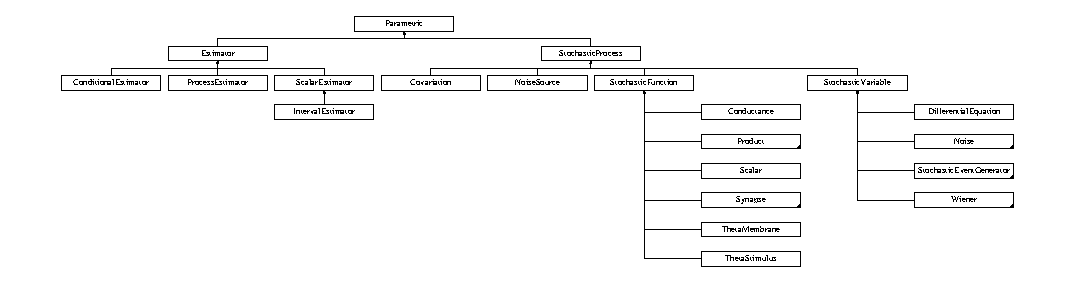
\includegraphics[height=3.35329cm]{classParametric}
\end{center}
\end{figure}


\subsection{Detailed Description}
Class describing objects which can be parametrized. 

Objects of this class (such as stochastic variables) can be parametrized in various ways. A paremeter (const Property\&) is an integer constant which identifies the parameter. \subsection*{Public Member Functions}
\begin{CompactItemize}
\item 
string {\bf getType} ()\label{classParametric_96ec2935d9515d39d535e914673c9888}

\begin{CompactList}\small\item\em Type of object. \item\end{CompactList}\item 
string {\bf getName} ()\label{classParametric_ec30d634a65641c3f372fc6c8922bb56}

\begin{CompactList}\small\item\em Name of object. \item\end{CompactList}\item 
void {\bf setName} (const string \&name)\label{classParametric_b514e8d91defbdb10a70c99fcd411128}

\begin{CompactList}\small\item\em Name of object. \item\end{CompactList}\item 
string {\bf getConfiguration} ()
\begin{CompactList}\small\item\em Returns the configuration of the object. \item\end{CompactList}\item 
string {\bf getAllParameters} ()\label{classParametric_fc22f13591e806ac13fa4750f5cf9f84}

\begin{CompactList}\small\item\em String with all parameter settings. \item\end{CompactList}\item 
void {\bf addParameter} (const string \&name)
\begin{CompactList}\small\item\em Add a parameter. \item\end{CompactList}\item 
void {\bf rmParameter} (const string \&name)
\begin{CompactList}\small\item\em Remove a parameter. \item\end{CompactList}\item 
virtual void {\bf setParameter} (const string \&name, const string \&value)
\begin{CompactList}\small\item\em Set parameter. \item\end{CompactList}\item 
virtual string {\bf getParameter} (const string \&name)
\begin{CompactList}\small\item\em Get parameter. \item\end{CompactList}\end{CompactItemize}
\subsection*{Protected Member Functions}
\begin{CompactItemize}
\item 
{\bf Parametric} (const string \&name, const string \&type)\label{classParametric_417f00c101447dd2e8eca91c40cd6843}

\begin{CompactList}\small\item\em Create object of type and name. \item\end{CompactList}\item 
virtual {\bf $\sim$Parametric} ()\label{classParametric_600bc5f4c9cb58d44aa1f91a72c2caac}

\begin{CompactList}\small\item\em Destroy object. \item\end{CompactList}\end{CompactItemize}


\subsection{Member Function Documentation}
\index{Parametric@{Parametric}!getConfiguration@{getConfiguration}}
\index{getConfiguration@{getConfiguration}!Parametric@{Parametric}}
\subsubsection[getConfiguration]{\setlength{\rightskip}{0pt plus 5cm}string Parametric::getConfiguration ()}\label{classParametric_4ca566f675c36cb40afb68561fd9df3c}


Returns the configuration of the object. 

This includes object type and name, and a list with all settings. \index{Parametric@{Parametric}!addParameter@{addParameter}}
\index{addParameter@{addParameter}!Parametric@{Parametric}}
\subsubsection[addParameter]{\setlength{\rightskip}{0pt plus 5cm}void Parametric::addParameter (const string \& {\em name})}\label{classParametric_d96495ef7f226ec3360bd8971c3bf4de}


Add a parameter. 

Adds another string definition to the class. If the parameter already exists, it is not added. \index{Parametric@{Parametric}!rmParameter@{rmParameter}}
\index{rmParameter@{rmParameter}!Parametric@{Parametric}}
\subsubsection[rmParameter]{\setlength{\rightskip}{0pt plus 5cm}void Parametric::rmParameter (const string \& {\em name})}\label{classParametric_f4b8fa2dd141c55610825f495ed6d542}


Remove a parameter. 

Removes the string from the parameter list. \index{Parametric@{Parametric}!setParameter@{setParameter}}
\index{setParameter@{setParameter}!Parametric@{Parametric}}
\subsubsection[setParameter]{\setlength{\rightskip}{0pt plus 5cm}virtual void Parametric::setParameter (const string \& {\em name}, \/  const string \& {\em value})\hspace{0.3cm}{\tt  [virtual]}}\label{classParametric_bba36dc4545219658541ab55251e02e6}


Set parameter. 

Sets the value of a parameter using strings. If a parameter is described using multiple strings separated by space, this indicates a parameter of a parameter (not implemented yet). \begin{Desc}
\item[Parameters: ]\par
\begin{description}
\item[{\em 
name}]name of parameter \item[{\em 
value}]value of parameter (used with operator$<$$<$) \end{description}
\end{Desc}


Reimplemented in {\bf IfNeuron} \doxyref{}{p.}{classIfNeuron_657741be3d616bd029ff1eab9136247a}, {\bf Noise} \doxyref{}{p.}{classNoise_2dee7f54aab2701376c9500c69f5d5e4}, {\bf Scalar} \doxyref{}{p.}{classScalar_9ec6ab9b6716e798ffc9e6bfed1b19fc}, {\bf Product} \doxyref{}{p.}{classProduct_7009c5b4f1b459230f5754a3675d38de}, {\bf Conductance} \doxyref{}{p.}{classConductance_f554e9cb35c3204747b1ce14a1024893}, {\bf Poisson} \doxyref{}{p.}{classPoisson_6301e62f1bc91eda792bc8d1412f4e1e}, {\bf Synapse} \doxyref{}{p.}{classSynapse_abe8f9af570c03d381475c6e4b5912d7}, {\bf SimpleSynapse} \doxyref{}{p.}{classSimpleSynapse_6a9584eea4c121415068e539d6603783}, {\bf Wiener} \doxyref{}{p.}{classWiener_69c25adbb4bcad391350812d7f59f84c}, and {\bf WienerCpp} \doxyref{}{p.}{classWienerCpp_afdaaadb8175a259d4bc420c823829a0}.\index{Parametric@{Parametric}!getParameter@{getParameter}}
\index{getParameter@{getParameter}!Parametric@{Parametric}}
\subsubsection[getParameter]{\setlength{\rightskip}{0pt plus 5cm}virtual string Parametric::getParameter (const string \& {\em name})\hspace{0.3cm}{\tt  [virtual]}}\label{classParametric_3c39188e1750b8e5d442b9dfa079b1c8}


Get parameter. 

In a derived class, override this to handle every parameter you implement. If a parameter is described using multiple strings separated by space, this indicates a parameter of a parameter. \begin{Desc}
\item[Parameters: ]\par
\begin{description}
\item[{\em 
name}]name of parameter \end{description}
\end{Desc}


Reimplemented in {\bf DifferentialEquation} \doxyref{}{p.}{classDifferentialEquation_8edfa603b974d803268a604dff8ff964}, {\bf IfNeuron} \doxyref{}{p.}{classIfNeuron_a2491c69e51d8d2f93eacf6b2067b192}, {\bf Noise} \doxyref{}{p.}{classNoise_426f116ca5396f47710f604f1085c4fe}, {\bf Scalar} \doxyref{}{p.}{classScalar_1bcc13696ba052e1f15aa3bf6bcf5fc5}, {\bf Product} \doxyref{}{p.}{classProduct_d9c5ec64bd836a6714b76f62e78562a9}, {\bf Conductance} \doxyref{}{p.}{classConductance_e7a8b09fa5096cbf0cb4fd2e08696a63}, {\bf Poisson} \doxyref{}{p.}{classPoisson_f4bf48e6e02c4c72ed43561fc62a1cc2}, {\bf Synapse} \doxyref{}{p.}{classSynapse_8d70e1e7f33cef4e1a1b4d8f504fd4bd}, {\bf SimpleSynapse} \doxyref{}{p.}{classSimpleSynapse_9c88f99370d1349d00c9707f8fa1c7cd}, {\bf Wiener} \doxyref{}{p.}{classWiener_313637cdbd6ae2865897bf48fa1ced4b}, and {\bf WienerCpp} \doxyref{}{p.}{classWienerCpp_6e9dd9a019c621a7990f4133d476c92c}.
\section{Physical Class Reference}
\label{classPhysical}\index{Physical@{Physical}}
Inheritance diagram for Physical::\begin{figure}[H]
\begin{center}
\leavevmode
\includegraphics[height=3.77245cm]{classPhysical}
\end{center}
\end{figure}


\subsection{Detailed Description}
A physical value. 

This is a 'something' that has a physical dimension (like time, weight, length...). It has a physical unit and a name (like 'voltage'). Use physical.getUnit().set(...) to set the physical unit. \subsection*{Public Member Functions}
\begin{CompactItemize}
\item 
{\bf Physical} ()\label{classPhysical_c11a1bca87389886d9d8291fef41ad8c}

\begin{CompactList}\small\item\em Construct. \item\end{CompactList}\item 
{\bf Physical} (const {\bf Physical} \&)\label{classPhysical_7fcd70d51b73aa1a3f87e720d4641b6e}

\begin{CompactList}\small\item\em Copy. \item\end{CompactList}\item 
{\bf Physical} (string name)\label{classPhysical_33a5587060fe65720af0dadb735fb40f}

\begin{CompactList}\small\item\em Construct. \item\end{CompactList}\item 
{\bf Physical} (string name, string unitPrefix, string unitSymbol)\label{classPhysical_458571d306663bf819ca16bbd60cce2f}

\begin{CompactList}\small\item\em Construct. \item\end{CompactList}\item 
{\bf Physical} (string name, {\bf Unit} unit)\label{classPhysical_ed21477e9666fce55fce7e43b47b2287}

\begin{CompactList}\small\item\em Construct. \item\end{CompactList}\item 
virtual string {\bf getDescription} ()
\begin{CompactList}\small\item\em Retriev the name. \item\end{CompactList}\item 
virtual string {\bf getPhysicalDescription} ()
\begin{CompactList}\small\item\em Returns the physical description. \item\end{CompactList}\item 
virtual string {\bf getUnitName} ()\label{classPhysical_359a145863a529b1f7f986865045106b}

\begin{CompactList}\small\item\em Returns the unit name. \item\end{CompactList}\item 
virtual string {\bf getUnitSymbol} ()\label{classPhysical_79d85f6ec2b728ef1f5154105b5003c6}

\begin{CompactList}\small\item\em Returns the unit name. \item\end{CompactList}\item 
virtual void {\bf setDescription} (string name)
\begin{CompactList}\small\item\em Set the name. \item\end{CompactList}\item 
virtual void {\bf setUnit} ({\bf Unit} u)\label{classPhysical_1262a520e80201dad23bc84c322f1eae}

\begin{CompactList}\small\item\em Set the unit. \item\end{CompactList}\item 
virtual void {\bf setUnitPrefix} (int n)
\begin{CompactList}\small\item\em Set unit prefix. \item\end{CompactList}\item 
virtual {\bf Unit} {\bf getUnit} () const \label{classPhysical_57174c2980a2e5ff5e4bf4f0c6450bd6}

\begin{CompactList}\small\item\em Retrieve the unit. \item\end{CompactList}\end{CompactItemize}


\subsection{Member Function Documentation}
\index{Physical@{Physical}!getDescription@{getDescription}}
\index{getDescription@{getDescription}!Physical@{Physical}}
\subsubsection[getDescription]{\setlength{\rightskip}{0pt plus 5cm}virtual string Physical::getDescription ()\hspace{0.3cm}{\tt  [virtual]}}\label{classPhysical_e01f498fa44a20cabcc1a1b723551514}


Retriev the name. 

The name is constructed from the physical name (like \char`\"{}membrane voltage\char`\"{}) and the unit symbol (like \char`\"{}mV\char`\"{}). In this example is would read \char`\"{}membrane voltage [mV]\char`\"{}. 

Reimplemented in {\bf StochasticProcess} \doxyref{}{p.}{classStochasticProcess_dcb7c542f6cbc5fafef7d80ce39b0cd3}.\index{Physical@{Physical}!getPhysicalDescription@{getPhysicalDescription}}
\index{getPhysicalDescription@{getPhysicalDescription}!Physical@{Physical}}
\subsubsection[getPhysicalDescription]{\setlength{\rightskip}{0pt plus 5cm}virtual string Physical::getPhysicalDescription ()\hspace{0.3cm}{\tt  [inline, virtual]}}\label{classPhysical_fae32a308991e05f2e5444f6af8f877f}


Returns the physical description. 

This is the name of the physical dimension of the object, if it has any. (\char`\"{}\char`\"{} otherwise) 

Reimplemented in {\bf Time} \doxyref{}{p.}{classTime_1ac1a866153ab2dd80abf20b6e923909}.\index{Physical@{Physical}!setDescription@{setDescription}}
\index{setDescription@{setDescription}!Physical@{Physical}}
\subsubsection[setDescription]{\setlength{\rightskip}{0pt plus 5cm}virtual void Physical::setDescription (string {\em name})\hspace{0.3cm}{\tt  [virtual]}}\label{classPhysical_9acbf2eae3b93d0073003b8603afda98}


Set the name. 

The name of the physical quantity, like 'voltage' 

Reimplemented in {\bf StochasticProcess} \doxyref{}{p.}{classStochasticProcess_0365e8bce98c851e72220282477e62a5}.\index{Physical@{Physical}!setUnitPrefix@{setUnitPrefix}}
\index{setUnitPrefix@{setUnitPrefix}!Physical@{Physical}}
\subsubsection[setUnitPrefix]{\setlength{\rightskip}{0pt plus 5cm}virtual void Physical::setUnitPrefix (int {\em n})\hspace{0.3cm}{\tt  [virtual]}}\label{classPhysical_ee82aa27916708a2290415dc9e822e59}


Set unit prefix. 

Set the unit prefix by giving an integer from -24 to 24. Should be a multiple of 3, exception: -2,-1,2,1. 
\section{Plot Class Reference}
\label{classPlot}\index{Plot@{Plot}}


\subsection{Detailed Description}
A plot descriptor used by the \doxyref{Display}{p.}{classDisplay} class. 

This is meant to be used internally by the \doxyref{Display}{p.}{classDisplay} class. An object like this describes a plot command in gnuplot. \subsection*{Public Member Functions}
\begin{CompactItemize}
\item 
{\bf Plot} (string function, string name, string xlabel, string ylabel, string zlabel, int mode, int lineStyle=0)\label{classPlot_e6775a6ea2fb75111e4e1214248a498d}

\begin{CompactList}\small\item\em Construct. \item\end{CompactList}\item 
{\bf $\sim$Plot} ()\label{classPlot_277e9c79c4357b3a317d74d61dabefcf}

\begin{CompactList}\small\item\em Destruct. \item\end{CompactList}\end{CompactItemize}
\subsection*{Public Attributes}
\begin{CompactItemize}
\item 
string {\bf sFunction}\label{classPlot_e0e45513ab4e5f61ff5dcd9907df7230}

\begin{CompactList}\small\item\em The function (analytic expression or filename). \item\end{CompactList}\item 
string {\bf sName}\label{classPlot_21a57ca64b6453bd6d9fef4d9246a6bf}

\begin{CompactList}\small\item\em The name (label in gnuplot). \item\end{CompactList}\item 
int {\bf nMode}\label{classPlot_baf8a3f7041264517e4d88eb243db299}

\begin{CompactList}\small\item\em The mode (2D, 3D etc.). \item\end{CompactList}\item 
string {\bf sXLabel}\label{classPlot_aada51b50fd979d22a9ee4b59d694656}

\begin{CompactList}\small\item\em The x-axis label. \item\end{CompactList}\item 
string {\bf sYLabel}\label{classPlot_e80b3b22eeab37a43f4279d258903da8}

\begin{CompactList}\small\item\em The y-axis label. \item\end{CompactList}\item 
string {\bf sZLabel}\label{classPlot_5cab43c77d4e09a29fffc43acbebd35d}

\begin{CompactList}\small\item\em The z-axis label. \item\end{CompactList}\item 
string {\bf sUserSettings}\label{classPlot_76c298215919d5cd6c4086bdcb6b67ee}

\begin{CompactList}\small\item\em optional user settings \item\end{CompactList}\item 
int {\bf nLineStyle}\label{classPlot_2235afbae6af0379d0790507a093a5c4}

\begin{CompactList}\small\item\em the line type (0 - normal count, 1 - ..: special colour/style) \item\end{CompactList}\end{CompactItemize}

\section{Poisson Class Reference}
\label{classPoisson}\index{Poisson@{Poisson}}
Inheritance diagram for Poisson::\begin{figure}[H]
\begin{center}
\leavevmode
\includegraphics[height=5cm]{classPoisson}
\end{center}
\end{figure}


\subsection{Detailed Description}
Returns delta peaks with a static rate. 

\doxyref{Poisson}{p.}{classPoisson} process: steps forward when using either () or (double) operators. \subsection*{Public Member Functions}
\begin{CompactItemize}
\item 
{\bf Poisson} (double p, {\bf Time} $\ast$time)\label{classPoisson_df4004254b44c3ef3d990abdcd1d0e55}

\begin{CompactList}\small\item\em Create \doxyref{Poisson}{p.}{classPoisson} process. \item\end{CompactList}\item 
{\bf $\sim$Poisson} ()\label{classPoisson_dc599dacb253169758ed80a609917545}

\begin{CompactList}\small\item\em Destroy \doxyref{Poisson}{p.}{classPoisson} process. \item\end{CompactList}\item 
virtual bool {\bf hasEvent} ()\label{classPoisson_681289876ddd558bccb9bc501553cc62}

\begin{CompactList}\small\item\em Whether event is present. \item\end{CompactList}\item 
virtual void {\bf prepareNextState} ()\label{classPoisson_080ccca540e025812d091fdae3b4075c}

\begin{CompactList}\small\item\em Calculate next time value. \item\end{CompactList}\item 
virtual string {\bf getParameter} (const string \&name)\label{classPoisson_f4bf48e6e02c4c72ed43561fc62a1cc2}

\begin{CompactList}\small\item\em Get parameter. \item\end{CompactList}\item 
virtual void {\bf setParameter} (const string \&name, const string \&value)\label{classPoisson_6301e62f1bc91eda792bc8d1412f4e1e}

\begin{CompactList}\small\item\em Set parameter. \item\end{CompactList}\end{CompactItemize}

\section{PoissonNoise Class Reference}
\label{classPoissonNoise}\index{PoissonNoise@{PoissonNoise}}
Inheritance diagram for PoissonNoise::\begin{figure}[H]
\begin{center}
\leavevmode
\includegraphics[height=5cm]{classPoissonNoise}
\end{center}
\end{figure}


\subsection{Detailed Description}
A poisson noise source. 

Internal class: You never need to acces this class directly, since all public members are defined in \doxyref{Noise}{p.}{classNoise}. This special derivation of \doxyref{Noise}{p.}{classNoise} is only important internally, for the \doxyref{NoiseSource}{p.}{classNoiseSource} class. \subsection*{Public Member Functions}
\begin{CompactItemize}
\item 
virtual {\bf Noise} \& {\bf setWeight} (double w)\label{classPoissonNoise_5d1a2dfe8e7d42f110cad707ec042c31}

\begin{CompactList}\small\item\em Set the weight. \item\end{CompactList}\item 
virtual {\bf Noise} \& {\bf setRate} (double r)\label{classPoissonNoise_e664147545fe4be392dac717299c1da1}

\begin{CompactList}\small\item\em Set the rate. \item\end{CompactList}\item 
virtual {\bf Noise} \& {\bf setMean} (double m)\label{classPoissonNoise_07a0dcd7dddadc6235e47b81029182b7}

\begin{CompactList}\small\item\em Set the mean. \item\end{CompactList}\item 
virtual {\bf Noise} \& {\bf setStdDev} (double s)\label{classPoissonNoise_cace326336128b6214dd962bd94df5c1}

\begin{CompactList}\small\item\em Set the standard deviation coefficient. \item\end{CompactList}\end{CompactItemize}
\subsection*{Protected Member Functions}
\begin{CompactItemize}
\item 
{\bf PoissonNoise} (class {\bf NoiseSource} $\ast$, int index, const string \&name=\char`\"{}\char`\"{}, const string \&type=\char`\"{}correlated\_\-poisson\_\-process\char`\"{})
\begin{CompactList}\small\item\em Construct. \item\end{CompactList}\item 
{\bf PoissonNoise} (const {\bf PoissonNoise} \&)
\begin{CompactList}\small\item\em Construct. \item\end{CompactList}\item 
virtual void {\bf setNext} (double indicator)
\begin{CompactList}\small\item\em Set the next values. \item\end{CompactList}\end{CompactItemize}
\subsection*{Friends}
\begin{CompactItemize}
\item 
class {\bf NoiseSource}\label{classPoissonNoise_14268df5638debed66cad6d85946916f}

\end{CompactItemize}


\subsection{Constructor \& Destructor Documentation}
\index{PoissonNoise@{PoissonNoise}!PoissonNoise@{PoissonNoise}}
\index{PoissonNoise@{PoissonNoise}!PoissonNoise@{PoissonNoise}}
\subsubsection[PoissonNoise]{\setlength{\rightskip}{0pt plus 5cm}PoissonNoise::PoissonNoise (class {\bf NoiseSource} $\ast$, \/  int {\em index}, \/  const string \& {\em name} = {\tt \char`\"{}\char`\"{}}, \/  const string \& {\em type} = {\tt \char`\"{}correlated\_\-poisson\_\-process\char`\"{}})\hspace{0.3cm}{\tt  [protected]}}\label{classPoissonNoise_7c3aa407c2848c8c332b0a838466233e}


Construct. 

This constructor is protected, because this class can only be instantiated by calls from the \doxyref{NoiseSource}{p.}{classNoiseSource} class. \index{PoissonNoise@{PoissonNoise}!PoissonNoise@{PoissonNoise}}
\index{PoissonNoise@{PoissonNoise}!PoissonNoise@{PoissonNoise}}
\subsubsection[PoissonNoise]{\setlength{\rightskip}{0pt plus 5cm}PoissonNoise::PoissonNoise (const {\bf PoissonNoise} \&)\hspace{0.3cm}{\tt  [protected]}}\label{classPoissonNoise_327ad60e2915cbbe5676beeb800618ce}


Construct. 

This class mustn't be copied. 

\subsection{Member Function Documentation}
\index{PoissonNoise@{PoissonNoise}!setNext@{setNext}}
\index{setNext@{setNext}!PoissonNoise@{PoissonNoise}}
\subsubsection[setNext]{\setlength{\rightskip}{0pt plus 5cm}virtual void PoissonNoise::setNext (double {\em indicator})\hspace{0.3cm}{\tt  [protected, virtual]}}\label{classPoissonNoise_152fad5631c941cb7a6b333da961d69a}


Set the next values. 

The main method. The \doxyref{NoiseSource}{p.}{classNoiseSource} class uses this to set the indicator values. If the indicator is above the current threshold, the value is set to w (the weight of the process), otherwise to 0.0. 

Implements {\bf Noise} \doxyref{}{p.}{classNoise}.
\section{ProcessEstimator Class Reference}
\label{classProcessEstimator}\index{ProcessEstimator@{ProcessEstimator}}
Inheritance diagram for ProcessEstimator::\begin{figure}[H]
\begin{center}
\leavevmode
\includegraphics[height=3cm]{classProcessEstimator}
\end{center}
\end{figure}


\subsection{Detailed Description}
Estimates mean, var, etc. of a stochastic process. 

Records a sample from a given process from the start for a given time period. After that period, recording is stopped, until \doxyref{init()}{p.}{classProcessEstimator_29033f5d95a263708516c08c16b61f78} is called. This is useful, when the beginning of processes has to be estimated, and these processes are not events. \subsection*{Public Member Functions}
\begin{CompactItemize}
\item 
virtual void {\bf init} ()\label{classProcessEstimator_29033f5d95a263708516c08c16b61f78}

\begin{CompactList}\small\item\em initialise to take next process sample \item\end{CompactList}\item 
virtual void {\bf collect} ()\label{classProcessEstimator_c13f0d356e07023d8456298f78db5124}

\begin{CompactList}\small\item\em receive next data point \item\end{CompactList}\item 
virtual {\bf Matrix} {\bf mResult} (const Property \&)\label{classProcessEstimator_1025419b6147354d3bae12429db53643}

\begin{CompactList}\small\item\em get a property \item\end{CompactList}\item 
{\bf ProcessEstimator} (const Property \&, {\bf StochasticProcess} $\ast$, {\bf Time} $\ast$, int length)\label{classProcessEstimator_a80b8448e3b3c1669b4e89e5a3c59623}

\begin{CompactList}\small\item\em construct \item\end{CompactList}\item 
virtual {\bf $\sim$ProcessEstimator} ()\label{classProcessEstimator_f288bdb208457b07923d027a2b8c039c}

\begin{CompactList}\small\item\em destruct \item\end{CompactList}\end{CompactItemize}

\section{Product Class Reference}
\label{classProduct}\index{Product@{Product}}
Inheritance diagram for Product::\begin{figure}[H]
\begin{center}
\leavevmode
\includegraphics[height=5cm]{classProduct}
\end{center}
\end{figure}


\subsection{Detailed Description}
A product of the function input and a scalar. \subsection*{Public Member Functions}
\begin{CompactItemize}
\item 
{\bf Product} (double factor, const string \&name=\char`\"{}\char`\"{}, const string \&type=\char`\"{}product\char`\"{})\label{classProduct_b8605181d2afd73bd3ec6c043d017326}

\begin{CompactList}\small\item\em Create. \item\end{CompactList}\item 
virtual {\bf $\sim$Product} ()\label{classProduct_18f26095e25405579968c6ede367484f}

\begin{CompactList}\small\item\em Destroy. \item\end{CompactList}\item 
virtual double {\bf calculateCurrentValue} ()\label{classProduct_f54c958e082fa36cde289a09a6ba9765}

\begin{CompactList}\small\item\em Return current product value. \item\end{CompactList}\item 
virtual double {\bf calculateNextValue} ()\label{classProduct_d8fae226e9ad34bc3ed33dd294fd7186}

\begin{CompactList}\small\item\em Return next product value. \item\end{CompactList}\item 
virtual string {\bf getParameter} (const string \&name)
\begin{CompactList}\small\item\em Get parameter. \item\end{CompactList}\item 
virtual void {\bf setParameter} (const string \&name, const string \&value)
\begin{CompactList}\small\item\em Set parameter. \item\end{CompactList}\end{CompactItemize}


\subsection{Member Function Documentation}
\index{Product@{Product}!getParameter@{getParameter}}
\index{getParameter@{getParameter}!Product@{Product}}
\subsubsection[getParameter]{\setlength{\rightskip}{0pt plus 5cm}virtual string Product::getParameter (const string \& {\em name})\hspace{0.3cm}{\tt  [virtual]}}\label{classProduct_d9c5ec64bd836a6714b76f62e78562a9}


Get parameter. 

Implements \char`\"{}value\char`\"{}. 

Reimplemented from {\bf Parametric} \doxyref{}{p.}{classParametric_3c39188e1750b8e5d442b9dfa079b1c8}.\index{Product@{Product}!setParameter@{setParameter}}
\index{setParameter@{setParameter}!Product@{Product}}
\subsubsection[setParameter]{\setlength{\rightskip}{0pt plus 5cm}virtual void Product::setParameter (const string \& {\em name}, \/  const string \& {\em value})\hspace{0.3cm}{\tt  [virtual]}}\label{classProduct_7009c5b4f1b459230f5754a3675d38de}


Set parameter. 

Implements \char`\"{}value\char`\"{}. 

Reimplemented from {\bf Parametric} \doxyref{}{p.}{classParametric_bba36dc4545219658541ab55251e02e6}.
\section{Queue$<$ T $>$ Class Template Reference}
\label{classQueue}\index{Queue@{Queue}}
Inherits Ring$<$ T $>$.



\subsection{Detailed Description}
\subsubsection*{template$<$typename T$>$ class Queue$<$ T $>$}

Small queue. 

Class for storing basic data types in a simple queue. Push and pop work via $<$$<$ and $>$$>$, and += is defined. If you want something better, use the STL queue. 
\section{RandN Class Reference}
\label{classRandN}\index{RandN@{RandN}}
Inheritance diagram for RandN::\begin{figure}[H]
\begin{center}
\leavevmode
\includegraphics[height=3cm]{classRandN}
\end{center}
\end{figure}


\subsection{Detailed Description}
An object which uses the randn function. 

This class implements a random variable with normal distribution (gaussian). \subsection*{Public Member Functions}
\begin{CompactItemize}
\item 
{\bf RandN} ()\label{classRandN_e842af49a10a6dc84bdcf2a0cc643f98}

\begin{CompactList}\small\item\em Construct. \item\end{CompactList}\item 
{\bf $\sim$RandN} ()\label{classRandN_ffb47d3d5cb0d2c28e4d7b84f5ee81ff}

\begin{CompactList}\small\item\em Destruct. \item\end{CompactList}\item 
double {\bf dRandN} ()
\begin{CompactList}\small\item\em Retrieve random variable. \item\end{CompactList}\end{CompactItemize}


\subsection{Member Function Documentation}
\index{RandN@{RandN}!dRandN@{dRandN}}
\index{dRandN@{dRandN}!RandN@{RandN}}
\subsubsection[dRandN]{\setlength{\rightskip}{0pt plus 5cm}double RandN::dRandN ()}\label{classRandN_0f821b3a122bbd285978503e504bd5f8}


Retrieve random variable. 

This function generates one random variable. The returend values are normally (Gaussian) distributed, with a mean of 0.0 and a variance of 1.0. The method used is the Polar-Masaglia method, which is the quickest known so far. 
\section{Scalar Class Reference}
\label{classScalar}\index{Scalar@{Scalar}}
Inheritance diagram for Scalar::\begin{figure}[H]
\begin{center}
\leavevmode
\includegraphics[height=4cm]{classScalar}
\end{center}
\end{figure}


\subsection{Detailed Description}
returns a scalar \subsection*{Public Member Functions}
\begin{CompactItemize}
\item 
{\bf Scalar} (double scalar, const string \&name, const string \&type=\char`\"{}scalar\char`\"{})
\begin{CompactList}\small\item\em Construct. \item\end{CompactList}\item 
{\bf Scalar} (double scalar, string unitPrefix, string unitSymbol, const string \&name, const string \&type=\char`\"{}scalar\char`\"{})
\begin{CompactList}\small\item\em Construct. \item\end{CompactList}\item 
virtual {\bf $\sim$Scalar} ()\label{classScalar_e2bcc0c8af86161e9220cc68d1f85d29}

\begin{CompactList}\small\item\em Destroy. \item\end{CompactList}\item 
virtual string {\bf getParameter} (const string \&name)
\begin{CompactList}\small\item\em Get parameter. \item\end{CompactList}\item 
virtual void {\bf setParameter} (const string \&name, const string \&value)
\begin{CompactList}\small\item\em Set parameter. \item\end{CompactList}\item 
virtual double {\bf calculateCurrentValue} ()\label{classScalar_cca9680da905b4fb1e3a4b2bbe527417}

\begin{CompactList}\small\item\em Calculates the current value based on the current input. \item\end{CompactList}\item 
virtual double {\bf calculateNextValue} ()\label{classScalar_0aab66e2480c065282c78c52cab3a28b}

\begin{CompactList}\small\item\em Calculates the next value based on the current input. \item\end{CompactList}\end{CompactItemize}


\subsection{Constructor \& Destructor Documentation}
\index{Scalar@{Scalar}!Scalar@{Scalar}}
\index{Scalar@{Scalar}!Scalar@{Scalar}}
\subsubsection[Scalar]{\setlength{\rightskip}{0pt plus 5cm}Scalar::Scalar (double {\em scalar}, \/  const string \& {\em name}, \/  const string \& {\em type} = {\tt \char`\"{}scalar\char`\"{}})}\label{classScalar_2245b31a3fc102f905acb308bde35c01}


Construct. 

Construct a scalar with a description. \index{Scalar@{Scalar}!Scalar@{Scalar}}
\index{Scalar@{Scalar}!Scalar@{Scalar}}
\subsubsection[Scalar]{\setlength{\rightskip}{0pt plus 5cm}Scalar::Scalar (double {\em scalar}, \/  string {\em unitPrefix}, \/  string {\em unitSymbol}, \/  const string \& {\em name}, \/  const string \& {\em type} = {\tt \char`\"{}scalar\char`\"{}})}\label{classScalar_bc1c7c294a9143c2d940c6d365f57bfe}


Construct. 

Construcr a scalar with a description and a physical unit. 

\subsection{Member Function Documentation}
\index{Scalar@{Scalar}!getParameter@{getParameter}}
\index{getParameter@{getParameter}!Scalar@{Scalar}}
\subsubsection[getParameter]{\setlength{\rightskip}{0pt plus 5cm}virtual string Scalar::getParameter (const string \& {\em name})\hspace{0.3cm}{\tt  [virtual]}}\label{classScalar_1bcc13696ba052e1f15aa3bf6bcf5fc5}


Get parameter. 

Implements \char`\"{}value\char`\"{}. 

Reimplemented from {\bf Parametric} \doxyref{}{p.}{classParametric_3c39188e1750b8e5d442b9dfa079b1c8}.\index{Scalar@{Scalar}!setParameter@{setParameter}}
\index{setParameter@{setParameter}!Scalar@{Scalar}}
\subsubsection[setParameter]{\setlength{\rightskip}{0pt plus 5cm}virtual void Scalar::setParameter (const string \& {\em name}, \/  const string \& {\em value})\hspace{0.3cm}{\tt  [virtual]}}\label{classScalar_9ec6ab9b6716e798ffc9e6bfed1b19fc}


Set parameter. 

Implements \char`\"{}value\char`\"{}. 

Reimplemented from {\bf Parametric} \doxyref{}{p.}{classParametric_bba36dc4545219658541ab55251e02e6}.
\section{ScalarEstimator Class Reference}
\label{classScalarEstimator}\index{ScalarEstimator@{ScalarEstimator}}
Inheritance diagram for ScalarEstimator::\begin{figure}[H]
\begin{center}
\leavevmode
\includegraphics[height=4cm]{classScalarEstimator}
\end{center}
\end{figure}


\subsection{Detailed Description}
estimates mean, variance, etc. of a scalar stochastic variable \subsection*{Public Member Functions}
\begin{CompactItemize}
\item 
virtual void {\bf collect} ()\label{classScalarEstimator_fa275bacad14fae90cf403d42034112a}

\begin{CompactList}\small\item\em Eat next piece of data. \item\end{CompactList}\item 
virtual void {\bf init} ()\label{classScalarEstimator_8d86d47438a830cdf232565f69c178ae}

\begin{CompactList}\small\item\em reset all values \item\end{CompactList}\item 
virtual {\bf Matrix} {\bf mResult} (const Property \&)\label{classScalarEstimator_0b89bead8f660dc70a29f27c04a84211}

\begin{CompactList}\small\item\em return result of estimation \item\end{CompactList}\item 
{\bf ScalarEstimator} (const Property \&, {\bf StochasticProcess} $\ast$, {\bf Time} $\ast$)\label{classScalarEstimator_fe3a8e544172fa276c63404f9568e5a8}

\begin{CompactList}\small\item\em Constructor. \item\end{CompactList}\item 
void {\bf setProperty} (const Property \&, double)\label{classScalarEstimator_b6f834caacc81731a3ac8680f4ef133f}

\begin{CompactList}\small\item\em set distribution-related properties \item\end{CompactList}\item 
virtual {\bf $\sim$ScalarEstimator} ()\label{classScalarEstimator_47ce0d225e027640e8bc27488917cd59}

\begin{CompactList}\small\item\em Destructor. \item\end{CompactList}\end{CompactItemize}

\section{SimpleSynapse Class Reference}
\label{classSimpleSynapse}\index{SimpleSynapse@{SimpleSynapse}}
Inheritance diagram for SimpleSynapse::\begin{figure}[H]
\begin{center}
\leavevmode
\includegraphics[height=5cm]{classSimpleSynapse}
\end{center}
\end{figure}


\subsection{Detailed Description}
A synapse. 

This class implements a synapse which is characterized by a differential equation. Main feature is the transformation of digital signals from an Event object (usually a neuron) to analog values of a \doxyref{StochasticProcess}{p.}{classStochasticProcess} object, which then are part of the membrane equation of another neuron. It also possible to use a noise source (such as a \doxyref{Wiener}{p.}{classWiener} process) as input. This depends on the constructor you use. Since a synapse usually connects from one single neuron to another single neuron, this class is set to be active as default, i.e. is forwarded automatically and you don't have to use \doxyref{proceedToNextState()}{p.}{classSimpleSynapse_af49bacea075b5b2d4824a348ee2ecb2} and \doxyref{prepareNextState()}{p.}{classSimpleSynapse_4a737cab949dbf6c74e4990f7d7daeca} inside your program. \subsection*{Public Member Functions}
\begin{CompactItemize}
\item 
{\bf SimpleSynapse} ({\bf Time} $\ast$time, {\bf StochasticEventGenerator} $\ast$e, double weight, double revPot, double peak, double tau)
\begin{CompactList}\small\item\em Construct. \item\end{CompactList}\item 
{\bf SimpleSynapse} ({\bf Time} $\ast$time, {\bf StochasticVariable} $\ast$s, double weight, double revPot, double tau)
\begin{CompactList}\small\item\em Construct. \item\end{CompactList}\item 
virtual void {\bf prepareNextState} ()\label{classSimpleSynapse_4a737cab949dbf6c74e4990f7d7daeca}

\begin{CompactList}\small\item\em Calculate next state. \item\end{CompactList}\item 
virtual void {\bf proceedToNextState} ()\label{classSimpleSynapse_af49bacea075b5b2d4824a348ee2ecb2}

\begin{CompactList}\small\item\em Apply nex time step. \item\end{CompactList}\item 
virtual double {\bf calculateNextValue} ()\label{classSimpleSynapse_4753862000caa1957f572325644e9780}

\begin{CompactList}\small\item\em Calculate next value. \item\end{CompactList}\item 
virtual double {\bf calculateCurrentValue} ()\label{classSimpleSynapse_519447f6b2f414f9e6ec6475808fda15}

\begin{CompactList}\small\item\em Calculate current value. \item\end{CompactList}\item 
{\bf $\sim$SimpleSynapse} ()\label{classSimpleSynapse_bb981be345280d99d0634549b1b7b5fa}

\begin{CompactList}\small\item\em Destruct. \item\end{CompactList}\item 
virtual void {\bf setParameter} (const string \&name, const string \&value)
\begin{CompactList}\small\item\em Set parameter. \item\end{CompactList}\item 
virtual string {\bf getParameter} (const string \&name)
\begin{CompactList}\small\item\em Get parameter. \item\end{CompactList}\end{CompactItemize}
\subsection*{Protected Attributes}
\begin{CompactItemize}
\item 
{\bf DifferentialEquation} {\bf differential}
\begin{CompactList}\small\item\em Differential equation. \item\end{CompactList}\item 
{\bf StochasticVariable} $\ast$ {\bf stochastic}
\begin{CompactList}\small\item\em \doxyref{Noise}{p.}{classNoise} source. \item\end{CompactList}\end{CompactItemize}


\subsection{Constructor \& Destructor Documentation}
\index{SimpleSynapse@{SimpleSynapse}!SimpleSynapse@{SimpleSynapse}}
\index{SimpleSynapse@{SimpleSynapse}!SimpleSynapse@{SimpleSynapse}}
\subsubsection[SimpleSynapse]{\setlength{\rightskip}{0pt plus 5cm}SimpleSynapse::SimpleSynapse ({\bf Time} $\ast$ {\em time}, \/  {\bf StochasticEventGenerator} $\ast$ {\em e}, \/  double {\em weight}, \/  double {\em revPot}, \/  double {\em peak}, \/  double {\em tau})}\label{classSimpleSynapse_9a0eb5672f207026418a1b072bcd0d75}


Construct. 

Will construct a synapse, which will set its value to the peak conductance just after the pre-synaptic spike, and decay the value according to the given time constant. At the next pre-synaptic spike the value will be set to the peak conductance again. \begin{Desc}
\item[Parameters: ]\par
\begin{description}
\item[{\em 
time}]pointer to main time object \item[{\em 
e}]The object providing the events (spikes), i.e. the pre-synaptic neuron. \item[{\em 
weight}]Weight of the synapse. \item[{\em 
revPot}]Reversal potential of synapse. \item[{\em 
peak}]Peak conductance of synapse. \item[{\em 
tau}]Decay time constant. \end{description}
\end{Desc}
\index{SimpleSynapse@{SimpleSynapse}!SimpleSynapse@{SimpleSynapse}}
\index{SimpleSynapse@{SimpleSynapse}!SimpleSynapse@{SimpleSynapse}}
\subsubsection[SimpleSynapse]{\setlength{\rightskip}{0pt plus 5cm}SimpleSynapse::SimpleSynapse ({\bf Time} $\ast$ {\em time}, \/  {\bf StochasticVariable} $\ast$ {\em s}, \/  double {\em weight}, \/  double {\em revPot}, \/  double {\em tau})}\label{classSimpleSynapse_91d71de8828c8ce87fbbe703053ed4eb}


Construct. 

Will construct a synapse, which will set its value to the peak conductance just after the pre-synaptic spike, and decay the value according to the given time constant. At the next pre-synaptic spike the value will be set to the peak conductance again. \begin{Desc}
\item[Parameters: ]\par
\begin{description}
\item[{\em 
time}]pointer to main time object \item[{\em 
s}]The object providing the stimulus. \item[{\em 
weight}]Weight of the synapse. \item[{\em 
revPot}]Reversal potential of synapse. \item[{\em 
tau}]Decay time constant. \end{description}
\end{Desc}


\subsection{Member Function Documentation}
\index{SimpleSynapse@{SimpleSynapse}!setParameter@{setParameter}}
\index{setParameter@{setParameter}!SimpleSynapse@{SimpleSynapse}}
\subsubsection[setParameter]{\setlength{\rightskip}{0pt plus 5cm}virtual void SimpleSynapse::setParameter (const string \& {\em name}, \/  const string \& {\em value})\hspace{0.3cm}{\tt  [virtual]}}\label{classSimpleSynapse_6a9584eea4c121415068e539d6603783}


Set parameter. 

Sets the value of a parameter using strings. If a parameter is described using multiple strings separated by space, this indicates a parameter of a parameter. \begin{Desc}
\item[Parameters: ]\par
\begin{description}
\item[{\em 
name}]name of parameter \item[{\em 
value}]value of parameter (used with operator$<$$<$) \end{description}
\end{Desc}


Reimplemented from {\bf Synapse} \doxyref{}{p.}{classSynapse_abe8f9af570c03d381475c6e4b5912d7}.\index{SimpleSynapse@{SimpleSynapse}!getParameter@{getParameter}}
\index{getParameter@{getParameter}!SimpleSynapse@{SimpleSynapse}}
\subsubsection[getParameter]{\setlength{\rightskip}{0pt plus 5cm}virtual string SimpleSynapse::getParameter (const string \& {\em name})\hspace{0.3cm}{\tt  [virtual]}}\label{classSimpleSynapse_9c88f99370d1349d00c9707f8fa1c7cd}


Get parameter. 

In a derived class, override this to handle every parameter you implement. If a parameter is described using multiple strings separated by space, this indicates a parameter of a parameter. \begin{Desc}
\item[Parameters: ]\par
\begin{description}
\item[{\em 
name}]name of parameter \end{description}
\end{Desc}


Reimplemented from {\bf Synapse} \doxyref{}{p.}{classSynapse_8d70e1e7f33cef4e1a1b4d8f504fd4bd}.

\subsection{Member Data Documentation}
\index{SimpleSynapse@{SimpleSynapse}!differential@{differential}}
\index{differential@{differential}!SimpleSynapse@{SimpleSynapse}}
\subsubsection[differential]{\setlength{\rightskip}{0pt plus 5cm}{\bf DifferentialEquation} {\bf SimpleSynapse::differential}\hspace{0.3cm}{\tt  [protected]}}\label{classSimpleSynapse_62f65ca9d7e8c3b6d28d760ee4655907}


Differential equation. 

The rate equation. \index{SimpleSynapse@{SimpleSynapse}!stochastic@{stochastic}}
\index{stochastic@{stochastic}!SimpleSynapse@{SimpleSynapse}}
\subsubsection[stochastic]{\setlength{\rightskip}{0pt plus 5cm}{\bf StochasticVariable}$\ast$ {\bf SimpleSynapse::stochastic}\hspace{0.3cm}{\tt  [protected]}}\label{classSimpleSynapse_7e8b5ba04e34caac789ca71278636c14}


\doxyref{Noise}{p.}{classNoise} source. 

only used when the noise constructor was used 
\section{Square Class Reference}
\label{classSquare}\index{Square@{Square}}
Inheritance diagram for Square::\begin{figure}[H]
\begin{center}
\leavevmode
\includegraphics[height=5cm]{classSquare}
\end{center}
\end{figure}


\subsection{Detailed Description}
returns the product of Xt$\ast$Xt and a scalar \subsection*{Public Member Functions}
\begin{CompactItemize}
\item 
virtual double {\bf calculateNextValue} ()\label{classSquare_b03010f31f1716e6ca06c05ad2442c95}

\begin{CompactList}\small\item\em Returns the value at the next time step. \item\end{CompactList}\item 
virtual double {\bf calculateCurrentValue} ()\label{classSquare_1235e02863dad7becef8e8fe04050e66}

\begin{CompactList}\small\item\em Returns the value at the current time step. \item\end{CompactList}\end{CompactItemize}

\section{StochasticEventGenerator Class Reference}
\label{classStochasticEventGenerator}\index{StochasticEventGenerator@{StochasticEventGenerator}}
Inheritance diagram for StochasticEventGenerator::\begin{figure}[H]
\begin{center}
\leavevmode
\includegraphics[height=5cm]{classStochasticEventGenerator}
\end{center}
\end{figure}


\subsection{Detailed Description}
An object which generates events. 

Useful for event-triggered averages. \subsection*{Public Member Functions}
\begin{CompactItemize}
\item 
{\bf StochasticEventGenerator} (class {\bf Time} $\ast$time, const string \&name=\char`\"{}\char`\"{}, const string \&type=\char`\"{}event\_\-generator\char`\"{})\label{classStochasticEventGenerator_f113f0914087df33485ec999204037c6}

\begin{CompactList}\small\item\em Create. \item\end{CompactList}\item 
virtual {\bf $\sim$StochasticEventGenerator} ()\label{classStochasticEventGenerator_fd363097980a3d600520e934b9fdfb1c}

\begin{CompactList}\small\item\em Destroy. \item\end{CompactList}\item 
virtual bool {\bf hasEvent} ()\label{classStochasticEventGenerator_25b18204e3b8f826ed0b0b5b9a4c755a}

\begin{CompactList}\small\item\em Whether an event is present. \item\end{CompactList}\end{CompactItemize}

\section{StochasticFunction Class Reference}
\label{classStochasticFunction}\index{StochasticFunction@{StochasticFunction}}
Inheritance diagram for StochasticFunction::\begin{figure}[H]
\begin{center}
\leavevmode
\includegraphics[height=3.67454cm]{classStochasticFunction}
\end{center}
\end{figure}


\subsection{Detailed Description}
A parametrized stochastic variable. 

Any function which receives a stochastic variable as input, or has some inherent stochastic behaviour, should derive from this class. The members stochCurrentValue and stochNextValue are used for the input to the function. Deriving classes must proved \doxyref{calculateCurrentValue()}{p.}{classStochasticFunction_58551585df52e82ba5b653b17a61bc25}, which returns the value based on stochCurrentValue, and \doxyref{calculateNextValue()}{p.}{classStochasticFunction_8cbed92a69d44112ff269da5b4fa7420}, which returns the the value based on stochNextValue. \subsection*{Public Member Functions}
\begin{CompactItemize}
\item 
{\bf StochasticFunction} (class {\bf Time} $\ast$time, const string \&name=\char`\"{}\char`\"{}, const string \&type=\char`\"{}stochastic\_\-function\char`\"{})\label{classStochasticFunction_a8bb66a782a75a12b68f1b48a955aa51}

\begin{CompactList}\small\item\em Create. \item\end{CompactList}\item 
double {\bf operator()} (double x)
\begin{CompactList}\small\item\em Returns the value at the current time step. \item\end{CompactList}\item 
double {\bf d} (double x)
\begin{CompactList}\small\item\em Returns the increment at the current time step. \item\end{CompactList}\item 
virtual double {\bf getCurrentValue} (double x)
\begin{CompactList}\small\item\em Returns the value at the next time step. \item\end{CompactList}\item 
virtual double {\bf getNextValue} (double x)
\begin{CompactList}\small\item\em Returns the value at the next time step. \item\end{CompactList}\item 
virtual double {\bf getIncrement} (double xt)
\begin{CompactList}\small\item\em Returns the increment at the current time step. \item\end{CompactList}\item 
virtual double {\bf calculateCurrentValue} ()=0\label{classStochasticFunction_58551585df52e82ba5b653b17a61bc25}

\begin{CompactList}\small\item\em Calculates the current value based on the current input. \item\end{CompactList}\item 
virtual double {\bf calculateNextValue} ()=0\label{classStochasticFunction_8cbed92a69d44112ff269da5b4fa7420}

\begin{CompactList}\small\item\em Calculates the next value based on the current input. \item\end{CompactList}\end{CompactItemize}


\subsection{Member Function Documentation}
\index{StochasticFunction@{StochasticFunction}!operator()@{operator()}}
\index{operator()@{operator()}!StochasticFunction@{StochasticFunction}}
\subsubsection[operator()]{\setlength{\rightskip}{0pt plus 5cm}double StochasticFunction::operator() (double {\em x})\hspace{0.3cm}{\tt  [inline]}}\label{classStochasticFunction_70d4c1f8e848863d312aef3c1e4f22d3}


Returns the value at the current time step. 

Same as getCurrentValue(x). \index{StochasticFunction@{StochasticFunction}!d@{d}}
\index{d@{d}!StochasticFunction@{StochasticFunction}}
\subsubsection[d]{\setlength{\rightskip}{0pt plus 5cm}double StochasticFunction::d (double {\em x})\hspace{0.3cm}{\tt  [inline]}}\label{classStochasticFunction_4bf8046e41a000f7caf1af2708944ed0}


Returns the increment at the current time step. 

Same as getIncrement(x). \index{StochasticFunction@{StochasticFunction}!getCurrentValue@{getCurrentValue}}
\index{getCurrentValue@{getCurrentValue}!StochasticFunction@{StochasticFunction}}
\subsubsection[getCurrentValue]{\setlength{\rightskip}{0pt plus 5cm}virtual double StochasticFunction::getCurrentValue (double {\em x})\hspace{0.3cm}{\tt  [inline, virtual]}}\label{classStochasticFunction_ff32e493c89012b2e4d1327b91c24eab}


Returns the value at the next time step. 

Calling this method sets the function input. \index{StochasticFunction@{StochasticFunction}!getNextValue@{getNextValue}}
\index{getNextValue@{getNextValue}!StochasticFunction@{StochasticFunction}}
\subsubsection[getNextValue]{\setlength{\rightskip}{0pt plus 5cm}virtual double StochasticFunction::getNextValue (double {\em x})\hspace{0.3cm}{\tt  [inline, virtual]}}\label{classStochasticFunction_90683e7f63d34995330fc2889a5da9fb}


Returns the value at the next time step. 

Calling this method sets the function input. \index{StochasticFunction@{StochasticFunction}!getIncrement@{getIncrement}}
\index{getIncrement@{getIncrement}!StochasticFunction@{StochasticFunction}}
\subsubsection[getIncrement]{\setlength{\rightskip}{0pt plus 5cm}virtual double StochasticFunction::getIncrement (double {\em xt})\hspace{0.3cm}{\tt  [inline, virtual]}}\label{classStochasticFunction_ff431ec9603dfb1a8c194937919004b0}


Returns the increment at the current time step. 

Calling this method sets the function input. This method does not proceed the object's time. 
\section{StochasticProcess Class Reference}
\label{classStochasticProcess}\index{StochasticProcess@{StochasticProcess}}
Inheritance diagram for StochasticProcess::\begin{figure}[H]
\begin{center}
\leavevmode
\includegraphics[height=5.02994cm]{classStochasticProcess}
\end{center}
\end{figure}


\subsection{Detailed Description}
A stochastic variable. 

This class implements a stochastic process, either has a simple process, or as a function of another variable. It can run in active mode - the ()-operator will then forward it by one step; or in passive mode - in which case the ()-operator will only retrieve value or delta. The value of a stochastic variable changes with each time step - either when a () operator or the d() function is called. All forms of stochastic variables should inherit from this class. \subsection*{Public Member Functions}
\begin{CompactItemize}
\item 
{\bf StochasticProcess} (class {\bf Time} $\ast$time, const string \&name=\char`\"{}\char`\"{}, const string \&type=\char`\"{}stochastic\char`\"{})\label{classStochasticProcess_f3619ffe3a89eb8e320b8b3302112724}

\begin{CompactList}\small\item\em Create. \item\end{CompactList}\item 
virtual {\bf $\sim$StochasticProcess} ()\label{classStochasticProcess_c9c66520ce049a6ee61c079d2910e409}

\begin{CompactList}\small\item\em Destroy. \item\end{CompactList}\item 
virtual void {\bf proceedToNextState} ()
\begin{CompactList}\small\item\em Proceed one time step. \item\end{CompactList}\item 
virtual void {\bf prepareNextState} ()
\begin{CompactList}\small\item\em Calculate next value (preparing next step). \item\end{CompactList}\item 
bool {\bf isNextStatePrepared} ()\label{classStochasticProcess_2d53374ce22d1503444783715aa6692b}

\begin{CompactList}\small\item\em Whether. \item\end{CompactList}\item 
virtual double {\bf getIncrement} ()
\begin{CompactList}\small\item\em Returns the increment. \item\end{CompactList}\item 
virtual double {\bf getCurrentValue} ()
\begin{CompactList}\small\item\em Returns the value of the process. \item\end{CompactList}\item 
virtual double {\bf getNextValue} ()
\begin{CompactList}\small\item\em Returns the next value of the process. \item\end{CompactList}\item 
virtual void {\bf setNextValue} (double d)
\begin{CompactList}\small\item\em Set the next value of the process. \item\end{CompactList}\item 
void {\bf setDescription} (string s)\label{classStochasticProcess_0365e8bce98c851e72220282477e62a5}

\begin{CompactList}\small\item\em Set stochastic description. \item\end{CompactList}\item 
virtual void {\bf init} ()\label{classStochasticProcess_610bc7a5903f2459f619196fd4a4e8a0}

\begin{CompactList}\small\item\em Initialise time-dependent values. \item\end{CompactList}\item 
string {\bf getDescription} ()
\begin{CompactList}\small\item\em Get the name. \item\end{CompactList}\end{CompactItemize}
\subsection*{Protected Attributes}
\begin{CompactItemize}
\item 
double {\bf stochCurrentValue}\label{classStochasticProcess_1e1bd5e41c2a6278a2c0aa6f80f7c51f}

\begin{CompactList}\small\item\em the current value \item\end{CompactList}\item 
double {\bf stochNextValue}\label{classStochasticProcess_fed6f47f31888876ceb45c211f52b110}

\begin{CompactList}\small\item\em the next value (direct future) \item\end{CompactList}\item 
bool {\bf stochNextStateIsPrepared}\label{classStochasticProcess_4e8c7e9f3a1e1fc8da543cbb2bac3f4d}

\begin{CompactList}\small\item\em whether \doxyref{prepareNextState()}{p.}{classStochasticProcess_b4c11ea89fa2d41a9f61df1ebdf04f78} was successful \item\end{CompactList}\item 
string {\bf stochDescription}\label{classStochasticProcess_507c2520f0796ad7fa413b5a6cd4ea71}

\begin{CompactList}\small\item\em the name of the quantity \item\end{CompactList}\end{CompactItemize}


\subsection{Member Function Documentation}
\index{StochasticProcess@{StochasticProcess}!proceedToNextState@{proceedToNextState}}
\index{proceedToNextState@{proceedToNextState}!StochasticProcess@{StochasticProcess}}
\subsubsection[proceedToNextState]{\setlength{\rightskip}{0pt plus 5cm}virtual void StochasticProcess::proceedToNextState ()\hspace{0.3cm}{\tt  [inline, virtual]}}\label{classStochasticProcess_c79b6846db19a8de5025a2e36b6f6901}


Proceed one time step. 

This method can be overridden to implement the proceeding of one time step. This makes new information available at the current time. (See also \doxyref{proceedToNextState()}{p.}{classStochasticProcess_c79b6846db19a8de5025a2e36b6f6901}). The default just writes stochNextValue into stochCurrentValue. 

Implements {\bf TimeDependent} \doxyref{}{p.}{classTimeDependent_a9908ee1a73c1e24028c8ad95cca23ad}.

Reimplemented in {\bf IfNeuron} \doxyref{}{p.}{classIfNeuron_7604467649fbffaf8e6bf908b5cff631}, {\bf Noise} \doxyref{}{p.}{classNoise_d415a595bd0d58033aca22fee1abaa37}, {\bf NoiseSource} \doxyref{}{p.}{classNoiseSource_fd3c912f95fdbeb9e0d4fafcc0f3e320}, and {\bf SimpleSynapse} \doxyref{}{p.}{classSimpleSynapse_af49bacea075b5b2d4824a348ee2ecb2}.\index{StochasticProcess@{StochasticProcess}!prepareNextState@{prepareNextState}}
\index{prepareNextState@{prepareNextState}!StochasticProcess@{StochasticProcess}}
\subsubsection[prepareNextState]{\setlength{\rightskip}{0pt plus 5cm}virtual void StochasticProcess::prepareNextState ()\hspace{0.3cm}{\tt  [inline, virtual]}}\label{classStochasticProcess_b4c11ea89fa2d41a9f61df1ebdf04f78}


Calculate next value (preparing next step). 

This method should be overridden to implement the calculation of the next value, using information wich is available at the current time. The method sets stochNextStateIsPrepared to true if successful. 

Implements {\bf TimeDependent} \doxyref{}{p.}{classTimeDependent_a6ab965445cc9bbfc7b1fe97e5610f3a}.

Reimplemented in {\bf Covariation} \doxyref{}{p.}{classCovariation_44472092d0752fb1c485012b46f4d47e}, {\bf DifferentialEquation} \doxyref{}{p.}{classDifferentialEquation_439f935ee6aac295651739607795b3f2}, {\bf IfNeuron} \doxyref{}{p.}{classIfNeuron_e511a2a61130bacf26be86fcc2dd7a91}, {\bf Noise} \doxyref{}{p.}{classNoise_8fa133802af28a8e0c84dd7eea1c22ff}, {\bf NoiseSource} \doxyref{}{p.}{classNoiseSource_a175b33b2a8f00e07ce5fa83d03e53f8}, {\bf Poisson} \doxyref{}{p.}{classPoisson_080ccca540e025812d091fdae3b4075c}, {\bf SimpleSynapse} \doxyref{}{p.}{classSimpleSynapse_4a737cab949dbf6c74e4990f7d7daeca}, {\bf ThetaNeuron} \doxyref{}{p.}{classThetaNeuron_2421556c8772c60e04701665aefa4fab}, and {\bf Wiener} \doxyref{}{p.}{classWiener_8784d5493dabf67deb75d1494450ea9b}.\index{StochasticProcess@{StochasticProcess}!getIncrement@{getIncrement}}
\index{getIncrement@{getIncrement}!StochasticProcess@{StochasticProcess}}
\subsubsection[getIncrement]{\setlength{\rightskip}{0pt plus 5cm}virtual double StochasticProcess::getIncrement ()\hspace{0.3cm}{\tt  [inline, virtual]}}\label{classStochasticProcess_5d18728a583dba5c94bf50ac27cf2f02}


Returns the increment. 

This is the difference to the next time step. The difference to operator()() is that it never proceeds the object's time. \index{StochasticProcess@{StochasticProcess}!getCurrentValue@{getCurrentValue}}
\index{getCurrentValue@{getCurrentValue}!StochasticProcess@{StochasticProcess}}
\subsubsection[getCurrentValue]{\setlength{\rightskip}{0pt plus 5cm}virtual double StochasticProcess::getCurrentValue ()\hspace{0.3cm}{\tt  [inline, virtual]}}\label{classStochasticProcess_3082b66b10975d7b4ef8c835dcbbd327}


Returns the value of the process. 

This is the current value. The difference to operator()(double) is that it never proceeds the object's time. Implementing this function is compulsary. \index{StochasticProcess@{StochasticProcess}!getNextValue@{getNextValue}}
\index{getNextValue@{getNextValue}!StochasticProcess@{StochasticProcess}}
\subsubsection[getNextValue]{\setlength{\rightskip}{0pt plus 5cm}virtual double StochasticProcess::getNextValue ()\hspace{0.3cm}{\tt  [inline, virtual]}}\label{classStochasticProcess_c6ad2372626612e1f60f61e4a05ad1d5}


Returns the next value of the process. 

This is the next value. This is the same as \doxyref{getCurrentValue()}{p.}{classStochasticProcess_3082b66b10975d7b4ef8c835dcbbd327} + \doxyref{getIncrement()}{p.}{classStochasticProcess_5d18728a583dba5c94bf50ac27cf2f02}. \index{StochasticProcess@{StochasticProcess}!setNextValue@{setNextValue}}
\index{setNextValue@{setNextValue}!StochasticProcess@{StochasticProcess}}
\subsubsection[setNextValue]{\setlength{\rightskip}{0pt plus 5cm}virtual void StochasticProcess::setNextValue (double {\em d})\hspace{0.3cm}{\tt  [inline, virtual]}}\label{classStochasticProcess_64924d97b44fb39bcf1455709dbb883c}


Set the next value of the process. 

Used for reflecting boundaries etc.. \index{StochasticProcess@{StochasticProcess}!getDescription@{getDescription}}
\index{getDescription@{getDescription}!StochasticProcess@{StochasticProcess}}
\subsubsection[getDescription]{\setlength{\rightskip}{0pt plus 5cm}string StochasticProcess::getDescription ()\hspace{0.3cm}{\tt  [inline, virtual]}}\label{classStochasticProcess_dcb7c542f6cbc5fafef7d80ce39b0cd3}


Get the name. 

Returns the stochastic name 

Reimplemented from {\bf Physical} \doxyref{}{p.}{classPhysical_e01f498fa44a20cabcc1a1b723551514}.
\section{StochasticVariable Class Reference}
\label{classStochasticVariable}\index{StochasticVariable@{StochasticVariable}}
Inheritance diagram for StochasticVariable::\begin{figure}[H]
\begin{center}
\leavevmode
\includegraphics[height=3.35329cm]{classStochasticVariable}
\end{center}
\end{figure}


\subsection{Detailed Description}
A simple stochastic variable. 

This is the simplest stochastic process available. All stochastic processes which are not parametrised at every time step should inherit from this class. If you derive from this class, you must provide a \doxyref{prepareNextState()}{p.}{classStochasticProcess_b4c11ea89fa2d41a9f61df1ebdf04f78} function, which sets stochNextValue by using stochCurrentValue. \subsection*{Public Member Functions}
\begin{CompactItemize}
\item 
{\bf StochasticVariable} (class {\bf Time} $\ast$time, const string \&name=\char`\"{}\char`\"{}, const string \&type=\char`\"{}stochastic\_\-variable\char`\"{})\label{classStochasticVariable_ed24486b8b1a716451e45534add79652}

\begin{CompactList}\small\item\em Create. \item\end{CompactList}\item 
double {\bf operator()} ()
\begin{CompactList}\small\item\em Returns the value at the current time step. \item\end{CompactList}\item 
double {\bf d} ()
\begin{CompactList}\small\item\em Returns the increment at the current time step. \item\end{CompactList}\end{CompactItemize}


\subsection{Member Function Documentation}
\index{StochasticVariable@{StochasticVariable}!operator()@{operator()}}
\index{operator()@{operator()}!StochasticVariable@{StochasticVariable}}
\subsubsection[operator()]{\setlength{\rightskip}{0pt plus 5cm}double StochasticVariable::operator() ()\hspace{0.3cm}{\tt  [inline]}}\label{classStochasticVariable_16ba25f463def3cf8dc343c4a93f9add}


Returns the value at the current time step. 

This is mainly a callback function for the \doxyref{DifferentialEquation}{p.}{classDifferentialEquation} class. If the process is active this also proceeds the object's time. Implementing this function is compulsary. \index{StochasticVariable@{StochasticVariable}!d@{d}}
\index{d@{d}!StochasticVariable@{StochasticVariable}}
\subsubsection[d]{\setlength{\rightskip}{0pt plus 5cm}double StochasticVariable::d ()\hspace{0.3cm}{\tt  [inline]}}\label{classStochasticVariable_3d53c5dafa300b1477adde8a359c793d}


Returns the increment at the current time step. 

This is mainly a callback function for the \doxyref{DifferentialEquation}{p.}{classDifferentialEquation} class. If the process is active this also proceeds the object's time. 
\section{Synapse Class Reference}
\label{classSynapse}\index{Synapse@{Synapse}}
Inheritance diagram for Synapse::\begin{figure}[H]
\begin{center}
\leavevmode
\includegraphics[height=5cm]{classSynapse}
\end{center}
\end{figure}


\subsection{Detailed Description}
A synapse. 

This class implements a simple synapse. Main feature is the transformation of digital signals from an Event object (usually a neuron) to analog values of a \doxyref{StochasticProcess}{p.}{classStochasticProcess} object, which then are part of the membrane equation of another neuron. Since a synapse usually connects from one single neuron to another single neuron, this class is set to be active as default, i.e. is forwarded automatically and you don't have to use \doxyref{proceedToNextState()}{p.}{classStochasticProcess_c79b6846db19a8de5025a2e36b6f6901} and \doxyref{prepareNextState()}{p.}{classStochasticProcess_b4c11ea89fa2d41a9f61df1ebdf04f78} inside your program. \subsection*{Public Member Functions}
\begin{CompactItemize}
\item 
{\bf Synapse} ({\bf Time} $\ast$time, {\bf StochasticEventGenerator} $\ast$e, double weight, double revPot, const string \&name=\char`\"{}\char`\"{}, const string \&type=\char`\"{}synapse\char`\"{})
\begin{CompactList}\small\item\em Construct. \item\end{CompactList}\item 
virtual double {\bf calculateCurrentValue} ()\label{classSynapse_fc7963a6071c4d061b97af5b8acbe75c}

\begin{CompactList}\small\item\em Return current value. \item\end{CompactList}\item 
virtual double {\bf calculateNextValue} ()\label{classSynapse_73033c8f9ce82f2bf77ad15dec2c6fd3}

\begin{CompactList}\small\item\em Return next value. \item\end{CompactList}\item 
{\bf $\sim$Synapse} ()\label{classSynapse_14b4fd7dfc88489ef9a40c404e6f2d20}

\begin{CompactList}\small\item\em Destruct. \item\end{CompactList}\item 
virtual void {\bf setParameter} (const string \&name, const string \&value)
\begin{CompactList}\small\item\em Set parameter. \item\end{CompactList}\item 
virtual string {\bf getParameter} (const string \&name)
\begin{CompactList}\small\item\em Get parameter. \item\end{CompactList}\end{CompactItemize}


\subsection{Constructor \& Destructor Documentation}
\index{Synapse@{Synapse}!Synapse@{Synapse}}
\index{Synapse@{Synapse}!Synapse@{Synapse}}
\subsubsection[Synapse]{\setlength{\rightskip}{0pt plus 5cm}Synapse::Synapse ({\bf Time} $\ast$ {\em time}, \/  {\bf StochasticEventGenerator} $\ast$ {\em e}, \/  double {\em weight}, \/  double {\em revPot}, \/  const string \& {\em name} = {\tt \char`\"{}\char`\"{}}, \/  const string \& {\em type} = {\tt \char`\"{}synapse\char`\"{}})}\label{classSynapse_17f9941bccca078d4320c05839ea258c}


Construct. 

\begin{Desc}
\item[Parameters:]
\begin{description}
\item[{\em e}]The object providing the events (spikes), i.e. the pre-synaptic neuron. This will construct a simple synapse, which only has the values 1.0 (just after a pre-synaptic spike) or 0.0 (otherwise). \end{description}
\end{Desc}


\subsection{Member Function Documentation}
\index{Synapse@{Synapse}!setParameter@{setParameter}}
\index{setParameter@{setParameter}!Synapse@{Synapse}}
\subsubsection[setParameter]{\setlength{\rightskip}{0pt plus 5cm}virtual void Synapse::setParameter (const string \& {\em name}, \/  const string \& {\em value})\hspace{0.3cm}{\tt  [virtual]}}\label{classSynapse_abe8f9af570c03d381475c6e4b5912d7}


Set parameter. 

Sets the value of a parameter using strings. If a parameter is described using multiple strings separated by space, this indicates a parameter of a parameter. \begin{Desc}
\item[Parameters: ]\par
\begin{description}
\item[{\em 
name}]name of parameter \item[{\em 
value}]value of parameter (used with operator$<$$<$) \end{description}
\end{Desc}


Reimplemented from {\bf Parametric} \doxyref{}{p.}{classParametric_bba36dc4545219658541ab55251e02e6}.

Reimplemented in {\bf SimpleSynapse} \doxyref{}{p.}{classSimpleSynapse_6a9584eea4c121415068e539d6603783}.\index{Synapse@{Synapse}!getParameter@{getParameter}}
\index{getParameter@{getParameter}!Synapse@{Synapse}}
\subsubsection[getParameter]{\setlength{\rightskip}{0pt plus 5cm}virtual string Synapse::getParameter (const string \& {\em name})\hspace{0.3cm}{\tt  [virtual]}}\label{classSynapse_8d70e1e7f33cef4e1a1b4d8f504fd4bd}


Get parameter. 

In a derived class, override this to handle every parameter you implement. If a parameter is described using multiple strings separated by space, this indicates a parameter of a parameter. \begin{Desc}
\item[Parameters: ]\par
\begin{description}
\item[{\em 
name}]name of parameter \end{description}
\end{Desc}


Reimplemented from {\bf Parametric} \doxyref{}{p.}{classParametric_3c39188e1750b8e5d442b9dfa079b1c8}.

Reimplemented in {\bf SimpleSynapse} \doxyref{}{p.}{classSimpleSynapse_9c88f99370d1349d00c9707f8fa1c7cd}.
\section{ThetaMembrane Class Reference}
\label{classThetaMembrane}\index{ThetaMembrane@{ThetaMembrane}}
Inheritance diagram for ThetaMembrane::\begin{figure}[H]
\begin{center}
\leavevmode
\includegraphics[height=4cm]{classThetaMembrane}
\end{center}
\end{figure}


\subsection{Detailed Description}
Theta neuron membranedecay term. 

Implements the function 1 - cos(x) \subsection*{Public Member Functions}
\begin{CompactItemize}
\item 
double {\bf calculateCurrentValue} ()\label{classThetaMembrane_15b23c2fb50f98b664defba3e01f1644}

\begin{CompactList}\small\item\em Return current value. \item\end{CompactList}\item 
double {\bf calculateNextValue} ()\label{classThetaMembrane_3b19d44557265dc6e09a288793da45fb}

\begin{CompactList}\small\item\em Return next value. \item\end{CompactList}\end{CompactItemize}

\section{ThetaNeuron Class Reference}
\label{classThetaNeuron}\index{ThetaNeuron@{ThetaNeuron}}
Inherits SpikingNeuron.



\subsection{Detailed Description}
A Theta \doxyref{Neuron}{p.}{classNeuron}. 

This class implements a theta neuron. The differential equation for the theta neuron has the following form: \[ d\Theta_t = (1-\cos\Theta_t)dt + (1+\cos\Theta_t)dG_t, \] where \[dG_t = \mu + \sigma dW_t.\] \subsection*{Public Member Functions}
\begin{CompactItemize}
\item 
{\bf ThetaNeuron} ({\bf Time} $\ast$time, const string \&name=\char`\"{}\char`\"{}, const string \&type=\char`\"{}theta\_\-neuron\char`\"{})\label{classThetaNeuron_084ecba309f5fed1130450566201710b}

\begin{CompactList}\small\item\em Construct. \item\end{CompactList}\item 
{\bf $\sim$ThetaNeuron} ()\label{classThetaNeuron_82ecbf8e3cbe001af8fac8063ef33c34}

\begin{CompactList}\small\item\em Destruct. \item\end{CompactList}\item 
void {\bf addStimulus} ({\bf StochasticVariable} $\ast$integrator)\label{classThetaNeuron_ce5db4216a79be0b268da9a0660a0163}

\begin{CompactList}\small\item\em Add stimulus. \item\end{CompactList}\item 
virtual void {\bf prepareNextState} ()\label{classThetaNeuron_2421556c8772c60e04701665aefa4fab}

\begin{CompactList}\small\item\em Next step. \item\end{CompactList}\item 
virtual bool {\bf hasEvent} ()\label{classThetaNeuron_86deffa4d898d7417b1a78a91fd4c2e4}

\begin{CompactList}\small\item\em Event? \item\end{CompactList}\end{CompactItemize}

\section{ThetaStimulus Class Reference}
\label{classThetaStimulus}\index{ThetaStimulus@{ThetaStimulus}}
Inheritance diagram for ThetaStimulus::\begin{figure}[H]
\begin{center}
\leavevmode
\includegraphics[height=4cm]{classThetaStimulus}
\end{center}
\end{figure}


\subsection{Detailed Description}
Theta neuron stimulus term. 

Implements the function 1 + cos(x) \subsection*{Public Member Functions}
\begin{CompactItemize}
\item 
double {\bf calculateCurrentValue} ()\label{classThetaStimulus_7edd4eaaf036e59fdcb60391ba49d59a}

\begin{CompactList}\small\item\em Return current value. \item\end{CompactList}\item 
double {\bf calculateNextValue} ()\label{classThetaStimulus_131fae2997ed71ba77195da810ad334e}

\begin{CompactList}\small\item\em Return next value. \item\end{CompactList}\end{CompactItemize}

\section{Time Class Reference}
\label{classTime}\index{Time@{Time}}
Inheritance diagram for Time::\begin{figure}[H]
\begin{center}
\leavevmode
\includegraphics[height=2cm]{classTime}
\end{center}
\end{figure}


\subsection{Detailed Description}
The time. 

This class is responsable for governing the simulation progress. \subsection*{Public Member Functions}
\begin{CompactItemize}
\item 
{\bf Time} (double timestep)\label{classTime_99767f8eeafc75912229851f484ac55a}

\begin{CompactList}\small\item\em Create time. \item\end{CompactList}\item 
virtual {\bf $\sim$Time} ()\label{classTime_daddb2dc46aa0b725cafe2e6cc8b8a5a}

\begin{CompactList}\small\item\em Destroy time. \item\end{CompactList}\item 
virtual string {\bf getPhysicalDescription} ()\label{classTime_1ac1a866153ab2dd80abf20b6e923909}

\begin{CompactList}\small\item\em Return physick description. \item\end{CompactList}\item 
void {\bf run} (unsigned long long steps, ostream \&log=cout)
\begin{CompactList}\small\item\em Run simulation for all attached objects. \item\end{CompactList}\item 
void {\bf run} (unsigned long long events, class {\bf StochasticEventGenerator} $\ast$eventSource, unsigned long long maxSteps, ostream \&log=cout)
\begin{CompactList}\small\item\em Run simulation for all attached objects. \item\end{CompactList}\item 
void {\bf runNested} (unsigned long long steps, unsigned long long runs, {\bf DataCollector} $\ast$runRecorder, ostream \&log=cout)
\begin{CompactList}\small\item\em Run multiple simulations for all attached objects. \item\end{CompactList}\item 
void {\bf runNested} (unsigned long long events, class {\bf StochasticEventGenerator} $\ast$eventSource, unsigned long long maxSteps, unsigned long long runs, {\bf DataCollector} $\ast$runRecorder, ostream \&log=cout)
\begin{CompactList}\small\item\em Run multiple simulations for all attached objects. \item\end{CompactList}\item 
void {\bf add} (class {\bf TimeDependent} $\ast$object)\label{classTime_024e5e623073cb5e57f3d372aa73ac8e}

\begin{CompactList}\small\item\em Attach an object. \item\end{CompactList}\item 
void {\bf add} (class {\bf Estimator} $\ast$object)\label{classTime_7f708047aa102b67e62612decf90441c}

\begin{CompactList}\small\item\em Attach an object. \item\end{CompactList}\item 
void {\bf remove} (class {\bf TimeDependent} $\ast$object)\label{classTime_8c0290a43c118078cfdd824e57ac6723}

\begin{CompactList}\small\item\em Detach an object. \item\end{CompactList}\item 
void {\bf remove} (class {\bf Estimator} $\ast$object)\label{classTime_12019d8f5cc8a47d50cd1ac8e77ee4ca}

\begin{CompactList}\small\item\em Detach an object. \item\end{CompactList}\end{CompactItemize}


\subsection{Member Function Documentation}
\index{Time@{Time}!run@{run}}
\index{run@{run}!Time@{Time}}
\subsubsection[run]{\setlength{\rightskip}{0pt plus 5cm}void Time::run (unsigned long long {\em steps}, \/  ostream \& {\em log} = {\tt cout})}\label{classTime_0a03cab1c544cfac3fb164d39651710d}


Run simulation for all attached objects. 

Runs a simulation for a certain number of time steps. \begin{Desc}
\item[Parameters: ]\par
\begin{description}
\item[{\em 
steps}]number of time steps to run \item[{\em 
log}]stream for progress messages \end{description}
\end{Desc}
\index{Time@{Time}!run@{run}}
\index{run@{run}!Time@{Time}}
\subsubsection[run]{\setlength{\rightskip}{0pt plus 5cm}void Time::run (unsigned long long {\em events}, \/  class {\bf StochasticEventGenerator} $\ast$ {\em eventSource}, \/  unsigned long long {\em maxSteps}, \/  ostream \& {\em log} = {\tt cout})}\label{classTime_1918f0b5253217405077d487838f8e16}


Run simulation for all attached objects. 

Runs a simulation for a certain number of events (e.g. spikes from a neuron). As a safeguard a maximum number of time steps must be given, in case the event source fails to deliver events. \begin{Desc}
\item[Parameters: ]\par
\begin{description}
\item[{\em 
events}]number of events until run is finished \item[{\em 
eventSource}]event source \item[{\em 
maxSteps}]maximum number of time steps, should the event source fail \item[{\em 
log}]stream for progress messages \end{description}
\end{Desc}
\index{Time@{Time}!runNested@{runNested}}
\index{runNested@{runNested}!Time@{Time}}
\subsubsection[runNested]{\setlength{\rightskip}{0pt plus 5cm}void Time::runNested (unsigned long long {\em steps}, \/  unsigned long long {\em runs}, \/  {\bf DataCollector} $\ast$ {\em runRecorder}, \/  ostream \& {\em log} = {\tt cout})}\label{classTime_60e45b336cd984cf682d5c4b760cfcf7}


Run multiple simulations for all attached objects. 

Runs a number of simulations for a certain number of time steps. \begin{Desc}
\item[Parameters: ]\par
\begin{description}
\item[{\em 
steps}]number of time stepsfor each run \item[{\em 
runs}]number of time runs \item[{\em 
runRecorder}]object with functions to execute at beginning/end of each run \item[{\em 
log}]stream for progress messages \end{description}
\end{Desc}
\index{Time@{Time}!runNested@{runNested}}
\index{runNested@{runNested}!Time@{Time}}
\subsubsection[runNested]{\setlength{\rightskip}{0pt plus 5cm}void Time::runNested (unsigned long long {\em events}, \/  class {\bf StochasticEventGenerator} $\ast$ {\em eventSource}, \/  unsigned long long {\em maxSteps}, \/  unsigned long long {\em runs}, \/  {\bf DataCollector} $\ast$ {\em runRecorder}, \/  ostream \& {\em log} = {\tt cout})}\label{classTime_3f2d3b41a6bc9d8b1cea4de58fdf3674}


Run multiple simulations for all attached objects. 

Runs a number of simulations for a certain number of time steps. \begin{Desc}
\item[Parameters: ]\par
\begin{description}
\item[{\em 
events}]number of events until run is finished \item[{\em 
eventSource}]event source \item[{\em 
maxSteps}]maximum number of time steps, should the event source fail \item[{\em 
runs}]number of time runs \item[{\em 
runRecorder}]object with functions to execute at beginning/end of each run \item[{\em 
log}]stream for progress messages \end{description}
\end{Desc}

\section{TimeDependent Class Reference}
\label{classTimeDependent}\index{TimeDependent@{TimeDependent}}
Inheritance diagram for TimeDependent::\begin{figure}[H]
\begin{center}
\leavevmode
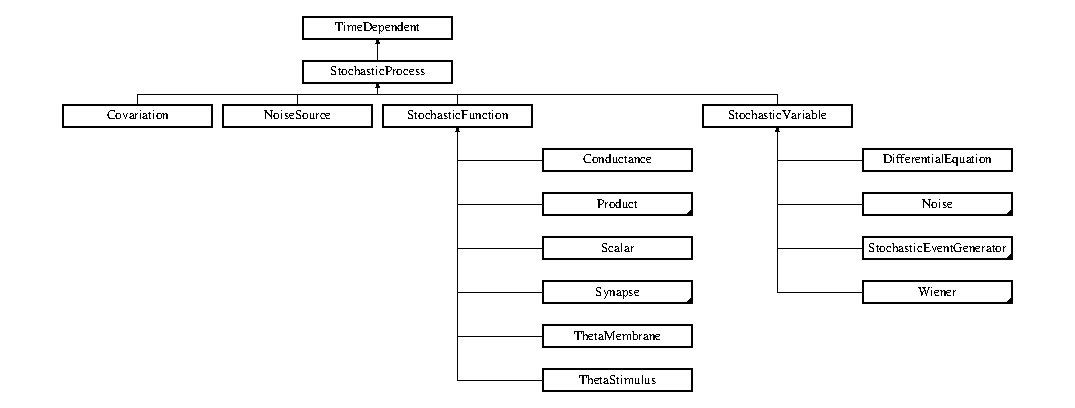
\includegraphics[height=5.02994cm]{classTimeDependent}
\end{center}
\end{figure}


\subsection{Detailed Description}
\doxyref{Time}{p.}{classTime} dependent objects. 

All objects which depend on time, especially on the size of the simulation time, must derive from this class. \subsection*{Public Member Functions}
\begin{CompactItemize}
\item 
{\bf TimeDependent} (class {\bf Time} $\ast$time)
\begin{CompactList}\small\item\em Construct. \item\end{CompactList}\item 
virtual void {\bf proceedToNextState} ()=0
\begin{CompactList}\small\item\em Proceed one time step. \item\end{CompactList}\item 
virtual void {\bf prepareNextState} ()=0
\begin{CompactList}\small\item\em Calculate next value (preparing next step). \item\end{CompactList}\item 
virtual void {\bf init} ()=0\label{classTimeDependent_363fbc0e193f877599c97972aa626c4b}

\begin{CompactList}\small\item\em Reset all time dependent values. \item\end{CompactList}\item 
virtual bool {\bf isNextStatePrepared} ()=0\label{classTimeDependent_7897befd8df8f639732bcb878559a12e}

\begin{CompactList}\small\item\em Whether the next state is prepared or not. \item\end{CompactList}\item 
virtual class {\bf Time} $\ast$ {\bf getTime} () const \label{classTimeDependent_76b3f9261a0fc8a4403d895d6bd69f3b}

\begin{CompactList}\small\item\em Return pointer to the time object. \item\end{CompactList}\end{CompactItemize}


\subsection{Constructor \& Destructor Documentation}
\index{TimeDependent@{TimeDependent}!TimeDependent@{TimeDependent}}
\index{TimeDependent@{TimeDependent}!TimeDependent@{TimeDependent}}
\subsubsection[TimeDependent]{\setlength{\rightskip}{0pt plus 5cm}TimeDependent::TimeDependent (class {\bf Time} $\ast$ {\em time})}\label{classTimeDependent_440d92de65d0a0bfd83f9a01005f5378}


Construct. 

\begin{Desc}
\item[Parameters:]
\begin{description}
\item[{\em time}]\doxyref{Time}{p.}{classTime} object on which this object is dependent If 0 is given here, a new time object with time step dt=1.0 will be created. In this case the object will be independent of all changes made to the time settings otherwise in the program. This must only be used for objects, which are not dependent on the current time settings, but inherit from this class anyway (some special forms of \doxyref{StochasticProcess}{p.}{classStochasticProcess} variables, like \doxyref{Product}{p.}{classProduct}). \end{description}
\end{Desc}


\subsection{Member Function Documentation}
\index{TimeDependent@{TimeDependent}!proceedToNextState@{proceedToNextState}}
\index{proceedToNextState@{proceedToNextState}!TimeDependent@{TimeDependent}}
\subsubsection[proceedToNextState]{\setlength{\rightskip}{0pt plus 5cm}virtual void TimeDependent::proceedToNextState ()\hspace{0.3cm}{\tt  [pure virtual]}}\label{classTimeDependent_a9908ee1a73c1e24028c8ad95cca23ad}


Proceed one time step. 

This method can be overridden to implement the proceeding of one time step. This makes new information available at the current time. (See also \doxyref{proceedToNextState()}{p.}{classTimeDependent_a9908ee1a73c1e24028c8ad95cca23ad}). The default just writes stochNextValue into stochCurrentValue. 

Implemented in {\bf IfNeuron} \doxyref{}{p.}{classIfNeuron_7604467649fbffaf8e6bf908b5cff631}, {\bf Noise} \doxyref{}{p.}{classNoise_d415a595bd0d58033aca22fee1abaa37}, {\bf NoiseSource} \doxyref{}{p.}{classNoiseSource_fd3c912f95fdbeb9e0d4fafcc0f3e320}, {\bf StochasticProcess} \doxyref{}{p.}{classStochasticProcess_c79b6846db19a8de5025a2e36b6f6901}, and {\bf SimpleSynapse} \doxyref{}{p.}{classSimpleSynapse_af49bacea075b5b2d4824a348ee2ecb2}.\index{TimeDependent@{TimeDependent}!prepareNextState@{prepareNextState}}
\index{prepareNextState@{prepareNextState}!TimeDependent@{TimeDependent}}
\subsubsection[prepareNextState]{\setlength{\rightskip}{0pt plus 5cm}virtual void TimeDependent::prepareNextState ()\hspace{0.3cm}{\tt  [pure virtual]}}\label{classTimeDependent_a6ab965445cc9bbfc7b1fe97e5610f3a}


Calculate next value (preparing next step). 

This method should be overridden to implement the calculation of the next value, using information wich is available at the current time. 

Implemented in {\bf Covariation} \doxyref{}{p.}{classCovariation_44472092d0752fb1c485012b46f4d47e}, {\bf DifferentialEquation} \doxyref{}{p.}{classDifferentialEquation_439f935ee6aac295651739607795b3f2}, {\bf IfNeuron} \doxyref{}{p.}{classIfNeuron_e511a2a61130bacf26be86fcc2dd7a91}, {\bf Noise} \doxyref{}{p.}{classNoise_8fa133802af28a8e0c84dd7eea1c22ff}, {\bf NoiseSource} \doxyref{}{p.}{classNoiseSource_a175b33b2a8f00e07ce5fa83d03e53f8}, {\bf Poisson} \doxyref{}{p.}{classPoisson_080ccca540e025812d091fdae3b4075c}, {\bf StochasticProcess} \doxyref{}{p.}{classStochasticProcess_b4c11ea89fa2d41a9f61df1ebdf04f78}, {\bf SimpleSynapse} \doxyref{}{p.}{classSimpleSynapse_4a737cab949dbf6c74e4990f7d7daeca}, {\bf ThetaNeuron} \doxyref{}{p.}{classThetaNeuron_2421556c8772c60e04701665aefa4fab}, and {\bf Wiener} \doxyref{}{p.}{classWiener_8784d5493dabf67deb75d1494450ea9b}.
\section{Unit Class Reference}
\label{classUnit}\index{Unit@{Unit}}


\subsection{Detailed Description}
A physical unit. 

This is mainly a helper class for the class \doxyref{Physical}{p.}{classPhysical}. It describes physical units such as Volt or Meter. \subsection*{Public Member Functions}
\begin{CompactItemize}
\item 
{\bf Unit} (int exp, int m, int kg, int s, int A, int K, int mol, int cd)
\begin{CompactList}\small\item\em Construct a physical unit. \item\end{CompactList}\item 
{\bf Unit} (string prefix, string name)
\begin{CompactList}\small\item\em Construct a physical unit. \item\end{CompactList}\item 
void {\bf set} (int exp, int m, int kg, int s, int A, int K, int mol, int cd)
\begin{CompactList}\small\item\em Set values. \item\end{CompactList}\item 
void {\bf set} (int m, int kg, int s, int A, int K, int mol, int cd)
\begin{CompactList}\small\item\em Set values. \item\end{CompactList}\item 
{\bf Unit} ()\label{classUnit_8e46f663a95736c8002d85ab271a7581}

\begin{CompactList}\small\item\em Simple constructor. \item\end{CompactList}\item 
{\bf Unit} (const {\bf Unit} \&)\label{classUnit_e7351c99c228ee3bad29e47a8716aa22}

\begin{CompactList}\small\item\em Copy constructor. \item\end{CompactList}\item 
string {\bf getSymbol} ()
\begin{CompactList}\small\item\em Get name. \item\end{CompactList}\item 
string {\bf getName} ()
\begin{CompactList}\small\item\em Get long name. \item\end{CompactList}\item 
void {\bf setPrefix} (int n)
\begin{CompactList}\small\item\em Set the prefix. \item\end{CompactList}\end{CompactItemize}


\subsection{Constructor \& Destructor Documentation}
\index{Unit@{Unit}!Unit@{Unit}}
\index{Unit@{Unit}!Unit@{Unit}}
\subsubsection[Unit]{\setlength{\rightskip}{0pt plus 5cm}Unit::Unit (int {\em exp}, \/  int {\em m}, \/  int {\em kg}, \/  int {\em s}, \/  int {\em A}, \/  int {\em K}, \/  int {\em mol}, \/  int {\em cd})}\label{classUnit_22c52a75de2e92c258e3e4e24dffc20d}


Construct a physical unit. 

\begin{Desc}
\item[Parameters:]
\begin{description}
\item[{\em exp}]Prefix \item[{\em m}]Meters \item[{\em kg}]Kilograms \item[{\em s}]Seconds \item[{\em A}]Ampere \item[{\em K}]Kelvin \item[{\em mol}]Mole \item[{\em cd}]Candela Construct a unit. The prefix's exponent (like -3 for milli, 0 for nothing or 3 for kilo), and the exponents of the individual SI units have to be given. Example: if acceleration is given as -3 km/s$^\wedge$2, the constructor must be called as \doxyref{Unit}{p.}{classUnit}(3, 1,0,-2,0,0,0). \end{description}
\end{Desc}
\index{Unit@{Unit}!Unit@{Unit}}
\index{Unit@{Unit}!Unit@{Unit}}
\subsubsection[Unit]{\setlength{\rightskip}{0pt plus 5cm}Unit::Unit (string {\em prefix}, \/  string {\em name})}\label{classUnit_64ea05a89e6077d8ffb6978cdee8205c}


Construct a physical unit. 

\doxyref{Unit}{p.}{classUnit} u('m','V'); 

\subsection{Member Function Documentation}
\index{Unit@{Unit}!set@{set}}
\index{set@{set}!Unit@{Unit}}
\subsubsection[set]{\setlength{\rightskip}{0pt plus 5cm}void Unit::set (int {\em exp}, \/  int {\em m}, \/  int {\em kg}, \/  int {\em s}, \/  int {\em A}, \/  int {\em K}, \/  int {\em mol}, \/  int {\em cd})}\label{classUnit_476cbf01f18493f915833379784452f9}


Set values. 

\begin{Desc}
\item[Parameters:]
\begin{description}
\item[{\em exp}]Prefix \item[{\em m}]Meters \item[{\em kg}]Kilograms \item[{\em s}]Seconds \item[{\em A}]Ampere \item[{\em K}]Kelvin \item[{\em mol}]Mole \item[{\em cd}]Candela Construct a unit. The prefix's exponent (like -3 for milli, 0 for nothing or 3 for kilo), and the exponents of the individual SI units have to be given. Example: if acceleration is given as -3 km/s$^\wedge$2, the constructor must be called as \doxyref{Unit}{p.}{classUnit}(3, 1,0,-2,0,0,0). \end{description}
\end{Desc}
\index{Unit@{Unit}!set@{set}}
\index{set@{set}!Unit@{Unit}}
\subsubsection[set]{\setlength{\rightskip}{0pt plus 5cm}void Unit::set (int {\em m}, \/  int {\em kg}, \/  int {\em s}, \/  int {\em A}, \/  int {\em K}, \/  int {\em mol}, \/  int {\em cd})}\label{classUnit_f1141b3d28d5686484eff81e521dfea7}


Set values. 

\begin{Desc}
\item[Parameters:]
\begin{description}
\item[{\em m}]Meters \item[{\em kg}]Kilograms \item[{\em s}]Seconds \item[{\em A}]Ampere \item[{\em K}]Kelvin \item[{\em mol}]Mole \item[{\em cd}]Candela Construct a unit. The prefix's exponent (like -3 for milli, 0 for nothing or 3 for kilo), and the exponents of the individual SI units have to be given. Example: if acceleration is given as -3 km/s$^\wedge$2, the constructor must be called as \doxyref{Unit}{p.}{classUnit}(3, 1,0,-2,0,0,0). \end{description}
\end{Desc}
\index{Unit@{Unit}!getSymbol@{getSymbol}}
\index{getSymbol@{getSymbol}!Unit@{Unit}}
\subsubsection[getSymbol]{\setlength{\rightskip}{0pt plus 5cm}string Unit::getSymbol ()}\label{classUnit_884a258351ba026ae471462574734826}


Get name. 

This retrieves the name as symbol, f.e. 'mV'. Note that you have to set the description for yourself. \index{Unit@{Unit}!getName@{getName}}
\index{getName@{getName}!Unit@{Unit}}
\subsubsection[getName]{\setlength{\rightskip}{0pt plus 5cm}string Unit::getName ()}\label{classUnit_fafe0245ccc9acafc4c9107d0def12b9}


Get long name. 

This retrieves the complete name, like 'millivolt'. Note that the long name is not always existant. (A unit like s$^\wedge$4 will have no long name.) \index{Unit@{Unit}!setPrefix@{setPrefix}}
\index{setPrefix@{setPrefix}!Unit@{Unit}}
\subsubsection[setPrefix]{\setlength{\rightskip}{0pt plus 5cm}void Unit::setPrefix (int {\em n})}\label{classUnit_7b55eb99fa7d0aa48821694ea8168a87}


Set the prefix. 

Set the prefix by giving an integer from -24 to 24. Should be a multiple of 3, exception: -2,-1,2,1. 
\section{Wiener Class Reference}
\label{classWiener}\index{Wiener@{Wiener}}
Inheritance diagram for Wiener::\begin{figure}[H]
\begin{center}
\leavevmode
\includegraphics[height=5cm]{classWiener}
\end{center}
\end{figure}


\subsection{Detailed Description}
Properties for all \doxyref{Wiener}{p.}{classWiener} processes. 

Standard Functions of \doxyref{Wiener}{p.}{classWiener} processes. This class implements a \doxyref{Wiener}{p.}{classWiener} processes. The process can have a time-proportional mean $\mu t$ and variance $\sigma^2 t$. \subsection*{Public Member Functions}
\begin{CompactItemize}
\item 
virtual void {\bf init} ()\label{classWiener_605e29d819949fa5c4220aa09dd212ea}

\begin{CompactList}\small\item\em Initialise time-dependent values. \item\end{CompactList}\item 
virtual void {\bf prepareNextState} ()
\begin{CompactList}\small\item\em Calculate next value (preparing next step). \item\end{CompactList}\item 
virtual string {\bf getParameter} (const string \&)
\begin{CompactList}\small\item\em Get parameter. \item\end{CompactList}\item 
virtual void {\bf setParameter} (const string \&, const string \&)
\begin{CompactList}\small\item\em Set parameter. \item\end{CompactList}\end{CompactItemize}


\subsection{Member Function Documentation}
\index{Wiener@{Wiener}!prepareNextState@{prepareNextState}}
\index{prepareNextState@{prepareNextState}!Wiener@{Wiener}}
\subsubsection[prepareNextState]{\setlength{\rightskip}{0pt plus 5cm}virtual void Wiener::prepareNextState ()\hspace{0.3cm}{\tt  [virtual]}}\label{classWiener_8784d5493dabf67deb75d1494450ea9b}


Calculate next value (preparing next step). 

This method should be overridden to implement the calculation of the next value, using information wich is available at the current time. The method sets stochNextStateIsPrepared to true if successful. 

Reimplemented from {\bf StochasticProcess} \doxyref{}{p.}{classStochasticProcess_b4c11ea89fa2d41a9f61df1ebdf04f78}.\index{Wiener@{Wiener}!getParameter@{getParameter}}
\index{getParameter@{getParameter}!Wiener@{Wiener}}
\subsubsection[getParameter]{\setlength{\rightskip}{0pt plus 5cm}virtual string Wiener::getParameter (const string \& {\em name})\hspace{0.3cm}{\tt  [virtual]}}\label{classWiener_313637cdbd6ae2865897bf48fa1ced4b}


Get parameter. 

In a derived class, override this to handle every parameter you implement. If a parameter is described using multiple strings separated by space, this indicates a parameter of a parameter. 

Reimplemented from {\bf Parametric} \doxyref{}{p.}{classParametric_3c39188e1750b8e5d442b9dfa079b1c8}.

Reimplemented in {\bf WienerCpp} \doxyref{}{p.}{classWienerCpp_6e9dd9a019c621a7990f4133d476c92c}.\index{Wiener@{Wiener}!setParameter@{setParameter}}
\index{setParameter@{setParameter}!Wiener@{Wiener}}
\subsubsection[setParameter]{\setlength{\rightskip}{0pt plus 5cm}virtual void Wiener::setParameter (const string \& {\em name}, \/  const string \& {\em value})\hspace{0.3cm}{\tt  [virtual]}}\label{classWiener_69c25adbb4bcad391350812d7f59f84c}


Set parameter. 

Sets the value of a parameter using strings. If a parameter is described using multiple strings separated by space, this indicates a parameter of a parameter (not implemented yet). 

Reimplemented from {\bf Parametric} \doxyref{}{p.}{classParametric_bba36dc4545219658541ab55251e02e6}.

Reimplemented in {\bf WienerCpp} \doxyref{}{p.}{classWienerCpp_afdaaadb8175a259d4bc420c823829a0}.
\section{WienerCpp Class Reference}
\label{classWienerCpp}\index{WienerCpp@{WienerCpp}}
Inheritance diagram for WienerCpp::\begin{figure}[H]
\begin{center}
\leavevmode
\includegraphics[height=5cm]{classWienerCpp}
\end{center}
\end{figure}


\subsection{Detailed Description}
Condensed \doxyref{Poisson}{p.}{classPoisson} Process. 

Lets assume a set of \doxyref{Poisson}{p.}{classPoisson} process $s^i_t, i=1..n$, where $t$ denotes time, and $i$ is the index of the process. Each process is multiplied by a weight $w_i$, $s^i_t$ takes values of $0$ or $1$ (where $1$ indicates an event), and events occur with a rate of $\lambda_i$. We are interested in the sum \[s_t = \sum_i w_i s^i_t.\] Let's assume that in this collection of events coincident events happen. Coincidences are events which occur at the same time at various processes. If these events are viewed as a separate process $s^c_i$ with a weight $w_c$ and a rate $\lambda_c$, all processes stay independent. The impact of the coincidence events depends on the sum of the weights of the processes taking part. We shall call the sum of the weights of the processes which take part the {\em Coincidence Weight\/}. The coincidences occur with a specific rate which we will call {\em Coincidence Rate\/} $\lambda_c$.

Since the events which form the coincidence event are taken out of the process $s_i$ where the happened, the rate of these single processes is expected to decrease, according to the coincidence weight and the coincidence rate: $\lambda_i$ will become $\lambda_i - \frac{w_c\lambda_c}{\sum_iw_i}$. Thus the sum of events $s_t$, as well as its mean $\mbox{E}{s_t}$ will not be affected by the correlations: \[ s_t = \sum_{i}w_is^i_t + w_cs^c_t. \] \[ \mbox{E}{s_t} = \sum_i w_i\left(\lambda_i - \frac{w_c\lambda_c}{\sum_iw_i}\right) + w_c\lambda_c \] \[ = \sum_i w_i\lambda_i \] The variance of this process $s_t$ will be: \[\mbox{Var}\{s_t\} = \sum_i w_i^2\left(\lambda_i - \frac{w_c\lambda_c}{\sum_iw_i}\right) + w_c^2\lambda_c.\]

These parameters will be used to construct a white-noise (\doxyref{Wiener}{p.}{classWiener}) process, which feeds the neuron: Let's assume the neuron is connected to many synapses which each have small weights. Lets substitute the correlation weight $w_c$ - since all weights are the same - by the amount $n_c$ of synapses taking part in a coincident pulse times their weight. We will call this amount the {\em Coincidence Width\/}.

Since the \{coincidence rate\} $\lambda_c$ will not be higher than the overall rate $\lambda$, and the \{coincidence width\} $n_c$ will not be higher than the overall number of synapses, it makes sense to use a {\em relative coincidence width\/} which ranges from $0$ to $1$ \[n_{rc} = \frac{n_c}{n},\] and a {\em relative coincidence rate\/} which ranges from $0$ to $1$ \[\lambda_{rc} = \frac{\lambda_c}{\lambda}\] This amounts to the following expressions for mean and variance of the white-noise process:

\[ \mu := nw\lambda \] \[ \sigma^2 := nw^2\lambda\left(1 - n_{rc} \lambda_{rc} + nn_{rc}^2\lambda_{rc} \right) \]

The condensed poisson process implements such a white-noise process. \subsection*{Public Member Functions}
\begin{CompactItemize}
\item 
{\bf WienerCpp} (class {\bf Time} $\ast$time, double w, double n, double lambda, double n\_\-rc, double lambda\_\-rc)
\begin{CompactList}\small\item\em Constructor. \item\end{CompactList}\item 
virtual string {\bf getParameter} (const string \&p)
\begin{CompactList}\small\item\em Get parameter. \item\end{CompactList}\item 
virtual void {\bf setParameter} (const string \&p, const string \&d)
\begin{CompactList}\small\item\em Set parameter. \item\end{CompactList}\item 
virtual void {\bf init} ()\label{classWienerCpp_d7abd3762ed4a99455e6edcadb7d24cc}

\begin{CompactList}\small\item\em Initialise time-dependent values. \item\end{CompactList}\end{CompactItemize}


\subsection{Constructor \& Destructor Documentation}
\index{WienerCpp@{WienerCpp}!WienerCpp@{WienerCpp}}
\index{WienerCpp@{WienerCpp}!WienerCpp@{WienerCpp}}
\subsubsection[WienerCpp]{\setlength{\rightskip}{0pt plus 5cm}WienerCpp::WienerCpp (class {\bf Time} $\ast$ {\em time}, \/  double {\em w}, \/  double {\em n}, \/  double {\em lambda}, \/  double {\em n\_\-rc}, \/  double {\em lambda\_\-rc})}\label{classWienerCpp_2f68b6afbd1edfe84650287cbd9d2d12}


Constructor. 

\begin{Desc}
\item[Parameters:]
\begin{description}
\item[{\em time}]\doxyref{Time}{p.}{classTime} object \item[{\em w}]single weight \item[{\em n}]number of processes in the sum of processes \item[{\em lambda}]rate of a single process \item[{\em n\_\-rc}]relative coincidence width \item[{\em lambda\_\-rc}]relative coincidence height \end{description}
\end{Desc}


\subsection{Member Function Documentation}
\index{WienerCpp@{WienerCpp}!getParameter@{getParameter}}
\index{getParameter@{getParameter}!WienerCpp@{WienerCpp}}
\subsubsection[getParameter]{\setlength{\rightskip}{0pt plus 5cm}virtual string WienerCpp::getParameter (const string \& {\em name})\hspace{0.3cm}{\tt  [virtual]}}\label{classWienerCpp_6e9dd9a019c621a7990f4133d476c92c}


Get parameter. 

In a derived class, override this to handle every parameter you implement. If a parameter is described using multiple strings separated by space, this indicates a parameter of a parameter. 

Reimplemented from {\bf Wiener} \doxyref{}{p.}{classWiener_313637cdbd6ae2865897bf48fa1ced4b}.\index{WienerCpp@{WienerCpp}!setParameter@{setParameter}}
\index{setParameter@{setParameter}!WienerCpp@{WienerCpp}}
\subsubsection[setParameter]{\setlength{\rightskip}{0pt plus 5cm}virtual void WienerCpp::setParameter (const string \& {\em name}, \/  const string \& {\em value})\hspace{0.3cm}{\tt  [virtual]}}\label{classWienerCpp_afdaaadb8175a259d4bc420c823829a0}


Set parameter. 

Sets the value of a parameter using strings. If a parameter is described using multiple strings separated by space, this indicates a parameter of a parameter (not implemented yet). 

Reimplemented from {\bf Wiener} \doxyref{}{p.}{classWiener_69c25adbb4bcad391350812d7f59f84c}.
\section{WienerNoise Class Reference}
\label{classWienerNoise}\index{WienerNoise@{WienerNoise}}
Inheritance diagram for WienerNoise::\begin{figure}[H]
\begin{center}
\leavevmode
\includegraphics[height=5cm]{classWienerNoise}
\end{center}
\end{figure}


\subsection{Detailed Description}
A \doxyref{Wiener}{p.}{classWiener} process (white) noise source. 

Internal class: You never need to acces this class directly, since all public members are defined in \doxyref{Noise}{p.}{classNoise}. This special derivation of \doxyref{Noise}{p.}{classNoise} is only important internally, for the \doxyref{NoiseSource}{p.}{classNoiseSource} class. \subsection*{Protected Member Functions}
\begin{CompactItemize}
\item 
{\bf WienerNoise} (class {\bf NoiseSource} $\ast$parent, int index, const string \&name=\char`\"{}\char`\"{}, const string \&type=\char`\"{}correlated\_\-wiener\_\-process\char`\"{})
\begin{CompactList}\small\item\em Construct. \item\end{CompactList}\item 
{\bf WienerNoise} (const {\bf WienerNoise} \&)
\begin{CompactList}\small\item\em Construct. \item\end{CompactList}\item 
virtual void {\bf setNext} (double indicator)
\begin{CompactList}\small\item\em Set the next values. \item\end{CompactList}\end{CompactItemize}
\subsection*{Friends}
\begin{CompactItemize}
\item 
class {\bf NoiseSource}\label{classWienerNoise_14268df5638debed66cad6d85946916f}

\end{CompactItemize}


\subsection{Constructor \& Destructor Documentation}
\index{WienerNoise@{WienerNoise}!WienerNoise@{WienerNoise}}
\index{WienerNoise@{WienerNoise}!WienerNoise@{WienerNoise}}
\subsubsection[WienerNoise]{\setlength{\rightskip}{0pt plus 5cm}WienerNoise::WienerNoise (class {\bf NoiseSource} $\ast$ {\em parent}, \/  int {\em index}, \/  const string \& {\em name} = {\tt \char`\"{}\char`\"{}}, \/  const string \& {\em type} = {\tt \char`\"{}correlated\_\-wiener\_\-process\char`\"{}})\hspace{0.3cm}{\tt  [protected]}}\label{classWienerNoise_11d57548e324527ca0e82391bd6640d2}


Construct. 

This constructor is protected, because this class can only be instantiated by calls from the \doxyref{NoiseSource}{p.}{classNoiseSource} class. \index{WienerNoise@{WienerNoise}!WienerNoise@{WienerNoise}}
\index{WienerNoise@{WienerNoise}!WienerNoise@{WienerNoise}}
\subsubsection[WienerNoise]{\setlength{\rightskip}{0pt plus 5cm}WienerNoise::WienerNoise (const {\bf WienerNoise} \&)\hspace{0.3cm}{\tt  [protected]}}\label{classWienerNoise_312b3a41b91f25610bac9f198701716d}


Construct. 

This class mustn't be copied. 

\subsection{Member Function Documentation}
\index{WienerNoise@{WienerNoise}!setNext@{setNext}}
\index{setNext@{setNext}!WienerNoise@{WienerNoise}}
\subsubsection[setNext]{\setlength{\rightskip}{0pt plus 5cm}virtual void WienerNoise::setNext (double {\em indicator})\hspace{0.3cm}{\tt  [protected, virtual]}}\label{classWienerNoise_562ca2825d5fc8bed63339893b6abbbb}


Set the next values. 

\begin{Desc}
\item[Parameters:]
\begin{description}
\item[{\em indicator}]The stochastic indicator. This is the main method. The \doxyref{NoiseSource}{p.}{classNoiseSource} class uses this to set the indicator values. If the indicator is above the current threshold, the value is set to w (the weight of the process), otherwise to 0.0. \end{description}
\end{Desc}


Implements {\bf Noise} \doxyref{}{p.}{classNoise}.
\printindex
\end{document}
